% Options for packages loaded elsewhere
\PassOptionsToPackage{unicode}{hyperref}
\PassOptionsToPackage{hyphens}{url}
\PassOptionsToPackage{dvipsnames,svgnames,x11names}{xcolor}
\documentclass[
  spanish,
  a4paper,
  openany]{book}
\usepackage{xcolor}
\usepackage[top=1in,bottom=1in,right=1in,left=1in]{geometry}
\usepackage{amsmath,amssymb}
\setcounter{secnumdepth}{5}
\usepackage{iftex}
\ifPDFTeX
  \usepackage[T1]{fontenc}
  \usepackage[utf8]{inputenc}
  \usepackage{textcomp} % provide euro and other symbols
\else % if luatex or xetex
  \usepackage{unicode-math} % this also loads fontspec
  \defaultfontfeatures{Scale=MatchLowercase}
  \defaultfontfeatures[\rmfamily]{Ligatures=TeX,Scale=1}
\fi
\usepackage[]{bookman}
\ifPDFTeX\else
  % xetex/luatex font selection
\fi
% Use upquote if available, for straight quotes in verbatim environments
\IfFileExists{upquote.sty}{\usepackage{upquote}}{}
\IfFileExists{microtype.sty}{% use microtype if available
  \usepackage[]{microtype}
  \UseMicrotypeSet[protrusion]{basicmath} % disable protrusion for tt fonts
}{}
\makeatletter
\@ifundefined{KOMAClassName}{% if non-KOMA class
  \IfFileExists{parskip.sty}{%
    \usepackage{parskip}
  }{% else
    \setlength{\parindent}{0pt}
    \setlength{\parskip}{6pt plus 2pt minus 1pt}}
}{% if KOMA class
  \KOMAoptions{parskip=half}}
\makeatother
\usepackage{longtable,booktabs,array}
\newcounter{none} % for unnumbered tables
\usepackage{calc} % for calculating minipage widths
% Correct order of tables after \paragraph or \subparagraph
\usepackage{etoolbox}
\makeatletter
\patchcmd\longtable{\par}{\if@noskipsec\mbox{}\fi\par}{}{}
\makeatother
% Allow footnotes in longtable head/foot
\IfFileExists{footnotehyper.sty}{\usepackage{footnotehyper}}{\usepackage{footnote}}
\makesavenoteenv{longtable}
\usepackage{graphicx}
\makeatletter
\newsavebox\pandoc@box
\newcommand*\pandocbounded[1]{% scales image to fit in text height/width
  \sbox\pandoc@box{#1}%
  \Gscale@div\@tempa{\textheight}{\dimexpr\ht\pandoc@box+\dp\pandoc@box\relax}%
  \Gscale@div\@tempb{\linewidth}{\wd\pandoc@box}%
  \ifdim\@tempb\p@<\@tempa\p@\let\@tempa\@tempb\fi% select the smaller of both
  \ifdim\@tempa\p@<\p@\scalebox{\@tempa}{\usebox\pandoc@box}%
  \else\usebox{\pandoc@box}%
  \fi%
}
% Set default figure placement to htbp
\def\fps@figure{htbp}
\makeatother
\ifLuaTeX
\usepackage[bidi=basic,shorthands=off]{babel}
\else
\usepackage[bidi=default,shorthands=off]{babel}
\fi
\ifLuaTeX
  \usepackage{selnolig} % disable illegal ligatures
\fi
\setlength{\emergencystretch}{3em} % prevent overfull lines
\providecommand{\tightlist}{%
  \setlength{\itemsep}{0pt}\setlength{\parskip}{0pt}}
\usepackage[]{natbib}
\bibliographystyle{apalike}
\usepackage{graphicx}
\usepackage{fancyhdr}
\pagestyle{plain}
\renewcommand{\headrulewidth}{0.2pt}
\usepackage{floatpag}
\floatpagestyle{empty}
\usepackage{bookmark}
\IfFileExists{xurl.sty}{\usepackage{xurl}}{} % add URL line breaks if available
\urlstyle{same}
\hypersetup{
  pdftitle={Ciberseguridad ciudadana},
  pdfauthor={Diego Chiquero Mena},
  pdflang={es},
  pdfkeywords={seguridad, privacidad, ciberdelitos, ciberdelincuentes, ciberseguridad ciudadana, internet, inteligencia artificial},
  colorlinks=true,
  linkcolor={blue},
  filecolor={Maroon},
  citecolor={Blue},
  urlcolor={Blue},
  pdfcreator={LaTeX via pandoc}}

\title{Ciberseguridad ciudadana}
\author{Diego Chiquero Mena}
\date{06 September 2026}

\begin{document}
\maketitle

\thispagestyle{empty}
\begin{center}
\noindent\makebox[\textwidth]{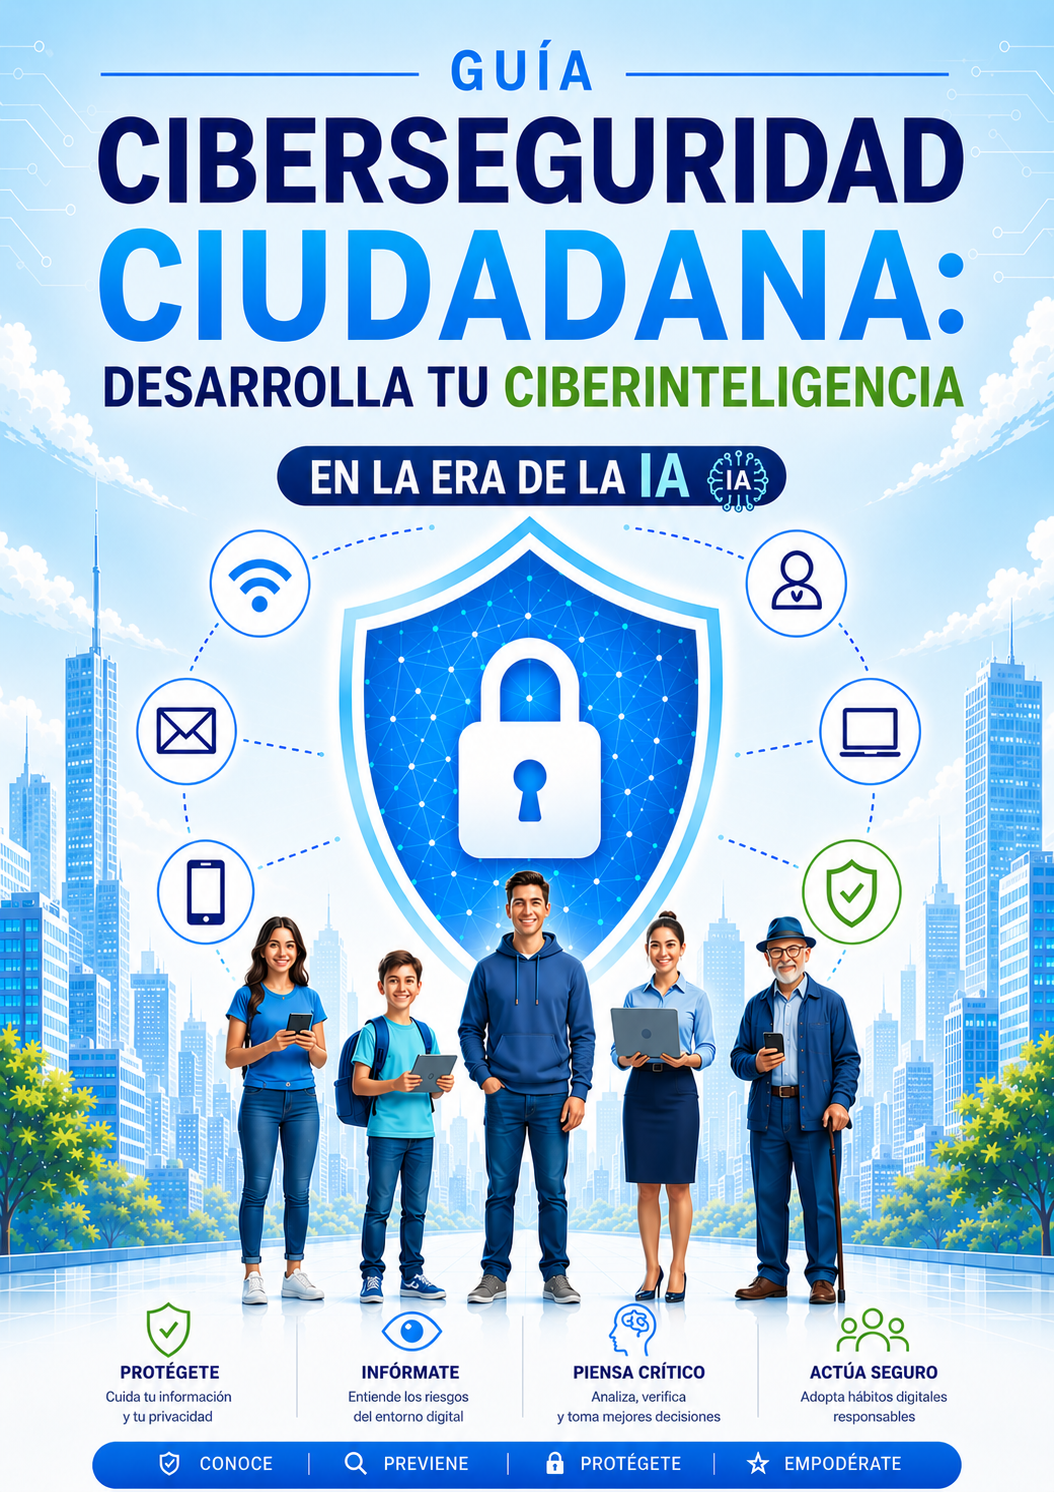
\includegraphics[width=\paperwidth]{images/cover.png}}
%\makebox[\textwidth]{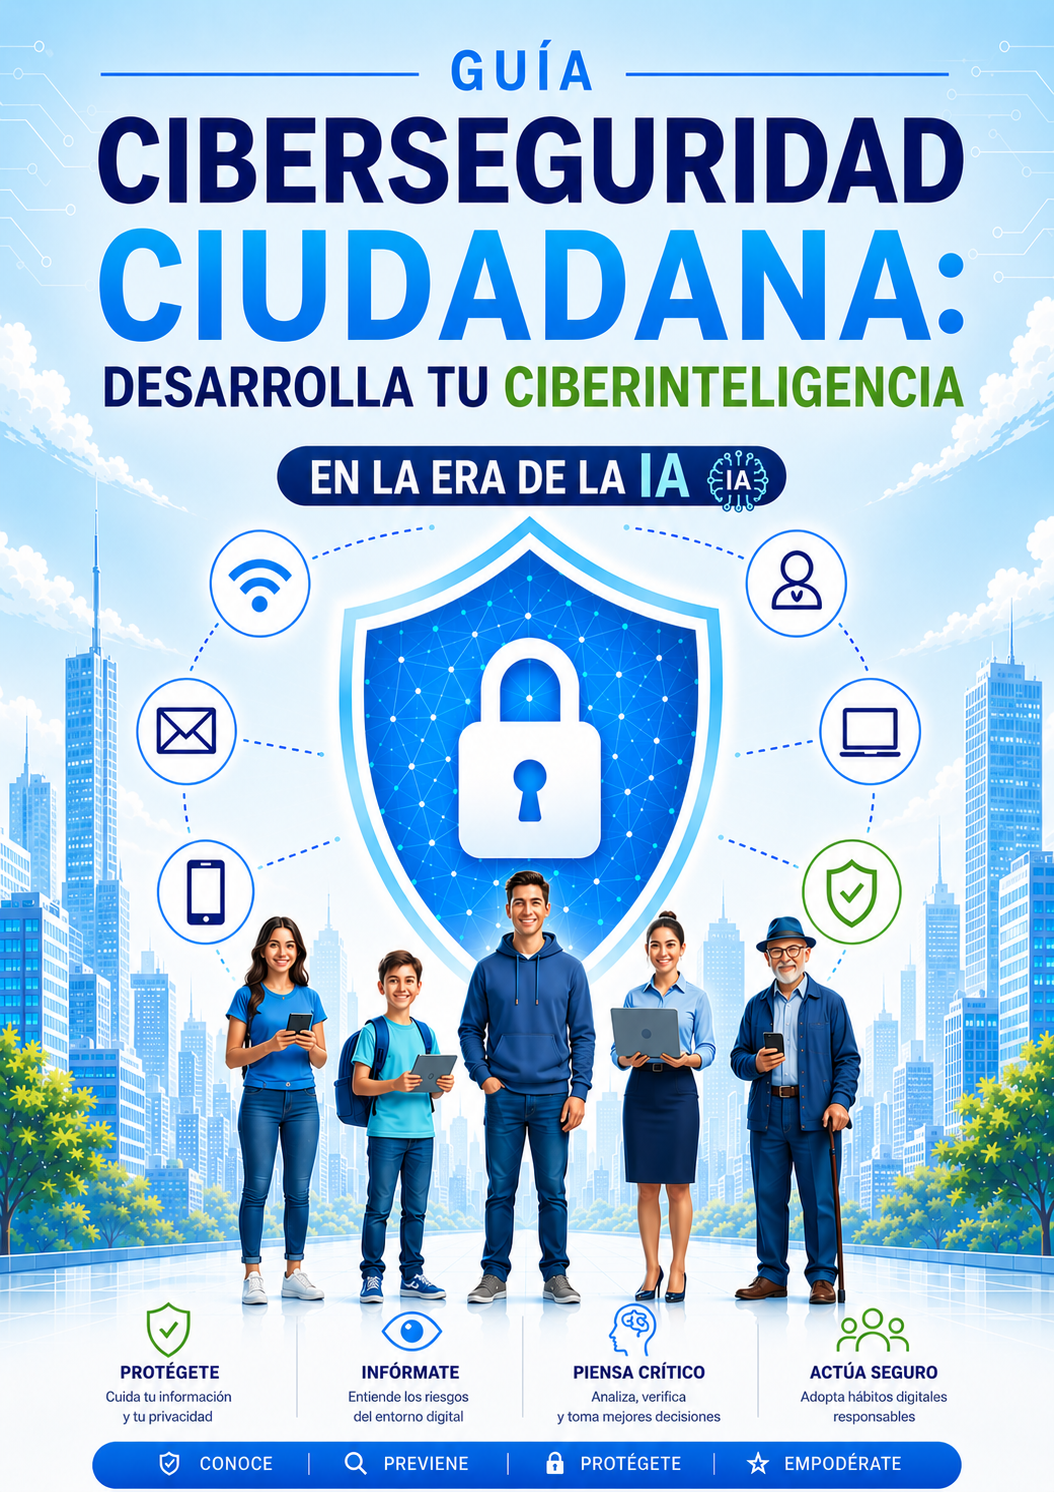
\includegraphics[width=\paperwidth]{images/cover.png}}
\end{center}
\fontsize{14}{16}
%\fontseries{b}
\selectfont





{
\setcounter{tocdepth}{3}
\tableofcontents
}
\chapter*{Prólogo}\label{pruxf3logo}
\addcontentsline{toc}{chapter}{Prólogo}

Esta guía aglutina de manera filtrada y tamizada una amplia y detallada parte del conocimiento e información de relevancia que puedes encontrar en la web sobre privacidad y seguridad en internet, de forma ordenada y estructurada. Además, encontrarás en la bibliografía todas las fuentes que han hecho posible la elaboración y documentación de esta guía, para que puedas contrastar por ti mismo dichas fuentes.

Entenderás las diferencias entre los conceptos de privacidad y seguridad en internet, para que de este modo puedas hacer una buena configuración y uso de éstas.

Aprenderás buenas prácticas en la gestión de la privacidad, así como la manera más adecuada de gestionar la seguridad tanto en los equipos (PC, tables, smartphones, etc.), como en la red de datos.

Conocerás las principales amenazas que existen en el uso de las tecnologías y el mundo digital.

Por último, pero no por ello menos importante, se abordarán otros conceptos relacionados con los ciberdelitos, la huella digital, la importancia de ser selectivos con la información online y otros aspectos más.

Todo ello actualizado al contexto actual, donde la inteligencia artificial forma parte de nuestro día a día digital: entenderás cómo estas tecnologías amplifican tanto las oportunidades como los riesgos, cómo afectan a tu privacidad, cómo pueden utilizarse para manipular, perfilar o automatizar ataques, y qué medidas prácticas puedes tomar para protegerte en un entorno donde la frontera entre lo humano y lo automatizado es cada vez más difusa.

También encontrarás a lo largo de la guía, multitud de enlaces que te llevarán a más información ampliada sobre las temáticas, así como una extensa lista de recursos y herramientas para que puedas llevar tu privacidad y seguridad en internet al siguiente nivel.

Si quieres contribuir y ayudar a nutrir de más contenido de valor esta guía, por favor, no lo dudes y ponte en contacto conmigo, estaré encantado que colaboremos. Encontrarás mis datos de contacto en el siguiente apartado \emph{sobre el autor}.

Esta guía está disponible en el repositorio Github: \href{https://github.com/diegochiquero/ciberseguridad-ciudadana}{diegochiquero/ciberseguridad-ciudadana}. Y ha sido escrito en \href{http://rmarkdown.rstudio.com}{R-Markdown} empleando el paquete \href{https://bookdown.org/}{\texttt{bookdown}} cuya guia encontrarás en \citep{R-bookdown}.

Esta obra está bajo la \href{https://creativecommons.org/licenses/by-nc-sa/4.0/deed.es}{licencia Creative Commons Atribución-NoComercial-CompartirIgual 4.0 Internacional}.

\begin{flushleft}\includegraphics{images/by-nc-sa-88x31} \end{flushleft}

\chapter*{Sobre el autor}\label{autor}
\addcontentsline{toc}{chapter}{Sobre el autor}

\begin{flushleft}\includegraphics[width=0.25\linewidth]{images/diego-chiquero-m-2023-profile} \end{flushleft}

Hola, mi nombre es Diego.

Y lo primero que me gustaría hacer es agradecerte que hayas decidido leer esta guía. Ese simple gesto hace que todas las horas de dedicación, esfuerzo, documentación, contraste de fuentes y curación de contenidos hayan merecido la pena. Mi propósito aquí es acompañarte: ayudarte a tomar conciencia de los peligros reales de navegar por internet, de lo expuesto que puedes llegar a estar en tu día a día digital y, al mismo tiempo, darte herramientas prácticas para gestionar la tecnología de forma segura, privada y con más control.

Soy desarrollador web full stack, emprendedor tecnológico y divulgador autodidacta especializado en lo que se conoce como ciberseguridad ciudadana: una forma de entender la privacidad y la seguridad en el ambito digital que va más allá de simplemente proteger tus dispositivos. Se trata de adquirir hábitos, criterio y autonomía para relacionarnos con la tecnología desde la consciencia y no desde el miedo.

Desde Málaga (Andalucía), donde trabajo como profesional independiente, llevo años acompañando a personas y comunidades a comprender su entorno digital sin tecnicismos innecesarios. Mi enfoque nace de la experiencia directa: aprender por curiosidad, equivocarse, documentarlo todo y convertir ese aprendizaje en guías claras y reproducibles.

Participo en talleres, charlas y proyectos comunitarios donde transformo dudas reales en prácticas sencillas que cualquiera puede aplicar. Para mí, la privacidad y la seguridad en el uso y disfrute de las TIC no es solo una batería de conceptos o soluciones rápidas, sino una actitud y una filosofía para prestar atención, entender lo que hacemos y tomar decisiones informadas en un mundo cada vez más automatizado.

En la era de la inteligencia artificial, mi objetivo es ayudarte a navegar un ecosistema donde la tecnología es poderosa, pero también opaca. Aspiro a que esta guía te sirva para usar esta nueva era tecnológica con más conciencia, más control y menos fricción.

Diego Chiquero Mena

Puedes contactar conmigo en \href{mailto:hola@diegochiquero.com}{\nolinkurl{hola@diegochiquero.com}}

Más sobre mí \href{https://diegochiquero.com}{Diego Chiquero Mena}

\chapter{Privacidad y Seguridad en Internet}\label{privacidad-y-seguridad-en-internet}

\section{Introducción}\label{introducciuxf3n}

En las últimas décadas, la evolución de las tecnologías digitales ha transformado profundamente nuestra forma de comunicarnos, informarnos, trabajar, comprar y relacionarnos. Esta transformación puede entenderse como un proceso progresivo en varias etapas.

En una primera fase, conocida como Web 1.0, internet era fundamentalmente un entorno de consulta. Las personas usuarias accedían a páginas web estáticas donde el contenido era creado por unos pocos y consumido por muchos, con una interacción muy limitada.

Posteriormente, con la llegada de la Web 2.0, internet se volvió social e interactivo. Las personas pasaron de ser simples consumidoras de información a creadoras activas de contenido. Surgieron las redes sociales, los blogs, las plataformas de vídeo y los servicios colaborativos, permitiendo publicar y compartir fácilmente fotografías, vídeos, opiniones, reseñas o mensajes desde cualquier dispositivo, como ordenadores, tabletas o teléfonos móviles.

Más recientemente, se ha extendido el concepto de Web 3.0, asociado a una web más descentralizada, personalizada y basada en tecnologías como el blockchain, los datos semánticos o las identidades digitales. Aunque su definición no es única ni está completamente consolidada, esta etapa refleja una mayor preocupación por el control de los datos, la privacidad y la autonomía de las personas usuarias.

En paralelo, estamos entrando en una nueva etapa marcada por la expansión de la inteligencia artificial. A diferencia de las anteriores, esta fase no tiene todavía una denominación universalmente aceptada (a veces se habla de Web 4.0, web inteligente o internet cognitiva), pero su impacto es evidente: los sistemas digitales ya no solo almacenan y transmiten información, sino que son capaces de generarla, interpretarla y adaptarla automáticamente.

La incorporación de la inteligencia artificial está cambiando radicalmente el entorno digital. Hoy es posible crear textos, imágenes, audios o vídeos de forma automatizada, personalizar contenidos a gran escala y simular comportamientos humanos con gran realismo. Esto amplía las oportunidades, pero también introduce nuevos riesgos, como la desinformación avanzada, la suplantación de identidad mediante deepfakes o voice hacking, los fraudes automatizados o la manipulación personalizada.

Además, los servicios digitales forman parte esencial de la vida cotidiana: banca online, compras por internet, trámites administrativos, educación, sanidad, almacenamiento en la nube o mensajería instantánea. Todo ello incrementa nuestra presencia en el entorno digital y, con ello, nuestra superficie de exposición a posibles amenazas que cada vez son más ubicuas.

Como consecuencia de ello, el enorme volumen de información sensible disponible en internet hace que las personas usuarias estemos en el punto de mira de ciberdelincuentes y expuestas a todo tipo de ciberataques. En este contexto, esta guía tiene como objetivo enseñarte, orientarte y proporcionarte herramientas prácticas para prevenir, evitar y, en la medida de lo posible, paliar los riesgos asociados al uso cotidiano de la tecnología.

Por lo tanto, a lo largo de ella, irás comprendiendo la importancia de velar de manera activa por tu privacidad y seguridad en internet, mediante una gestión adecuada de ambas. También te ayudará a conocer y reconocer los ciberdelitos más habituales en la actualidad, así como las estrategias más comunes utilizadas para llevarlos a cabo.

La ciberseguridad ciudadana se centra en protegerte, cuidando tu información y tu privacidad, en informarte para entender los riesgos del entorno digital, para que actúes con pensamiento crítico, capacidad analítica y toma de decisiones y en actuar de manera segura adoptando hábitos digitales responsables y prudentes.

\section{Privacidad}\label{privacidad}

Antes de abordar la privacidad en el ámbito digital, vamos a conceptualizarla en el mundo analógico, para ponernos en contexto; por lo tanto la privacidad es aquello que se lleva a cabo en un ámbito reservado.

Este concepto llevado al terreno digital, se entiende como el derecho y la capacidad que tienes como usuario de la red, a tener el control sobre tu información, para limitar la cantidad de personas autorizadas a verla, así como la cantidad de contenido expuesto. Esto incluye datos personales, fotografías, documentos, etc.

Pero también, la gestión del control que terceras partes hacen detus datos personales. Terceras partes como las propias redes sociales y entidades corporativas que usan esa información para venderte productos o servicios e influir sobre la toma de decisiones y hábitos.

Internet es una herramienta que nos permite la interacción entre dos o más personas. Siendo ejemplo de los anteriores sitios como Facebook y Twitter, Redes Sociales en donde las personas pueden compartir públicamente opiniones, noticias, sentimientos, ideas, fotografías, videos, etc. Por ello es necesario considerar que Internet es un espacio abierto al mundo, por lo tanto, cualquier acción que se haga va a tener un impacto global y permanente. Por ejemplo, imagina una publicación de la cual puedas arrepentirte (como una fotografía u opinión) no solo podrá ser vista por millones de usuarios, sino que también será prácticamente imposible de borrar completamente de la red .

También puede resultar peligroso publicar datos que puedan identificarte, como la dirección, teléfonos, lugar de estudio o trabajo, días de vacaciones, etc. Esto puede resultar todavía más complicado si posees una gran lista de amigos a los que no conoces personalmente.

Por todo lo que se ha mencionado en estas últimas líneas, es de suma importancia ser muy celoso del contenido que publicas y antes de publicar algo, pienses en las consecuencias que puede conllevar divulgar información sensible en sitios públicos y de los cuales no siempre se tiene un control directo. \citep{privacidad}.

Para finalizar este apartado, no debes olvidar que la privacidad en internet ha adquirido también una nueva dimensión con el avance de la inteligencia artificial. Actualmente, muchas plataformas digitales utilizan sistemas capaces de analizar grandes cantidades de información personal para predecir comportamientos, personalizar contenidos, recomendar productos e incluso influir en las decisiones de las personas. Esto significa que no solo importa lo que una persona publica de forma consciente, sino también la información que se genera indirectamente a través de sus hábitos de navegación, búsquedas, ubicaciones, interacciones y preferencias.

La inteligencia artificial ofrece múltiples beneficios y herramientas útiles para la sociedad, pero también plantea nuevos desafíos relacionados con la privacidad y el control de la información personal. Por ello, resulta fundamental desarrollar hábitos digitales responsables y mantener una actitud preventiva frente a la exposición de datos en entornos digitales.

Verás como hacer una buena gestión de tu privacidad en la unidad \hyperref[gestiuxf3n-de-la-privacidad]{2 Gestión de la privacidad}.

\section{Seguridad}\label{seguridad}

Del mismo modo que hemos hecho con el concepto de privacidad, antes de aterrizar la seguridad en el ámbito digital, conviene entender primero qué significa en el mundo físico. La seguridad en el mundo físico es el conjunto de medidas, hábitos y precauciones que utilizamos para proteger aquello que nos importa, pudiendo ser estas, propiedades, objetos o incluso nuestra integridad física.

Trasladado al entorno digital, la seguridad en internet engloba un conjunto de medidas, hábitos y precauciones tomadas para proteger los dispositivos informáticos, así como la red de internet, que pueden ser afectados por delincuentes cibernéticos. Siendo estos, dispositivos, cuentas, datos, comunicaciones frente a accesos no autorizados, fraudes, robos de información o ataques realizados a través de la red. La seguridad en el ámbito digital se encarga precisamente de identificar, prevenir y reducir este tipo de amenazas mediante herramientas tecnológicas y buenas prácticas de uso.

Por lo tanto, hoy en día la seguridad depende de factores tan importantes, como mantener los dispositivos actualizados, utilizar contraseñas seguras, activar la verificación en dos pasos y aprender a reconocer intentos de engaño o manipulación, entre otras muchas más. Medidas y precauciones que verás en la unidad \hyperref[gestiuxf3n-de-la-seguridad-en-equipos-fuxedsicos]{3 Gestión de la seguridad en equipos físicos} y en la unidad \hyperref[gestiuxf3n-de-la-seguridad-en-la-red]{4 Gestión de la seguridad en la red}.

Entre los riesgos más habituales se encuentran el robo de datos personales o bancarios, los virus informáticos, el phishing, el spam o la suplantación de identidad. Además, el uso de inteligencia artificial por parte de ciberdelincuentes ha hecho que muchas estafas sean más creíbles y difíciles de detectar, por ejemplo mediante mensajes personalizados, voces sintéticas o vídeos manipulados. Como verás más adelante, los riesgos en internet evolucionan constantemente y requieren una actitud crítica y preventiva.

\section{RGPD (Reglamento general de protección de datos)}\label{rgpd-reglamento-general-de-protecciuxf3n-de-datos}

El Reglamento General de Protección de Datos (RGPD) es la normativa de la Unión Europea destinada a proteger los datos personales y la privacidad de las personas. Establece las reglas que deben cumplir empresas, organizaciones, administraciones públicas y otras entidades cuando recopilan, almacenan o utilizan información que permite identificarte directa o indirectamente \citep{WIKI-rgpd}.

El RGPD sigue siendo la norma de referencia principal en materia de protección de datos y es de aplicación directa en todos los Estados miembros de la Unión Europea.

Entre otros aspectos, el RGPD exige que el tratamiento de los datos personales tenga una base legal válida, que se informe de forma clara sobre su uso y que se respeten los derechos de las personas afectadas. Cuando el consentimiento es la base que legitima el tratamiento, este debe ser libre, específico, informado e inequívoco.

La expansión de la inteligencia artificial ha reforzado la importancia de esta normativa. Muchos sistemas de IA necesitan grandes cantidades de información para funcionar, entrenarse o personalizar sus resultados. Esto plantea nuevos retos relacionados con la privacidad, la elaboración de perfiles, la toma automatizada de decisiones y la posible utilización de datos personales obtenidos de fuentes públicas o privadas.

Aunque intervenga la inteligencia artificial, tus derechos siguen siendo los mismos. Puedes solicitar información sobre el tratamiento de tus datos, pedir su rectificación o supresión cuando proceda, oponerte a determinados tratamientos y conocer si se están utilizando sistemas automatizados que puedan producir efectos significativos sobre ti.

En España, el RGPD se complementa con la Ley Orgánica de Protección de Datos Personales y Garantía de los Derechos Digitales (LOPDGDD), que desarrolla y adapta la normativa europea al ámbito nacional. La LOPDGDD ha sido modificada en diversos aspectos procedimentales y organizativos, especialmente mediante la Ley 11/2023 y reformas posteriores relacionadas con la actuación de la Agencia Española de Protección de Datos (AEPD), con el objetivo de reforzar la protección efectiva de los derechos de la ciudadanía y adaptar determinados procedimientos a los cambios tecnológicos y sociales \citep{AEPD-lopdgdd-modificacion}.

Además, desde 2024 y 2025 ha comenzado la aplicación progresiva del Reglamento Europeo de Inteligencia Artificial (AI Act). Esta norma no sustituye al RGPD, sino que lo complementa cuando se utilizan sistemas de inteligencia artificial. El AI Act establece obligaciones específicas para determinados sistemas de IA en función de los riesgos que pueden generar para los derechos y libertades de las personas, incluyendo requisitos relacionados con la transparencia, la gestión de riesgos, la supervisión humana y la protección de los derechos fundamentales \citep{UE-AIAct}.

Antes de proporcionar información personal a una aplicación o servicio basado en IA, conviene revisar qué datos recopila, para qué finalidad los utiliza y si ofrece mecanismos claros para ejercer tus derechos de privacidad.

\section{Aviso legal, política de privacidad y política de cookies}\label{aviso-legal-poluxedtica-de-privacidad-y-poluxedtica-de-cookies}

Si una página web realiza actividades comerciales, gestiona datos personales de usuarios o utiliza cookies y tecnologías similares, debe poner a disposición de los usuarios una serie de documentos informativos que expliquen de forma clara sus obligaciones legales y el tratamiento de la información personal. Estas obligaciones derivan principalmente del Reglamento General de Protección de Datos (RGPD) \citep{RGPD}, la Ley Orgánica de Protección de Datos Personales y Garantía de los Derechos Digitales (LOPDGDD) \citep{LOPDGDD} y la Ley de Servicios de la Sociedad de la Información y de Comercio Electrónico (LSSI-CE).

Para facilitar su comprensión, en este apartado se utilizan conceptos y terminología de uso habitual en el ámbito digital.

\begin{itemize}
\item
  Aviso legal: Es el documento que identifica a la persona, empresa u organización responsable del sitio web y recoge la información necesaria para cumplir con la legislación vigente aplicable a su actividad.

  Los proyectos digitales con actividad económica, ya sea mediante publicidad, patrocinio, venta de productos o prestación de servicios, deben mostrar un aviso legal accesible para los usuarios. Esta obligación está recogida en la Ley 34/2002 de Servicios de la Sociedad de la Información y de Comercio Electrónico (LSSI-CE) \citep{IONOS-legal}.
\item
  Política de privacidad: El Reglamento General de Protección de Datos establece que las organizaciones deben informar de forma clara sobre la recogida y el tratamiento de los datos personales. Esto incluye, entre otros casos, formularios de contacto, registros de usuarios, suscripciones, comunicaciones comerciales o servicios que recopilen información identificable de las personas \citep{IONOS-privacidad}.

  La política de privacidad tiene como finalidad informar sobre qué datos se recopilan, con qué propósito se utilizan, durante cuánto tiempo se conservan y qué derechos puede ejercer cada persona respecto a su información.

  Además, cada vez es más frecuente que los servicios digitales incorporen sistemas de inteligencia artificial, como asistentes virtuales, chatbots o motores de recomendación. Cuando estas tecnologías utilizan datos personales, la política de privacidad debe informar adecuadamente sobre dicho tratamiento y las finalidades para las que se emplea la información.
\item
  Política de cookies: Una cookie es un pequeño archivo que una página web almacena en tu navegador para recordar determinada información sobre tu visita o sobre tus preferencias de navegación \citep{IONOS-cookies}.

  Las cookies pueden utilizarse para mantener sesiones abiertas, recordar configuraciones, medir audiencias, personalizar contenidos o mostrar publicidad adaptada a los intereses del usuario.

  Cuando una página web utiliza cookies no esenciales para el funcionamiento básico del servicio, debe informar de ello y solicitar el consentimiento de forma previa. Además, debes poder rechazarlas con la misma facilidad con la que puedes aceptarlas.

  Aunque la normativa europea ha reforzado los derechos de los usuarios en este ámbito, todavía es posible encontrar sitios web que utilizan diseños confusos o interfaces que dificultan el rechazo de determinadas cookies. Por ello, conviene revisar las opciones de configuración disponibles antes de aceptar tecnologías de seguimiento \citep{AEPD-cookies}.
\end{itemize}

\section{Derechos de protección de datos - ARSOPOL}\label{derechos-de-protecciuxf3n-de-datos---arsopol}

La normativa europea de protección de datos, compuesta principalmente por el Reglamento General de Protección de Datos (RGPD) \citep{RGPD} y la Ley Orgánica de Protección de Datos Personales y Garantía de los Derechos Digitales (LOPDGDD) \citep{LOPDGDD}, reconoce una serie de derechos que te permiten mantener el control sobre tu información personal y decidir cómo puede ser utilizada por empresas, organizaciones y administraciones públicas \citep{AEPD-derechos}.

Tradicionalmente estos derechos se agrupaban bajo las siglas ARCO (Acceso, Rectificación, Cancelación y Oposición) \citep{arco} y, posteriormente, POL (Portabilidad, Olvido o Supresión y Limitación del tratamiento) \citep{pol} . Sin embargo, la normativa actual reconoce un conjunto más amplio de derechos, por lo que actualmente suele hablarse de derechos de protección de datos.

Actualmente puedes ejercer los siguientes derechos:

\begin{itemize}
\item
  Derecho de Acceso: Te permite conocer si una entidad está tratando tus datos personales y obtener información sobre qué datos posee, cómo los utiliza, durante cuánto tiempo los conservará y con quién puede compartirlos.
\item
  Derecho de Rectificación: Te permite solicitar la corrección de datos inexactos, erróneos o incompletos.
\item
  Derecho de Supresión: Te permite solicitar la eliminación de tus datos personales cuando ya no sean necesarios para la finalidad con la que fueron recopilados, cuando retires tu consentimiento o cuando concurran otras circunstancias previstas en la normativa. En determinados contextos digitales también se conoce como derecho al olvido.
\item
  Derecho de Oposición: Te permite solicitar que una entidad deje de tratar tus datos personales en determinadas situaciones previstas por la ley.
\item
  Derecho a la Portabilidad: Te permite recibir tus datos personales en un formato estructurado, de uso común y lectura mecánica, así como solicitar su transmisión a otro proveedor cuando sea técnicamente posible.
\item
  Derecho a no ser Objeto de decisiones automatizadas: Te protege frente a decisiones tomadas exclusivamente mediante procesos automatizados, incluida la elaboración de perfiles, cuando estas puedan producir efectos jurídicos o afectar significativamente a tu persona.
\item
  Derecho a la Limitación del tratamiento: Te permite solicitar que tus datos sean conservados, pero que su utilización quede restringida temporalmente en determinadas circunstancias.
\end{itemize}

Estos derechos adquieren una importancia especial en el contexto actual, donde cada vez más organizaciones utilizan sistemas de inteligencia artificial para analizar información, elaborar perfiles de comportamiento o automatizar determinadas decisiones. Aunque intervengan sistemas de IA, sigues teniendo derecho a conocer cómo se utilizan tus datos personales, solicitar explicaciones cuando proceda y ejercer los derechos reconocidos por la normativa vigente.

Para ejercer cualquiera de estos derechos debes dirigirte al responsable del tratamiento de los datos utilizando los canales habilitados para ello. La entidad podrá solicitar información que permita verificar tu identidad con el fin de evitar accesos, modificaciones o eliminaciones no autorizadas de datos personales. Si consideras que tu solicitud no ha sido atendida adecuadamente, puedes presentar una reclamación ante la Agencia Española de Protección de Datos (AEPD) \citep{AEPD}.

\chapter{Gestión de la privacidad}\label{gestiuxf3n-de-la-privacidad}

\section{Gestionar la privacidad}\label{gestionar-la-privacidad}

La privacidad en Internet se refiere a tu capacidad para controlar la información personal que compartes y la forma en que esta es recopilada, utilizada, almacenada y difundida por servicios digitales, empresas, organizaciones y otras personas. Cada vez que navegas por Internet, utilizas una aplicación, participas en una red social o interactúas con un servicio en línea, generas información que puede revelar aspectos de tu identidad, hábitos, intereses o comportamiento \citep{WIKI-privacidad}.

En la actualidad, gestionar la privacidad no consiste únicamente en decidir qué datos publicas de forma consciente. También implica comprender qué información recopilan los servicios que utilizas, qué permisos les concedes, cómo se utilizan tus datos y quién puede acceder a ellos.

La expansión de la inteligencia artificial ha incrementado la importancia de una gestión responsable de la privacidad. Los sistemas de IA pueden analizar grandes cantidades de información, relacionar datos procedentes de diferentes fuentes e incluso inferir características personales a partir de información aparentemente inocua. Por ello, es importante reflexionar antes de compartir datos personales, fotografías, documentos, grabaciones de voz u otros contenidos en plataformas digitales.

En esta unidad aprenderás a gestionar tu privacidad de forma más consciente y segura, reduciendo la exposición innecesaria de información personal y fortaleciendo tu capacidad para tomar decisiones informadas sobre tu presencia digital.

\section{Datos personales sensibles}\label{datos-personales-sensibles}

Cuando se habla de datos personales sensibles en la red, se refiere a aquellos datos que están revelando información privada, como por ejemplo, el domicilio o cualquier otra información de carácter privado, costumbres o hábitos. Así como acciones que ubican o determinan a una persona en posibles situaciones futuras que pudiesen abrir una brecha de vulnerabilidad en la vida privada de ésta. Un ejemplo sería subir a la red que te vas de vacaciones, de manera que estás diciendo a los ciberdelincuentes que tu casa estará vacía.

Estos datos personales reciben una protección especial por parte de la normativa europea de protección de datos y que estan recogidos en el Reglamento General de Protección de Datos (RGPD) \citep{RGPD} y denominados como categorías especiales de datos personales, siendo más comúnmente conocidos como datos sensibles.

Entrando en un terreno más específico. los datos sensibles son aquellos que, de difundirse indebidamente podrían afectar la esfera más íntima del ser humano. Entre ellos se encuentran:

\begin{itemize}
\item
  El origen racial o étnico.
\item
  Los datos relativos a la salud.
\item
  Los datos genéticos y biométricos utilizados para identificar a una persona.
\item
  Las creencias religiosas o filosóficas.
\item
  Las opiniones políticas.
\item
  La afiliación sindical.
\item
  Los datos relativos a la vida sexual o la orientación sexual.
\end{itemize}

La protección de estos datos es especialmente importante porque una divulgación indebida puede afectar a la intimidad, la dignidad, la seguridad o los derechos fundamentales de las personas.

La expansión de la inteligencia artificial añade nuevos desafíos a la privacidad. Actualmente, algunos sistemas pueden analizar grandes cantidades de información y deducir características personales sensibles a partir de datos que, por sí solos, parecen inofensivos. Fotografías, patrones de comportamiento, historiales de navegación o publicaciones en redes sociales pueden utilizarse para elaborar perfiles detallados sobre una persona.

Por ello, comparte únicamente la información necesaria, revisa cuidadosamente la configuración de privacidad de los servicios que utilizas y reflexiona antes de publicar información personal que pueda ser utilizada para identificarte, localizarte o elaborar perfiles sobre ti.

\section{Oversharing o sobreexposición}\label{oversharing-o-sobreexposiciuxf3n}

El Oversharing es la sobreexposición de información personal en Internet y, en su mayoría, en los medios sociales a través de tus perfiles sociales. Actualmente también puede producirse al compartir de forma excesiva información personal con aplicaciones, asistentes virtuales o herramientas basadas en inteligencia artificial, especialmente cuando se introducen datos privados, documentos, fotografías o conversaciones que no son necesarios para obtener el servicio solicitado.

De esta manera, tu vida queda totalmente expuesta y aunque el propósito de ello sea totalmente lícito e incluso plausible, estos datos, imágenes o información pueden volverse en tu contra por un uso indebido o ilícito por parte de terceros.

La acumulación o exceso de información personal disponible públicamente puede facilitar que terceros elaboren perfiles detallados sobre ti, conozcan tus rutinas, identifiquen tus intereses o deduzcan información privada que nunca has compartido de forma explícita. Por ejemplo, fotografías, comentarios, ubicaciones, horarios habituales o publicaciones aparentemente inocuas pueden revelar mucho más de lo que imaginas cuando se analizan conjuntamente.

La expansión de la inteligencia artificial ha incrementado algunos de estos riesgos. Actualmente existen sistemas capaces de analizar grandes cantidades de información pública, reconocer patrones, relacionar datos procedentes de distintas fuentes e incluso generar perfiles automatizados. Además, imágenes, vídeos o grabaciones de voz compartidas en Internet pueden ser reutilizadas para crear contenidos sintéticos o intentar suplantar la identidad de una persona.

Una sobre exposición excesiva, puede dar lugar al ciberchantaje, ciberextorsión, ciberacoso o robo de información personal a través de algún tipo de técnica. Además, de exponerte al riesgo de un posible robo y/o suplantación de identidad \citep{AEPD-oversharing}.

\section{Privacidad en tus cuentas}\label{privacidad-en-tus-cuentas}

La mayoría de las personas dispone de cuentas de usuario en numerosos servicios digitales, como correo electrónico, redes sociales, plataformas de vídeo, aplicaciones de mensajería, servicios de almacenamiento en la nube o tiendas en línea. Cada una de estas cuentas recopila y gestiona información personal que conviene proteger adecuadamente.

Servicios como \href{https://myaccount.google.com/data-and-personalization}{Google}, \href{https://account.microsoft.com/account/privacy}{Microsoft} y muchas otras plataformas ofrecen herramientas para configurar la privacidad y controlar cómo se utilizan tus datos. Es recomendable revisar estos ajustes periódicamente, ya que las opciones disponibles y las políticas de privacidad pueden cambiar con el tiempo.

Actualmente, muchas plataformas utilizan sistemas de inteligencia artificial para personalizar contenidos, mostrar publicidad, realizar recomendaciones o mejorar sus servicios. En algunos casos, la información que compartes puede utilizarse para entrenar o perfeccionar estos sistemas. Por ello, es aconsejable consultar las opciones relacionadas con el uso de tus datos y seleccionar aquellas que mejor se adapten a tus preferencias.

En las redes sociales, como \href{https://es-la.facebook.com/help/325807937506242}{Facebook}, \href{https://help.x.com/es/safety-and-security\#ads-and-data-privacy}{X}, \href{https://es-es.facebook.com/help/instagram/196883487377501/?helpref=hc_fnav&bc\%5B0\%5D=Ayuda\%20de\%20Instagram&bc\%5B1\%5D=Administrar\%20tu\%20cuenta}{Instagram}, \href{https://support.tiktok.com/es/account-and-privacy}{TikTok} o similares, se comparte una gran cantidad de información personal. Siempre que sea posible, es recomendable configurar la cuenta con un nivel de privacidad elevado y limitar la visibilidad de tus publicaciones únicamente a las personas que tú decidas.

Entre los principales ajustes que conviene revisar se encuentran:

\begin{itemize}
\item
  Privacidad de las publicaciones: decide quién puede ver el contenido que compartes (público, contactos, amigos o solo tú).
\item
  Etiquetas y menciones: controla quién puede etiquetarte y quién puede visualizar las publicaciones en las que apareces.
\item
  Comentarios y mensajes: limita quién puede interactuar contigo mediante comentarios, mensajes directos o solicitudes de contacto.
\item
  Bloqueo y restricción de usuarios: impide que personas no deseadas puedan contactar contigo o acceder a tu perfil.
\item
  Ubicación y actividad: revisa si la plataforma almacena información sobre tus desplazamientos, búsquedas o actividad y ajusta estas opciones según tus necesidades.
\item
  Aplicaciones conectadas: comprueba qué aplicaciones o servicios externos tienen acceso a tu cuenta y elimina aquellos que ya no utilices.
\item
  Permisos del dispositivo: revisa periódicamente los permisos concedidos a la aplicación, especialmente el acceso a la ubicación, cámara, micrófono, contactos y fotografías.
\end{itemize}

Recuerda que la configuración predeterminada de una plataforma no siempre es la más favorable para tu privacidad. Dedicar unos minutos a revisar estos ajustes puede ayudarte a reducir la exposición de tus datos personales y a mantener un mayor control sobre tu información en Internet.

Tienes más información en el siguiente enlace: \href{https://www.incibe.es/ciudadania/tematicas/privacidad/configuraciones-redes-sociales}{Configuración de privacidad en redes sociales}

\section{Navegación privada}\label{navegaciuxf3n-privada}

La navegación privada, también conocida como modo incógnito o modo privado, es una función disponible en la mayoría de los navegadores web que evita que determinada información de tu sesión se almacene en el dispositivo una vez que cierras las ventanas de navegación privada \citep{navegacion-privada}.

Cuando utilizas este modo, el navegador normalmente no conserva el historial de navegación, las búsquedas realizadas, las cookies de la sesión, la información introducida en formularios ni otros archivos temporales una vez finalizada la sesión.

\begin{figure}

{\centering 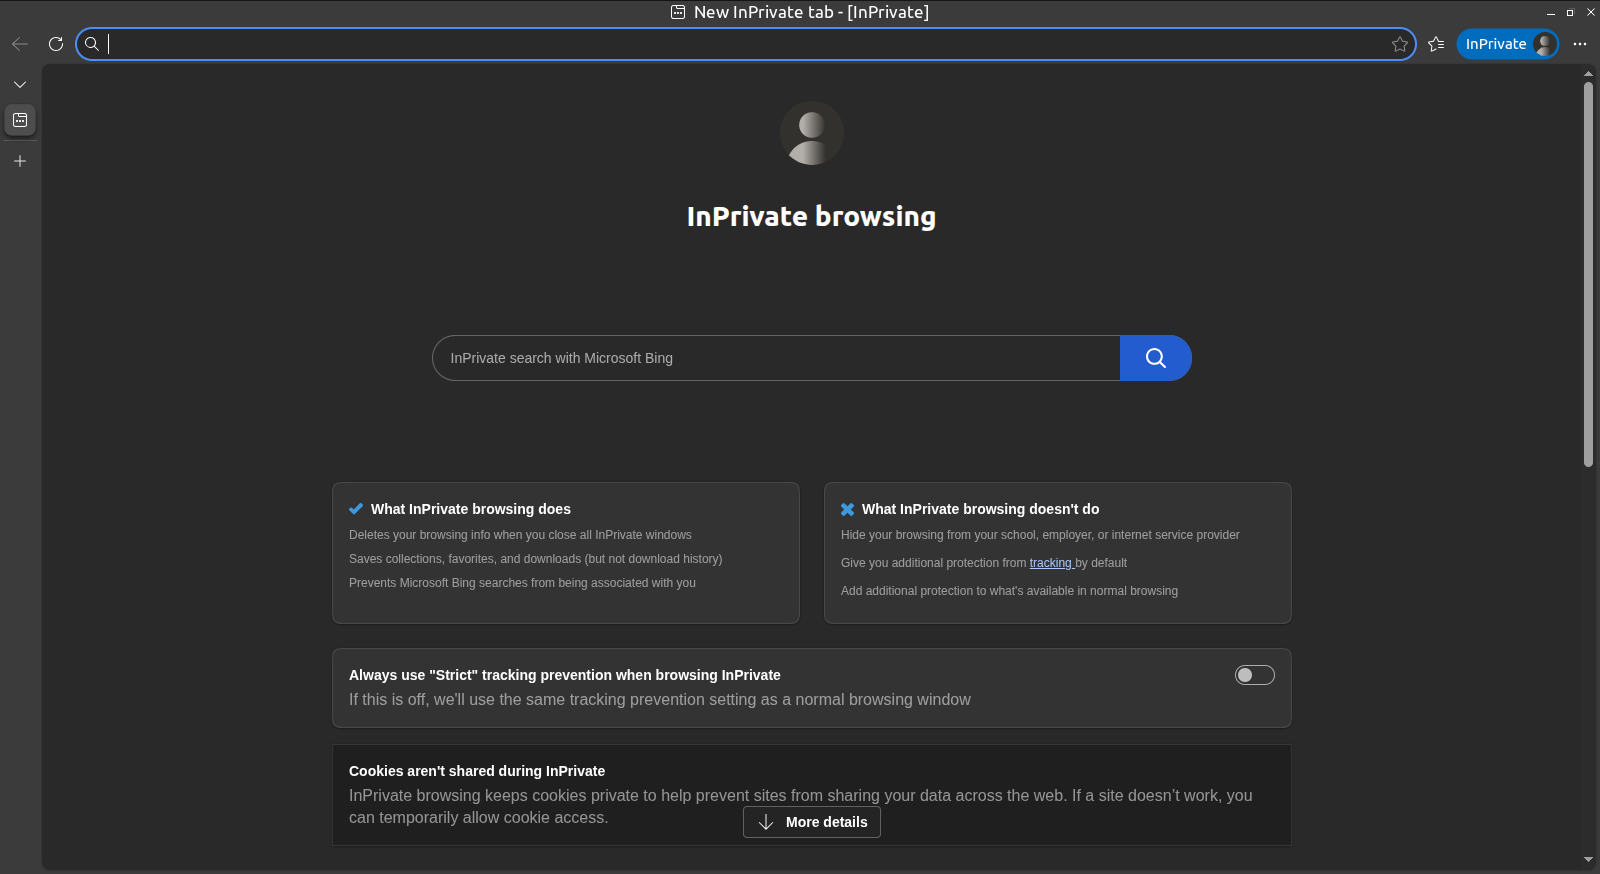
\includegraphics[width=0.75\linewidth]{images/navegacion-privada} 

}

\caption{Navegación privada navegador Microsoft-edge.}\label{fig:unnamed-chunk-4}
\end{figure}

Sin embargo, es importante comprender sus limitaciones. La navegación privada mejora la privacidad en el dispositivo que estás utilizando, pero no te convierte en una persona anónima en Internet. Tu actividad puede seguir siendo visible para los sitios web que visitas, los servicios en los que inicias sesión, tu proveedor de Internet, tu empresa, tu centro educativo o el administrador de la red desde la que te conectas.

Además, si accedes a servicios como Google, Microsoft, Facebook, Instagram, X o cualquier otra plataforma mediante tu cuenta personal, la actividad realizada podrá seguir asociándose a tu perfil aunque estés utilizando una ventana de navegación privada.

También debes tener en cuenta que este modo no protege frente a programas maliciosos, ataques de phishing ni técnicas avanzadas de seguimiento utilizadas por algunos sitios web, como la huella digital del navegador (browser fingerprinting), que intenta identificar tu dispositivo mediante sus características técnicas.

No es lo mismo navegar de forma privada que navegar de forma anónima. Para aumentar el anonimato en Internet se requieren herramientas y medidas adicionales, como la red \href{https://www.torproject.org/}{TOR} y otras soluciones específicas orientadas a proteger la identidad y dificultar el rastreo de la actividad en línea.

El uso de la navegación privada puede resultar especialmente útil en situaciones como las siguientes:

\begin{itemize}
\item
  Utilizar un ordenador compartido o de terceros.
\item
  Acceder temporalmente a una cuenta sin que la sesión quede almacenada en el navegador.
\item
  Realizar búsquedas o consultas que no deseas que aparezcan posteriormente en el historial local del dispositivo.
\item
  Comparar resultados o contenidos web reduciendo la influencia de las cookies almacenadas previamente.
\end{itemize}

Por otra parte, algunos navegadores y buscadores incorporan funciones de protección de la privacidad de forma predeterminada, incluyendo el bloqueo de rastreadores y técnicas de seguimiento. Entre ellos se encuentran \href{https://www.epicbrowser.com/}{Epic}, \href{https://brave.com/es/}{Brave} o buscadores como \href{https://duckduckgo.com/}{DuckDuckGo}

Recuerda que la navegación privada es una herramienta útil para proteger tu privacidad local, pero no debe considerarse una solución completa para preservar tu anonimato o impedir toda recopilación de datos en Internet.

\section{VPN (Red privada virtual)}\label{vpn-red-privada-virtual}

Otra forma de reforzar tu privacidad en Internet es utilizar una VPN (siglas de Virtual Private Network o red privada virtual) \citep{XATAKA-vpn}.

Una VPN crea una conexión cifrada entre tu dispositivo y un servidor gestionado por el proveedor de la VPN. De esta forma, tu proveedor de acceso a Internet o las personas conectadas a la misma red (por ejemplo, en una red Wi-Fi pública) tienen más dificultades para conocer qué información intercambias con los sitios web que visitas.

Además, los servicios de Internet verán la dirección IP del servidor VPN en lugar de la tuya, lo que puede ayudar a ocultar tu ubicación aproximada y permitir el acceso a contenidos o servicios disponibles únicamente en determinados países o regiones.

Sin embargo, una VPN no proporciona anonimato total ni te protege frente a todas las amenazas. El proveedor de la VPN puede tener acceso a determinados datos de tu conexión, por lo que es importante elegir servicios de confianza, revisar sus políticas de privacidad y desconfiar de aplicaciones gratuitas de origen desconocido.

Las VPN suelen ofrecerse mediante aplicaciones específicas para ordenadores y dispositivos móviles, aunque algunos navegadores incorporan funciones similares, como el navegador \href{https://www.opera.com/es}{OPERA} que lo trae por defecto. Una vez activada, la VPN cifra el tráfico entre tu dispositivo y el servidor VPN, dificultando que terceros intercepten o supervisen tu actividad en la red.

Recuerda que una VPN es un herramienta más como medida de privacidad, pero no sustituye las buenas prácticas de ciberseguridad. Aunque utilices una VPN, debes seguir prestando atención a posibles fraudes, correos electrónicos sospechosos, páginas web falsas, aplicaciones maliciosas o contenidos manipulados mediante inteligencia artificial, como mensajes automatizados o deepfakes utilizados para engañar a las personas.

\section{Cookies}\label{cookies}

Una cookie es un fichero que guarda nuestro navegador, donde se almacenan pequeñas cantidades de datos, de manera que el sitio web puede consultar la actividad previa del navegador.

Su propósito principal es identificar al usuario almacenando su historial de actividad de un sitio web específico, de manera que se le pueda ofrecer el contenido más apropiado según sus hábitos. Esto quiere decir que cada vez que visitas una página web por primera vez, se guarda una cookie en el navegador con un poco de información. Luego, cuando visitas nuevamente la misma página, el servidor pide la misma cookie para arreglar la configuración del sitio y hacer la visita del usuario tan personalizada como sea posible \citep{cookies-navegador}.

Existe la opción de navegar sin cookies gracias a las sesiones privadas que tienen los distintos navegadores, como has podido ver en el apartado anterior. De esta forma no se almacenará ningún tipo de información en tu ordenador cuando navegues en una web y del mismo modo tampoco recordará nada después al volver a navegar de nuevo.

Es importante que con frecuencia elimines las cookies, ahora que sabes que manejan información privada y además ocupan espacio en tu dispositivo. Existen dos formas manuales de hacerlo. La primera de ellas es desde el menú de opciones del propio navegador y la otra es con un software específico para tal cometido, como por ejemplo \href{https://www.ccleaner.com/es-es}{Ccleaner}. Pero si quieres automatizar esta tarea, prácticamente todos los navegadores disponen de una configuración para que una vez cierres el navegador se realice una limpieza de manera automática. La siguiente imagen te muestra la opción que debes buscar en el navegador Google Chrome, para ello ve al Menu del navegador, entra en Configuracíón, luego Privacidad y seguridad, a continuación, Cookies y finalmente Borrar las cookies y los datos de sitios al salir de Chrome, pero debes tener en cuenta que las ubicaciones pueden variar con las actualizaciones. Si usas otro navegador puede ser que varíe la ruta de acceso, pero a grandes rasgos suelen ser muy parecidas y también se acceden a ellas a través del menú de opciones.

\begin{figure}

{\centering \includegraphics[width=0.75\linewidth]{images/borrado-cookies-cierre-navegador} 

}

\caption{Eliminar cookies automáticamente al cerrar Google Chrome.}\label{fig:unnamed-chunk-5}
\end{figure}

Por otro lado si quieres deshacerte de la incómoda notificación de cookies de las web, puedes instalar en el navegador el plugin \href{https://www.i-dont-care-about-cookies.eu/}{I don't care about cookies}.

Si quieres más información detallada sobre las cookies visita este enlace \href{https://www.osi.es/es/actualidad/blog/2019/09/11/por-que-borrar-las-cookies-del-navegador}{por qué borrar las cookies} y este otro \href{https://www.osi.es/es/actualidad/blog/2018/07/18/entre-cookies-y-privacidad}{tipos de cookies, configuración y consejos} de la Oficina de Seguridad del Internauta donde las analizan con más detalle.

Al hilo de las cookies debes saber que estas no son la única manera que existe de tracear nuestra actividad en internet y que hay técnicas más sofisiticadas. Estas técnicas son conocidas como Fingerprinting y hacen un rastreo de tu huella digital. Por lo tanto, el fingersprinting es una técnica que permite obtener información de una persona o empresa a través de los sistemas informáticos.

Si quieres profundizar más en este tema te recomiendo que visites el siguiente enlace \href{https://protecciondatos-lopd.com/empresas/fingerprinting-que-es/}{¿Qué es el fingerprinting?}.

Para que te hagas una idea de lo que implica una política de cookies, a continuación tienes un ejemplo de los tipos de cookies y sus funciones.

Política de Cookies:
El portal web ``x'' hace uso de cookies. Con su aceptación de la presente política concede su permiso para obtener datos estadísticos de su navegación en esta web, en cumplimiento del Real Decreto-ley 13/2012. Si continúa navegando consideramos que acepta el uso de cookies.

¿Qué son las cookies?
Las cookies son archivos que las páginas web almacenan en el navegador del usuario que las visita, necesarias para aportar a la navegación web ventajas en la prestación de servicios interactivos.

Tipos posibles de cookies:

\begin{itemize}
\item
  Cookies de sesión: Son un tipo de cookies diseñadas para recabar y almacenar datos mientras el usuario accede a una página web, y no queda registrada en el disco del usuario.
\item
  Cookies persistentes: Son un tipo de cookies en el que los datos siguen almacenados en el terminal y pueden ser accedidos y tratados durante un periodo definido por el responsable de la cookie, y que puede ir de unos minutos a varios años.
\item
  Propias: son cookies generadas por la propia página web que se está visitando.
\item
  De terceros: son cookies que se reciben al navegar por esa página web, pero que han sido generadas por un tercer servicio que se encuentra hospedado en ella.
\end{itemize}

Fines de las cookies:

\begin{itemize}
\item
  Fines técnicos: Son necesarias para el funcionamiento de la página web. Son las denominadas también estrictamente necesarias. Hacen posible el control de tráfico desde el servidor a múltiples usuarios a la vez, la identificación y el acceso como usuario del sistema, etc.
\item
  Personalización: Hacen posible que cada usuario pueda configurar aspectos como el lenguaje en el que desea ver la página web o la configuración regional.
\item
  Análisis o rendimiento: Permiten medir el número de visitas y criterios de navegación de diferentes áreas de la web de forma anónima.
\item
  Publicidad: Permiten implementar parámetros de eficiencia en la publicidad ofrecida en las páginas web.
\item
  Publicidad comportamental: Permiten implementar parámetros de eficiencia en la publicidad ofrecida en las páginas web, basados en información sobre el comportamiento de los usuarios.
\end{itemize}

Uso de Cookies:

La web ``x'' SOLO utiliza las siguientes COOKIES: Cookies de tipo comportamental para el almacenamiento de sesión y de caché para mejorar su experiencia.

\begin{itemize}
\item
  Cookies de análisis: Son aquéllas que permiten al responsable de las mismas, el seguimiento y análisis del comportamiento de los usuarios de los sitios web a los que están vinculadas. La información recogida mediante este tipo de cookies se utiliza en la medición de la actividad de los sitios web, aplicación o plataforma y para la elaboración de perfiles de navegación de los usuarios de dichos sitios, aplicaciones y plataformas, con el fin de introducir mejoras en función del análisis de los datos de uso que hacen los usuarios del servicio.
\item
  Cookies publicitarias: Son aquéllas que permiten la gestión, de la forma más eficaz posible, de los espacios publicitarios que, en su caso, el editor haya incluido en una página web, aplicación o plataforma desde la que presta el servicio solicitado en base a criterios como el contenido editado o la frecuencia en la que se muestran los anuncios.
\item
  Cookies de publicidad comportamental: Son aquéllas que permiten la gestión, de la forma más eficaz posible, de los espacios publicitarios que, en su caso, el editor haya incluido en una página web, aplicación o plataforma desde la que presta el servicio solicitado. Estas cookies almacenan información del comportamiento de los usuarios obtenida a través de la observación continuada de sus hábitos de navegación, lo que permite desarrollar un perfil específico para mostrar publicidad en función del mismo.
\item
  Estrictamente necesarias: Las Cookies estrictamente necesarias le permiten navegar por la página web y usar sus funciones esenciales.
\end{itemize}

Relacionado con las cookies también exite el ciberataque conocido como el secuestro de cookies que puedes leer en este artículo \href{https://www.incibe.es/ciudadania/blog/que-es-el-secuestro-de-cookies-de-sesion-y-como-puede-afectarte}{¿Qué es el secuestro de cookies de sesión y cómo puede afectarte?}

Además actualmente, muchas plataformas utilizan sistemas de inteligencia artificial para analizar la información obtenida mediante cookies, datos de navegación y otras técnicas de seguimiento. Esto les permite identificar patrones de comportamiento, predecir intereses y personalizar contenidos, recomendaciones o publicidad de forma cada vez más precisa. Por ello, es importante revisar periódicamente la configuración de privacidad de los servicios que utilizas y limitar, cuando sea posible, la recopilación de datos innecesarios.

\section{Permisos cámara, micrófono y localización.}\label{permisos-cuxe1mara-micruxf3fono-y-localizaciuxf3n.}

Una práctica muy saludable en el uso de la cámara o webCam e incluso el micrófono, es tenerla tapada cuando no la estés usando y si no fíjate en la foto que se muestra a continuación que le tomaron a Mark Zuckerberg.

\begin{figure}

{\centering \includegraphics[width=0.75\linewidth]{images/webca-mark-zuckerberg} 

}

\caption{WebCam y micrófono del ordenador tapados.}\label{fig:unnamed-chunk-6}
\end{figure}

Para tener el control total sobre las funcionalidades de cámara, micrófono y ubicación, debes establecer los permisos en la opción de Preguntar, lo verás más claramente en la imagen que se muestra más abajo. Para establecer estos parámetros existen dos maneras de hacerlo, uno de ellas es a través de las opciones que te da el menú de configuración del propio navegador, y para ello debes ir a Menú navegador, buscar Configuracíón, después Privacidad y seguridad, a continuación Configuración de sitios web y finalmente Permisos. Como ya se indicó en el caso de borrado de cookies automático, debes tener en cuenta que las ubicaciones pueden variar con las actualizaciones que reciba el navegador.

\begin{figure}

{\centering \includegraphics[width=0.75\linewidth]{images/ajuste-permisos} 

}

\caption{Ajustes permisos cámara, micrófono y ubicación desde el menú de opciones del navegador.}\label{fig:unnamed-chunk-7}
\end{figure}

Aunque estos permisos son los más importantes cuando navegas por internet, si te fijas en la figura 2.4 verás que no son los únicos y que entre éstos se encuentran los de notificaciones o los de ventanas emergentes entre otros.

La gestión de estos permisos puede realizarse desde la configuración del navegador. Aunque la ubicación exacta de las opciones puede variar según la versión utilizada, normalmente se encuentran en los apartados de Privacidad y seguridad o Configuración de sitios. Desde allí podrás revisar y modificar el acceso a la cámara, el micrófono, la ubicación, las notificaciones y otros elementos del dispositivo.

También es posible consultar y modificar los permisos de una página web concreta directamente desde la barra de direcciones del navegador. Al seleccionar el icono situado junto a la dirección web (candado u otro símbolo equivalente según el navegador), podrás comprobar qué permisos tiene concedidos ese sitio y modificarlos si lo consideras necesario.

Recuerda que el icono del candado únicamente indica que la comunicación con la página web está cifrada mediante HTTPS. No garantiza por sí solo que el sitio sea legítimo ni que todo su contenido sea seguro, por lo que siempre debes mantener una actitud crítica ante cualquier solicitud de información o permiso.

\begin{figure}

{\centering \includegraphics[width=0.75\linewidth]{images/ajuste-permisos-desde-navegador} 

}

\caption{Ajustes permisos cámara, micrófono y ubicación desde el candado de la barra de direcciones.}\label{fig:unnamed-chunk-8}
\end{figure}

Tampoco debes olvidar que con las aplicaciones móviles sucede lo mismo, y que puedes gestionarlos de igual manera desde ajustes del dispositivo. Visita los siguientes enlaces dependiendo de tu smartphone, \href{https://support.google.com/android/answer/9431959?hl=es}{cambiar los permisos de las aplicaciones en teléfonos Android} o \href{https://support.apple.com/es-es/guide/iphone/iph251e92810/ios}{controlar el acceso a la información en las apps en el iPhone}. Es recomendable revisarlos periódicamente y eliminar aquellos que ya no sean necesarios, aplicando el principio de conceder únicamente los permisos mínimos indispensables para cada aplicación.

En la actualidad, muchas aplicaciones incorporan funciones basadas en inteligencia artificial que pueden requerir acceso a la cámara, el micrófono, las fotografías, los vídeos o la ubicación. Antes de conceder estos permisos, revisa si son realmente necesarios para el funcionamiento de la aplicación y evita otorgar acceso permanente cuando no sea imprescindible.

\section{La nube}\label{la-nube}

El almacenamiento en la nube consiste en guardar información en servidores gestionados generalmente por terceros. Gracias a ello, puedes acceder a tus archivos desde distintos dispositivos y ubicaciones, siempre que dispongas de conexión a Internet y acceso al servicio donde se encuentran almacenados. De esta forma, ya no es necesario transportar físicamente los dispositivos donde guardas tu información. Algunos de estos servicios más conocidos son \href{https://www.google.com/intl/en_in/drive/}{Google drive}, \href{https://www.microsoft.com/en-us/microsoft-365/onedrive/online-cloud-storage}{One drive} o \href{https://www.dropbox.com/}{Dropbox} entre otros.

Antes de elegir un proveedor de almacenamiento en la nube, conviene que tengas en cuenta los siguientes aspectos:

\begin{itemize}
\item
  Dónde se almacenará tu información. Esto te permitirá conocer qué legislación se aplica y qué garantías de protección de datos existen en el país o región donde se encuentren los servidores.
\item
  Si la plataforma comparte información con terceros y con qué finalidad.
\item
  Si el acceso al servicio se realiza mediante una conexión segura (HTTPS).
\item
  Los mecanismos de cifrado utilizados para proteger la información almacenada y transmitida.
\item
  Sus políticas de privacidad y condiciones de uso.
\item
  Las condiciones relativas al uso de inteligencia artificial y al tratamiento automatizado de los datos almacenados.
\end{itemize}

Actualmente muchos servicios en la nube incorporan herramientas basadas en inteligencia artificial que permiten buscar información, resumir documentos, analizar imágenes o facilitar la organización de los contenidos. Estas funciones pueden resultar útiles, pero es recomendable revisar qué información pueden procesar, cómo se utiliza y si existe la posibilidad de limitar determinados tratamientos de datos.

Antes de subir información a la nube, valora su nivel de sensibilidad. Los documentos que contengan datos personales, financieros, sanitarios o información especialmente confidencial requieren mayores precauciones. En estos casos, puede ser recomendable cifrar los archivos antes de almacenarlos. Para ello puedes utilizar herramientas como \href{https://cryptomator.org/}{cryptomator}.

A la hora de compartir archivos o carpetas alojados en la nube, procura hacerlo únicamente con las personas necesarias y revisa cuidadosamente los permisos concedidos. Un enlace configurado incorrectamente o compartido públicamente puede permitir el acceso no autorizado a la información. También es aconsejable revisar periódicamente qué personas, dispositivos y aplicaciones mantienen acceso a tus datos.

Recuerda que la seguridad de tus archivos no depende únicamente del proveedor del servicio. Revisar regularmente la configuración de privacidad son medidas fundamentales para proteger tu información.

\section{Correo electrónico y apps de mensajería}\label{correo-electruxf3nico-y-apps-de-mensajeruxeda}

El correo electrónico sigue siendo una de las herramientas de comunicación digital más utilizadas. Sin embargo, no todos los proveedores ofrecen el mismo nivel de privacidad, seguridad o control sobre los datos. Dependiendo del servicio utilizado, parte de la información asociada a tus comunicaciones puede ser analizada para prestar determinadas funcionalidades o mejorar sus servicios.

Esto no tiene por qué ser un inconveniente si no envías información sensible, pero si no es el caso quizá preferirías usar un gestor de correos que sí te garantice una privacidad completa en tus envíos. De ser este tu caso puedes usar \href{https://protonmail.com/}{Protonmail}, \href{https://tutanota.com/es/}{Tutanota} o \href{https://www.fastmail.com}{Fastmail} que sí tienen en cuenta este aspecto, aunque no son los únicos. En el siguiente enlace tienes una lista de otras \href{https://blogthinkbig.com/alternativas-gratuitas-gmail-outlook-privacidad}{alternativas de emails privadas}.

Otra opción consiste en cifrar los mensajes antes de enviarlos mediante herramientas específicas de cifrado de correo electrónico. De esta forma, incluso si el mensaje fuera interceptado, su contenido no podría ser leído sin la clave correspondiente. Tienes otras herramientas para llevar a cabo este propósito en este artículo de \href{https://www.osi.es/es/actualidad/blog/2019/07/31/como-encriptar-y-proteger-tu-correo-electronico}{cómo encriptar y proteger tu correo electrónico}.

Otra alternativa de envío de correos cifrados, es el uso de la opción de correos confidenciales de Gmail. De esta manera el receptor necesitará un código para desbloquear el contenido del email que, recibirá a través de SMS en su smartphone. Más información en el siguiente enlace \href{https://support.google.com/mail/answer/7674059?hl=es&co=GENIE.Platform\%3DDesktop}{Enviar y abrir correos confidenciales}.

Si además quieres saber si tu cuenta de correo o tu número de teléfono han sido comprometidos, puedes saberlo a través de la siguiente plataforma \href{https://haveibeenpwned.com/}{haveibeenpwned}.

Con respecto a las aplicaciones de mensajería instantánea debes tener en cuenta que sucede lo mismo que con los correos electrónicos. A pesar que la mayoría de ellas, incluida la más popular de todas (WhatsApp) disponen de capas de privacidad que la hacen confiable, a veces no podemos estar totalmente seguros de no estar sometidos a un seguimiento por parte de éstas. Es por ello, que las aplicaciones como \href{https://telegram.org/}{telegram} y \href{https://signal.org/es/}{signal} nacen con el propósito de no inmiscuirse en el uso que haces de la aplicación.

Antes de elegir una aplicación de mensajería, es recomendable informarte sobre:

\begin{itemize}
\item
  Qué datos recopila la plataforma.
\item
  Qué metadatos conserva (por ejemplo, quién se comunica con quién o cuándo se producen las comunicaciones).
\item
  Si utiliza cifrado de extremo a extremo por defecto.
\item
  Cómo gestiona las copias de seguridad.
\item
  Qué políticas aplica respecto al tratamiento de datos y la privacidad.
\end{itemize}

Asimismo, algunas plataformas incorporan asistentes basados en inteligencia artificial capaces de resumir mensajes, redactar respuestas o buscar información en tus conversaciones. Aunque estas funciones pueden resultar útiles, conviene revisar las opciones de privacidad disponibles y comprender cómo se procesan los datos antes de utilizarlas con información sensible.

\section{Cifrado o encriptado de datos}\label{cifrado-o-encriptado-de-datos}

Mantener tus documentos simplemente organizados en carpetas no siempre es suficiente para proteger la información, especialmente cuando se trata de datos personales, financieros, laborales o cualquier otro contenido sensible. Si alguien obtiene acceso físico o remoto a tu dispositivo, podría intentar acceder a esa información. Por ello, una de las medidas más eficaces consiste en utilizar herramientas de cifrado o encriptado de datos.

El cifrado es un proceso que transforma la información en un formato ilegible para cualquier persona que no disponga de la clave o contraseña necesaria para acceder a ella. De esta forma, aunque un tercero consiga copiar los archivos, no podrá interpretar su contenido.

Una de las herramientas más conocidas para este fin es \href{https://cryptomator.org/}{Cryptomator}. Se trata de un software de código abierto que permite crear espacios cifrados donde almacenar archivos y carpetas de forma segura. Está disponible para Windows, macOS y Linux, además de contar con aplicaciones para dispositivos Android e iPhone.

Con Cryptomator puedes crear diferentes bóvedas cifradas, protegidas mediante una contraseña. Dentro de ellas podrás almacenar toda la información que desees proteger. Mientras la bóveda permanezca cerrada, los archivos estarán cifrados y no podrán ser leídos sin la contraseña correspondiente.

Es importante que utilices una contraseña robusta y que la conserves de forma segura. Si la olvidas, recuperar el acceso a la información puede resultar imposible.

Además del cifrado de archivos concretos, muchos sistemas operativos actuales incorporan opciones para cifrar completamente el dispositivo, lo que añade una capa adicional de protección frente a pérdidas, robos o accesos no autorizados. Pero esto es algo que veraś más adelante en la unidad \hyperref[gestiuxf3n-de-la-seguridad-en-equipos-fuxedsicos]{3 Gestión de la seguridad en equipos físicos}.

Otra práctica especialmente recomendable consiste en cifrar los archivos antes de almacenarlos en servicios de nube. De esta forma, aunque los datos se encuentren alojados en servidores de terceros, solo podrán ser leídos por quienes dispongan de la contraseña de descifrado.

La creciente utilización de herramientas basadas en inteligencia artificial hace aún más importante proteger adecuadamente la información sensible. Documentos personales, conversaciones, informes o datos utilizados en servicios digitales pueden contener información valiosa que no debería quedar expuesta ante accesos no autorizados. El cifrado ayuda a reducir estos riesgos y proporciona una capa adicional de control sobre tus datos.

Recuerda que ninguna medida de privacidad es absoluta. El cifrado es una herramienta muy eficaz, pero no sustituye el resto de medidas para aportar robustez a tu privacidad.

\section{He decidido vender o donar mi dispositivo}\label{he-decidido-vender-o-donar-mi-dispositivo}

Si estás pensando en vender, regalar o donar un dispositivo que haya almacenado información personal, como un ordenador, un teléfono móvil, una tableta, un disco duro externo o una memoria USB, es importante que elimines correctamente todos los datos antes de entregarlo a otra persona.

Muchas personas creen que formatear un dispositivo es suficiente para borrar su contenido. Sin embargo, dependiendo del tipo de almacenamiento y del método utilizado, parte de la información podría llegar a recuperarse mediante herramientas especializadas. Por lo que, con software avanzado y específico los ciberdelicuentes podrían recuperar todo el contenido \citep{XATAKA-borrado-almacenamiento}.

Antes de realizar cualquier proceso de borrado, asegúrate de hacer una copia de seguridad de los datos que desees conservar. Después:

\begin{itemize}
\item
  Cierra sesión en todas tus cuentas y servicios.
\item
  Desvincula el dispositivo de plataformas en la nube.
\item
  Elimina las cuentas configuradas en el equipo.
\item
  Borra las contraseñas almacenadas.
\item
  Restablece el dispositivo a sus valores de fábrica cuando exista esta opción.
\end{itemize}

En muchos dispositivos modernos, especialmente teléfonos inteligentes y equipos con almacenamiento cifrado, el restablecimiento completo combinado con el cifrado previo de los datos proporciona una protección muy eficaz frente a la recuperación de información.

Para discos duros, memorias USB u otros soportes de almacenamiento, también puedes utilizar herramientas específicas de borrado seguro que sobrescriben los datos o aplican procedimientos diseñados para impedir su recuperación.

La eliminación adecuada de la información es hoy más importante que nunca. Fotografías, vídeos, grabaciones de voz, correos electrónicos, documentos o conversaciones almacenadas en un dispositivo pueden contener información suficiente para realizar fraudes, suplantaciones de identidad o ataques de ingeniería social. Además, los avances en inteligencia artificial permiten analizar grandes cantidades de datos y generar contenidos falsos muy convincentes a partir de información obtenida de dispositivos mal gestionados.

Por este motivo, antes de desprenderte de cualquier dispositivo, dedica unos minutos a asegurarte de que no contiene información personal recuperable. Esta sencilla medida puede evitar problemas de privacidad y seguridad tanto para ti como para las personas relacionadas contigo.

Algunas herramientas de borrado seguro son:

\begin{itemize}
\item
  \href{https://www.diskwipe.org/download.php}{Disk wipe} (borrado seguro de discos y particiones).
\item
  \href{https://www.killdisk.com/eraser.html}{Active@ KillDisk} (borrado seguro de HDD, SSD y memorias USB).
\item
  Herramientas oficiales del fabricante del SSD (por ejemplo, Samsung Magician para SSD Samsung).
\end{itemize}

En casos en los que el dispositivo haya almacenado información extremadamente sensible y no vaya a reutilizarse, puede ser recomendable destruir físicamente el soporte de almacenamiento para impedir cualquier intento de recuperación de datos.

Si quieres más recomendaciones sobre como actuar en este supuesto, te recomiendo que leas la siguiente entrada \href{https://www.osi.es/es/actualidad/blog/2019/10/09/sabias-que-2-de-cada-5-dispositivos-vendidos-contienen-informacion}{¿Sabías que 2 de cada 5 dispositivos vendidos contienen información personal?}.

\section{Inteligencia Artificial y privacidad}\label{inteligencia-artificial-y-privacidad}

La irrupción de las herramientas de Inteligencia Artificial (IA) generativa, como los chats inteligentes, asistentes de búsqueda o creadores de contenido, ha cambiado las reglas de juego de la privacidad. A diferencia del software tradicional, estos sistemas se ``alimentan'' y entrenan continuamente con la información que introducimos en ellos mediante prompts. Esto significa que cualquier dato personal, documento laboral o fotografía que compartamos con una IA puede pasar a formar parte de su base de conocimiento global, con el riesgo de ser expuesto a terceros en futuras respuestas.

Para interactuar con estas tecnologías de forma responsable y proteger nuestra identidad digital, es imprescindible adoptar las siguientes medidas:

\begin{itemize}
\item
  Desactivar el entrenamiento, historial o usa conversación temporal: Se debe revisar a fondo la configuración de la cuenta en la plataforma de IA para activar las opciones que impiden que las conversaciones se almacenen en sus servidores o se utilicen para entrenar a sus futuros modelos de lenguaje.
\item
  Anonimización de datos (prompts limpios): Antes de enviar cualquier texto a una IA, se debe eliminar todo dato identificativo. Si se necesita resumir un documento o redactar un correo, es necesario sustituir los nombres reales, direcciones, teléfonos o datos fiscales por términos genéricos (como ``Persona A'' o ``Empresa X'').
\item
  Cuidado con el contenido multimedia y biométrico: Evitar subir fotografías personales, archivos de voz o vídeos a herramientas de IA de dudosa procedencia para modificar rostros o clonar voces, ya que se están entregando patrones de identidad únicos a servidores externos con políticas de retención de datos ambiguas.
\item
  Alternativas locales: Siempre que sea posible, se debe priorizar el uso de modelos de IA que se ejecuten de manera local en el propio dispositivo (sin enviar datos a la nube) o utilizar servicios corporativos que garanticen contractualmente la privacidad y el borrado inmediato de la información compartida.
\end{itemize}

\section{Dispositivos del hogar conectado (IoT) y el rastreo doméstico}\label{dispositivos-del-hogar-conectado-iot-y-el-rastreo-domuxe9stico}

La proliferación de electrodomésticos inteligentes, televisores con conexión a internet, altavoces con asistente de voz o básculas digitales ha convertido el hogar en un entorno de recolección de datos masiva. Estos dispositivos del Internet de las Cosas (IoT) no solo interactúan con nosotros, sino que monitorizan de forma constante nuestros hábitos más íntimos: horarios de sueño, pautas de consumo, mapas del interior de la vivienda e incluso conversaciones ambientales. Para evitar que el ecosistema domótico se transforme en una herramienta de espionaje comercial y salvaguardar la privacidad del hogar, se deben adoptar las siguientes medidas:

\begin{itemize}
\item
  Gestionar el historial de voz y grabaciones: En los altavoces inteligentes y pantallas conectadas, es necesario acceder a la configuración de privacidad de la cuenta (como Google, Amazon o Apple) para revisar, borrar y desactivar el almacenamiento permanente de los comandos de voz y las muestras de audio capturadas.
\item
  Limitar la telemetría y el envío de diagnósticos: Durante la configuración de cualquier aparato (especialmente Smart TVs y robots aspiradores), se deben desmarcar sistemáticamente las casillas de ``compartir datos de uso'', ``informes de diagnóstico'' o ``experiencia de usuario'', las cuales envían información sobre nuestros hábitos de consumo a los fabricantes.
\item
  Capar la publicidad personalizada en Smart TVs: Las televisiones actuales rastrean el contenido exacto que ves en pantalla (tecnología ACR o Reconocimiento Automático de Contenido) para enviarte anuncios dirigidos. Es imprescindible buscar y desactivar esta opción en los menús de privacidad del televisor.
\item
  Revisar los permisos de las aplicaciones de gestión: Los dispositivos IoT se controlan mediante apps móviles que a menudo exigen accesos abusivos. Se debe retirar el permiso de localización, acceso a la agenda de contactos o a la galería de fotos si la aplicación del aparato (por ejemplo, una bombilla o un purificador de aire) no los necesita para su funcionamiento básico.
\item
  Evaluar la necesidad de conexión: Antes de conectar un nuevo electrodoméstico a la red Wi-Fi, conviene valorar si esa conexión aporta un valor real. Si un dispositivo (como un frigorífico o una cafetera) funciona perfectamente sin internet, mantenerlo ``desconectado'' es la política de privacidad más radical y efectiva.
\end{itemize}

\chapter{Gestión de la seguridad en equipos físicos}\label{gestiuxf3n-de-la-seguridad-en-equipos-fuxedsicos}

\section{Gestionar la seguridad en los equipos}\label{gestionar-la-seguridad-en-los-equipos}

Para proteger tus dispositivos, como el ordenador, la tablet, el smartphone o el router, es fundamental mantener unas medidas de seguridad adecuadas. Estas medidas te ayudarán a prevenir accesos no autorizados, infecciones por programas maliciosos, pérdidas de información y otros incidentes que pueden afectar tanto a tus datos como a tu privacidad.

En la actualidad, además de las amenazas tradicionales, han surgido nuevos riesgos asociados al uso de servicios digitales e inteligencia artificial, como aplicaciones fraudulentas, intentos de engaño más sofisticados o el uso indebido de información personal. Por ello, resulta cada vez más importante adoptar hábitos de seguridad adecuados y mantener los dispositivos correctamente configurados y actualizados.

A lo largo de esta unidad conocerás las principales medidas y precauciones que debes aplicar para mantener tus equipos y tu información protegidos frente a los ciberataques y otros riesgos digitales.

\section{Cuentas de usuario en equipos locales y dispositivos móviles}\label{cuentas-de-usuario-en-equipos-locales-y-dispositivos-muxf3viles}

Una cuenta de usuario es el conjunto de información perteneciente a un usuario concreto. De esta forma indica al sistema operativo los archivos y carpetas a los que dicho usuario tiene acceso, así como la posibilidad de realizar cambios y configuraciones personales.

Las recomendaciones de seguridad que se presentan a continuación son aplicables tanto a ordenadores como a dispositivos móviles, tablets, relojes inteligentes y otros equipos conectados.

Cada persona debería utilizar su propia cuenta de usuario y evitar compartirla con terceros. Cuando varias personas utilizan un mismo dispositivo, es recomendable crear cuentas independientes para cada una de ellas. De este modo, cada usuario dispone de su propio espacio de trabajo y sus datos permanecen separados.

Si tu equipo es compartido con varias personas, puede resultarte útil crear diferentes cuentas con distintos niveles de permisos. Una gestión inadecuada de estas cuentas puede provocar situaciones como:

\begin{itemize}
\item
  Acceso no autorizado a documentos, fotografías, vídeos u otra información personal.
\item
  Modificación o eliminación accidental o intencionada de archivos.
\item
  Cambios en la configuración de seguridad del sistema, como la desactivación del antivirus o del cortafuegos.
\item
  Acceso a servicios personales utilizando sesiones abiertas o credenciales almacenadas.
\end{itemize}

Muchos dispositivos actuales permiten vincular la cuenta local a servicios en línea, como cuentas Microsoft, Apple o Google. Estas cuentas suelen proporcionar acceso a correo electrónico, almacenamiento en la nube, copias de seguridad y otros servicios. Por ello, protegerlas adecuadamente es especialmente importante.

Puedes gestionar cuentas de usuarios en \href{https://support.microsoft.com/es-es/windows/administrar-cuentas-de-usuario-en-windows-104dc19f-6430-4b49-6a2b-e4dbd1dcdf32}{administrar cuentas de usuario en Windows} y en \href{https://support.apple.com/es-es/guide/mac-help/mchl3e281fc9/mac}{añadir una cuenta de usuario Mac} lo que te permitirá crear tantas cuentas de usuarios como sean necesarias.

\begin{figure}

{\centering \includegraphics[width=0.75\linewidth]{images/cuenta-usuario-windows-10} 

}

\caption{Cuenta de usuario Windows 10.}\label{fig:unnamed-chunk-9}
\end{figure}

Existen diferentes tipos de cuentas de usuario:

\begin{itemize}
\item
  Cuenta estándar o limitada: es la recomendada para el uso diario del dispositivo.
\item
  Cuenta de administrador: dispone de permisos avanzados para instalar programas, modificar configuraciones críticas o gestionar otras cuentas. Debe utilizarse únicamente cuando sea necesario realizar estas tareas.
\item
  Cuentas de invitado: se usan principalmente por personas que necesitan usar temporalmente el equipo y no disponen de otra cuenta.
\end{itemize}

Es también, recomendable bloquear la pantalla cuando te ausentes del equipo y configurar el bloqueo automático tras un periodo de inactividad.

\section{Router}\label{router}

El router es el dispositivo que proporciona conectividad entre tu red doméstica e Internet. Su función principal consiste en dirigir el tráfico de datos entre diferentes redes y, habitualmente, ofrecer acceso a la red inalámbrica (Wi-Fi) para tus dispositivos.

Para proteger tu red Wi-Fi, los routers incorporan distintos estándares de seguridad y cifrado que impiden que personas no autorizadas accedan a la conexión o a los dispositivos conectados.

Los principales estándares de seguridad Wi-Fi son:

\begin{itemize}
\tightlist
\item
  \href{https://es.wikipedia.org/wiki/Wired_Equivalent_Privacy}{WEP} (Wired Equivalent Privacy). Actualmente se considera inseguro y no debe utilizarse.
\item
  \href{https://es.wikipedia.org/wiki/Wi-Fi_Protected_Access}{WPA} (Wi-Fi Protected Access). Ha quedado obsoleto y tampoco se recomienda.
\item
  \href{https://es.wikipedia.org/wiki/WPA2}{WPA2} (Wi-Fi Protected Access 2). Sigue siendo seguro cuando se utiliza con cifrado AES y una contraseña robusta.
\item
  \href{https://es.wikipedia.org/wiki/WPA3}{WPA3} (Wi-Fi Protected Access 3). Es el estándar más seguro actualmente disponible para redes domésticas y el que se recomienda utilizar siempre que sea compatible con tus dispositivos.
\end{itemize}

Si tu router lo permite, configura la red con WPA3. En caso contrario, utiliza WPA2 con una contraseña larga, única y difícil de adivinar.

Es importante cambiar la contraseña Wi-Fi que viene configurada por defecto y utilizar una clave robusta. Cuanto más larga sea la contraseña, mayor será la dificultad para que pueda ser descubierta mediante ataques automatizados. Para una contraseña robusta pásate por la unidad \hyperref[gestiuxf3n-de-la-seguridad-en-la-red]{4 Gestión de la seguridad en la red}.

También es recomendable modificar el nombre de la red Wi-Fi (SSID) que trae el router de fábrica. Evita utilizar datos personales o información que pueda revelar el operador, el modelo del equipo o la identidad del propietario de la red.

De igual modo, cambia la contraseña de administración del router para impedir que terceros puedan acceder a su configuración. Utiliza una contraseña distinta de la empleada para la red Wi-Fi.

Otra medida recomendable es desactivar la función WPS (Wi-Fi Protected Setup) si no la utilizas. Esta característica facilita la conexión de nuevos dispositivos mediante un botón físico o un código PIN, pero ha presentado vulnerabilidades de seguridad en algunos modelos de router.

Mantén actualizado el firmware del router. Los fabricantes publican periódicamente actualizaciones que corrigen errores y vulnerabilidades de seguridad que podrían ser aprovechadas por atacantes.

Si tu router dispone de una red de invitados, utilízala para conectar dispositivos de visitas o dispositivos inteligentes del hogar (IoT), como cámaras, asistentes de voz o enchufes inteligentes. De este modo reduces el impacto de una posible intrusión.

También es aconsejable revisar periódicamente la lista de dispositivos conectados para detectar accesos no autorizados y desactivar la administración remota del router cuando no sea necesaria.

Algunos routers permiten configurar filtros basados en direcciones \href{https://es.wikipedia.org/wiki/Filtrado_MAC}{MAC} (Media Access Control) para autorizar únicamente determinados dispositivos. Aunque esta medida de filtrado MAC puede ayudar a gestionar los equipos conectados, no debe considerarse una protección de seguridad eficaz por sí sola, ya que estas direcciones pueden ser suplantadas.

Para realizar cualquiera de estas configuraciones necesitarás acceder al panel de administración del router. La dirección de acceso suele encontrarse en una etiqueta situada en el propio dispositivo, en la documentación del fabricante o facilitada por tu operador de Internet.

Visita el siguiente enlace para conocer las \href{https://www.incibe.es/ciudadania/formacion/infografias/principales-configuraciones-del-router}{principales configuraciones del router}.

\section{Actualizaciones}\label{actualizaciones}

Las actualizaciones son modificaciones que los fabricantes y desarrolladores publican para corregir errores, solucionar vulnerabilidades de seguridad, mejorar el funcionamiento de los dispositivos o incorporar nuevas características. Estas actualizaciones pueden afectar tanto al sistema operativo como a las aplicaciones, navegadores, antivirus o al firmware de determinados dispositivos.

Las actualizaciones de seguridad, también conocidas como parches, son correcciones desarrolladas por fabricantes y desarrolladores para solucionar vulnerabilidades, errores o problemas detectados en sistemas operativos, aplicaciones y otros componentes informáticos.

Además de corregir fallos de seguridad, las actualizaciones pueden incorporar nuevas funcionalidades, mejorar el rendimiento, aumentar la estabilidad del sistema, reforzar la privacidad o mejorar la compatibilidad con otros dispositivos y servicios.

Mantener tus dispositivos actualizados es una de las medidas de seguridad más importantes. Cuando un fabricante publica una actualización que corrige una vulnerabilidad, los ciberdelincuentes pueden intentar aprovechar ese fallo en aquellos equipos que todavía no han sido actualizados. Por este motivo, es recomendable instalar las actualizaciones tan pronto como estén disponibles.

Siempre que sea posible, activa las actualizaciones automáticas. De esta forma recibirás las correcciones de seguridad sin necesidad de realizar ninguna acción manual.

Las actualizaciones no afectan únicamente a los ordenadores y teléfonos móviles. También deben mantenerse actualizados los navegadores web, aplicaciones, antivirus, routers, televisores inteligentes, cámaras conectadas a Internet, asistentes de voz y cualquier otro dispositivo conectado a la red.

En ocasiones pueden existir vulnerabilidades para las que todavía no se ha publicado una solución. Estas se conocen como vulnerabilidades de día cero (zero-day). Cuando el fabricante publica una corrección, instalarla rápidamente ayuda a reducir el riesgo de que el dispositivo pueda verse comprometido.

La evolución de la inteligencia artificial está permitiendo a los fabricantes detectar y corregir problemas con mayor rapidez, pero también facilita que los atacantes automaticen la búsqueda y explotación de vulnerabilidades. Por ello, mantener todos los dispositivos y programas actualizados sigue siendo una de las medidas más eficaces para proteger tu información y tu privacidad.

La principal función de las actualizaciones es mejorar la seguridad, la estabilidad y la funcionalidad de los sistemas y aplicaciones, contribuyendo a reducir los riesgos asociados al uso de las tecnologías digitales.

\section{Antivirus, antimalware y cortafuegos}\label{antivirus-antimalware-y-cortafuegos}

Existen diferentes herramientas de seguridad diseñadas para proteger tus dispositivos frente a amenazas informáticas. Aunque a menudo se utilizan como sinónimos, cumplen funciones distintas y complementarias. Actualmente muchas soluciones de seguridad integran varias de estas funciones en un único producto.

La mayoría de estas herramientas pueden encontrarse en versiones gratuitas y de pago, con diferentes niveles de protección y funcionalidades.

\begin{itemize}
\item
  Antivirus y antimalware: Son programas diseñados para detectar, bloquear y eliminar software malicioso (malware), como virus, troyanos, ransomware, spyware o programas potencialmente no deseados. Las soluciones modernas combinan diferentes técnicas de detección para identificar tanto amenazas conocidas como comportamientos sospechosos que puedan indicar un ataque. Algunos de ellos \href{https://www.avira.com/es}{Avira}, \href{https://www.avast.com/es-es/index\#pc}{Avast}, \href{https://www.avg.com/es-es/homepage\#pc}{AVG}.
\item
  Firewall o cortafuegos: Es un mecanismo de seguridad que controla las comunicaciones entre tu dispositivo e Internet o entre diferentes redes. Su función es permitir o bloquear conexiones según unas reglas establecidas, evitando accesos no autorizados. Los principales sistemas operativos actuales incorporan cortafuegos integrados que proporcionan un nivel adecuado de protección para la mayoría de usuarios. El \href{https://en.wikipedia.org/wiki/Windows_Firewall}{firewall} más conocido es el Windows.
\end{itemize}

En la actualidad, muchas herramientas de seguridad incorporan tecnologías basadas en inteligencia artificial y aprendizaje automático para detectar amenazas nuevas o desconocidas. Sin embargo, los ciberdelincuentes también utilizan estas tecnologías para desarrollar ataques más sofisticados, por lo que ninguna solución de seguridad garantiza una protección absoluta.

Antes de instalar cualquier herramienta de seguridad, infórmate sobre las opciones disponibles y descárgalas siempre desde la página web oficial del fabricante o desde tiendas de aplicaciones legítimas. Desconfía de los programas que prometen eliminar amenazas de forma milagrosa o que muestran alertas alarmistas para inducirte a instalarlos.

Para la mayoría de usuarios domésticos, las soluciones de seguridad integradas en los sistemas operativos modernos ofrecen un nivel de protección adecuado siempre que se mantengan actualizadas.

Cabe destacar que Windows incorpora de forma nativa Microsoft Defender Antivirus, una solución de seguridad que incluye protección frente a malware, análisis en tiempo real y otras funciones de seguridad integradas en el sistema operativo. Del mismo modo, los dispositivos de Apple incorporan mecanismos de protección integrados, como el control de aplicaciones, la protección frente a software malicioso y actualizaciones de seguridad distribuidas directamente por el fabricante.

Además de las soluciones de seguridad instaladas en el dispositivo, existen herramientas online como \href{https://www.virustotal.com/gui/}{Virus Total} que permiten analizar archivos y enlaces sospechosos antes de abrirlos.

\section{Copias de seguridad}\label{copias-de-seguridad}

Una copia de seguridad o backup en informática es una copia de los datos originales que se realiza con el fin de disponer de un medio para recuperarlos en caso de su pérdida. Las copias de seguridad son útiles ante distintos eventos y usos, como por ejemplo, recuperar los sistemas informáticos o datos de una posible catástrofe informática, natural o intencionada, restaurar una pequeña cantidad de archivos que pueden haberse eliminado accidentalmente, corrompido o infectado por un virus informático u otras posibles causas \citep{WIKI-copias-seguridad}.

Actualmente las copias de seguridad son una de las medidas de protección más importantes frente al ransomware, un tipo de malware que puede cifrar tus archivos e impedirte acceder a ellos.

Simplificando el sistema de copias de seguridad que en algunas ocasiones puede llegar a ser complejo, están los siguiente:

\begin{itemize}
\item
  Completas: Del sistema operativo completo, de esta forma al restaurar la copia, dispondremos de nuevo de toda la configuración a nivel de S.O., software instalado, carpetas y archivos. Para este cometido vamos a necesitar de programas de terceros, algunos de ellos con versiones gratuitas y de pago, ejemplo de estos son: \href{https://www.acronis.com/}{Acronis}, \href{https://www.aomeitech.com/}{AOMEI}, \href{https://www.easeus.com/}{EaseUS}. Aunque más abajo verás que también pueden hacerse nativamente.
\item
  Parciales: En este escenario lo que se hace es salvaguardar las carpetas y archivos personales. Como por ejemplo, carpetas con fotografías, documentos personales y demás. Esto lo puedes hacer de forma manual o con programas destinados a este propósito como por ejemplo lo es el \href{https://freefilesync.org/}{FreeFileSync} con el que puedes hacer copias manuales o automatizadas.
\end{itemize}

Y las copias pueden ser mantenidas:

\begin{itemize}
\item
  En almacenamientos externos: Tales como, discos duros externos, DVD, entre otros. De esta forma podemos custodiarlos a buen recaudo.
\item
  En la nube: Estos son servicios de terceros accesibles online, ejemplo de ello son: \href{https://www.backblaze.com/home-1.html}{BackBlaze}, \href{https://www.carbonite.com/}{Carbonite}, siendo estos especializados en backups. Pero si tus copias de seguridad se limitan a tus carpetas y archivos personales puedes usar un servicio en la nube, como \href{https://www.google.com/intl/en_in/drive/}{Google Drive}, \href{https://www.microsoft.com/en-us/microsoft-365/onedrive/online-cloud-storage}{Onedrive} o \href{https://www.dropbox.com/}{Dropbox}.
\end{itemize}

Debes tener en cuenta que la sincronización de archivos en servicios como OneDrive, Google Drive, Dropbox o iCloud no siempre equivale a una copia de seguridad. Si un archivo se elimina o resulta afectado por malware, el cambio puede sincronizarse automáticamente en todos los dispositivos. Por ello es recomendable disponer de copias independientes y, cuando sea posible, conservar versiones anteriores de los archivos.

Y ten siempre presente que las copias de seguridad debes realizarlas con la frecuencia que sea necesaria para garantizar tu nivel de seguridad.

Puedes crear una copia de seguridad de tu sistema operativo fácilmente ya que tanto Windows como Mac traen esta opción de forma nativa, solo necesitaras disponer de un dispositivo externo de almacenamiento en el que puedas guardar la copia con espacio de almacenamiento suficiente. Para Windows tienes la guía en el siguiente enlace de como \href{https://support.microsoft.com/es-es/windows/realizar-y-restaurar-una-copia-de-seguridad-del-pc-ac359b36-7015-4694-de9a-c5eac1ce9d9c}{realizar y restaurar una copia de seguridad del PC}, y para los dispositivos Apple la guía la encontrarás en \href{https://support.apple.com/es-es/mac-backup}{cómo hacer copias de seguridad en Mac}.

Una práctica muy recomendable a la hora de hacer copias de seguridad es seguir la estrategia 3-2-1 \citep{INCI-copia-3-2-1} y que consiste en:

\begin{itemize}
\item
  Mantener 3 copias de seguridad: una principal con la que trabajar y dos de backups.
\item
  Mantener la información en 2 tipos de almacenamiento distintos, por ejemplo, en un disco duro y en la nube.
\item
  Mantener 1 copia de seguridad en un lugar diferente a los demás.
\end{itemize}

Las copias de seguridad no son solo exclusivas de los PCs o portátiles, sino que también debes contemplarlas en tus dispositivos móviles. Android pone a tu disposición el recurso de cómo \href{https://support.google.com/android/answer/2819582?hl=es&visit_id=637514255756661953-3969236140&rd=1}{crear copias de seguridad o restaurar datos de un dispositivo Android} y Apple el de \href{https://support.apple.com/es-es/HT203977}{cómo hacer una copia de seguridad del iPhone, iPad y iPod touch}.

Es muy importante que dispongas de copias de seguridad, pero igualmente de importante es que conozcas la salud de los dispositivos de almacenamientos que usas. Para ello existe software específico que realiza diagnósticos e incluso algunos tienen sistemas de reparación. De esta forma podrás saber si debes cambiar el dispositivo o no, antes de quedar en la estacada.

Software de diagnóstico y/o reparación de unidades de almacenamiento:

\begin{itemize}
\item
  \href{https://crystalmark.info/en/software/crystaldiskinfo/}{CrystalDisk}: Diagnóstico de discos HDD.
\item
  \href{https://www.hdsentinel.com/}{HdSentinel}: Diagnóstico y reparación de discos HDD.
\item
  \href{https://hddscan.com/}{HDDScan}: Diagnóstico discos de HDD, SSD y memorias USB (pendrives).
\end{itemize}

Por otro lado, si has borrado accidentalmente información y tu copia de seguridad no está totalmente actualizada, quizá te interese saber que también existe software de recuperación de datos eliminados, siempre y cuando no haya pasado el suficiente tiempo para que la información eliminada haya sido reescrita. Recuerda que la información eliminada solo se produce de forma definitiva cuando se reescribe dicha información.

Aunque este último apunte no está estrechamente relacionado con la seguridad en equipos físicos, que es el tema que se trata en esta unidad, nunca está de más saber que tienes esta opción, para poder recuperar datos perdidos.

Para recuperar tu información dispones de software como:

\begin{itemize}
\item
  \href{https://www.ccleaner.com/recuva}{Recuba}: PC.
\item
  \href{https://www.wisecleaner.com/wise-data-recovery.html}{Wise Cleaner}: PC.
\item
  \href{https://play.google.com/store/apps/details?id=com.baloota.dumpster&hl=es}{Dumpster}: Smartphone.
\end{itemize}

\section{Cifrado o encriptado de unidades de almacenamiento}\label{cifrado-o-encriptado-de-unidades-de-almacenamiento}

Cifrar o encriptar tus discos duros ya sean externos o internos del ordenador o el encriptado de un simple Pendrive o USB es cada día más necesario para protegernos contra los amigos de lo ajeno, ya que aunque te sustrajesen el ordenador o cualquier otro dispositivo, no podrían acceder a la información puesto que se encuentra bajo esta capa de seguridad robusta que es la encriptación.

El cifrado de dispositivos es una tecnología que cifra todos los datos almacenados en discos duros o cualquier otro dispositivo de almacenamiento externo, con sofisticadas funciones matemáticas recogidas en lo que se conoce como \href{https://es.wikipedia.org/wiki/Criptografía}{criptografía}. De manera que para poder acceder a la información almacenada en el disco duro o pendrive en necesario tener la contraseña o clave de acceso \citep{cifrado}.

Existen varias herramientas en el mercado para este cometido como las detalladas a continuación:

\begin{itemize}
\item
  \href{https://docs.microsoft.com/es-es/windows/security/information-protection/bitlocker/bitlocker-overview}{BitLocker}. Software nativo del sistema operativo Windows.
\item
  \href{https://support.apple.com/es-es/HT204837}{FileVault}. Software nativo del sistema operativo de macOS.
\item
  \href{https://www.veracrypt.fr}{Veracrypt}.
\item
  \href{https://diskcryptor.org/}{Diskcryptor}.
\end{itemize}

Para aprovechar correctamente el cifrado:

\begin{itemize}
\item
  Utiliza una contraseña robusta o un PIN seguro.
\item
  Activa la autenticación biométrica cuando esté disponible.
\item
  Conserva las claves de recuperación en un lugar seguro.
\item
  Mantén actualizado el sistema operativo.
\end{itemize}

En una sociedad cada vez más digitalizada, donde almacenas fotografías, documentos, conversaciones y otra información personal en múltiples dispositivos, el cifrado es una de las medidas más eficaces para proteger tu privacidad y reducir el impacto de un acceso físico no autorizado.

\section{Dispositivos del hogar conectado (IoT) y la seguridad de la red doméstica}\label{dispositivos-del-hogar-conectado-iot-y-la-seguridad-de-la-red-domuxe9stica}

El ecosistema físico del ciudadano ya no se limita a ordenadores y teléfonos móviles; la proliferación de la domótica e Internet de las Cosas (IoT) ha introducido en el hogar Smart TVs, cámaras de vigilancia, altavoces inteligentes o electrodomésticos conectados. Estos equipos carecen habitualmente de sistemas operativos complejos donde instalar un antivirus tradicional, convirtiéndose en el eslabón más débil de la red doméstica y en una puerta de entrada para los ciberdelincuentes. Para garantizar la seguridad física y lógica de estos dispositivos, se deben aplicar las siguientes pautas:

\begin{itemize}
\item
  Cambio de credenciales por defecto: Es obligatorio modificar la contraseña que el aparato trae de fábrica (como ``admin'' o ``1234'') inmediatamente durante su configuración inicial, utilizando contraseñas robustas.
\item
  Actualización del firmware: Al igual que un ordenador, estos dispositivos sufren vulnerabilidades. Se debe revisar periódicamente la aplicación de gestión del fabricante para instalar las actualizaciones de firmware disponibles.
\item
  Segmentación de la red: Siempre que el router lo permita, se deben conectar todos los dispositivos IoT a una red Wi-Fi de invitados independiente. De este modo, si una cámara de vigilancia es hackeada, el atacante no podrá saltar a los ordenadores o discos duros principales del hogar.
\item
  Desactivación de funciones innecesarias: Capar el acceso remoto desde fuera de casa, las conexiones Bluetooth si no se utilizan, o los micrófonos integrados si el dispositivo no requiere comandos de voz para su funcionamiento diario.
\end{itemize}

\section{Ciclo de vida final del hardware (Destrucción y desecho seguro de soportes)}\label{ciclo-de-vida-final-del-hardware-destrucciuxf3n-y-desecho-seguro-de-soportes}

La seguridad de un equipo físico no termina cuando este deja de funcionar o queda obsoleto. Un disco duro viejo, una tarjeta de memoria, un teléfono móvil con la pantalla rota o un simple USB promocional que se tira a la basura o se deposita en un punto limpio siguen conteniendo gigabytes de información privada recuperable. Los ciberdelincuentes recurren a técnicas de rastreo de desechos para extraer estos soportes y restaurar fotos, documentos de identidad o contraseñas guardadas. Ante el descarte definitivo de cualquier hardware, se deben aplicar los siguientes procedimientos:

\begin{itemize}
\item
  Borrado seguro por software: Si el dispositivo aún enciende, no basta con arrastrar los archivos a la papelera o formatear de forma rápida. Se deben utilizar herramientas de borrado seguro (como el formateo completo o software de sobreescritura) que llenan el disco de datos aleatorios para imposibilitar la recuperación del archivo original.
\item
  Destrucción física del soporte: En dispositivos inoperables o discos duros mecánicos (HDD) y sólidos (SSD) obsoletos, la medida más efectiva es la destrucción física. Esto implica perforar el disco con un taladro, romper las placas internas o utilizar métodos de desmagnetización antes de llevarlos al punto de reciclaje.
\item
  Restablecimiento de fábrica en dispositivos integrados: En equipos como Smart TVs o routers antes de ser desechados, se debe ejecutar obligatoriamente el ``Hard Reset'' o restablecimiento de fábrica desde su menú de configuración para eliminar cuentas vinculadas y contraseñas de la red Wi-Fi del hogar.
\end{itemize}

\chapter{Gestión de la seguridad en la red}\label{gestiuxf3n-de-la-seguridad-en-la-red}

\section{Gestionar la seguridad en la red}\label{gestionar-la-seguridad-en-la-red}

Como ya viste en la unidad de privacidad y seguridad, la seguridad en Internet engloba todas las medidas destinadas a proteger tus dispositivos, tus datos y tus comunicaciones frente a accesos no autorizados, fraudes, malware y otras amenazas digitales. También podría describirse como~todas aquellas medidas y precauciones que deben ser tomadas para proteger todos los dispositivos informáticos, así como la red de internet que pueden ser afectados por delincuentes cibernéticos.

Para comprender mejor estas medidas, primero es importante entender qué es una red.

Una red es un conjunto de dispositivos conectados entre sí que pueden intercambiar información y compartir recursos. Estos dispositivos pueden ser ordenadores, teléfonos móviles, tablets, impresoras, televisores inteligentes, cámaras de videovigilancia o cualquier otro equipo conectado.

Internet es una gran red mundial formada por millones de redes interconectadas que utilizan protocolos comunes para comunicarse entre sí y permitir el intercambio de información.

Las redes pueden clasificarse, de forma general, en:

\begin{itemize}
\item
  Redes públicas: accesibles por cualquier persona, como algunas redes Wi-Fi disponibles en cafeterías, aeropuertos o centros comerciales.
\item
  Redes privadas: aquellas cuyo acceso está restringido a usuarios autorizados, como la red de tu hogar o la de una organización.
\end{itemize}

La seguridad de una red no depende únicamente de la conexión a Internet. También es importante proteger los dispositivos conectados, mantenerlos actualizados y configurar adecuadamente los mecanismos de acceso.

Actualmente, además de ordenadores y teléfonos móviles, muchas viviendas cuentan con dispositivos inteligentes conectados a la red, como televisores, cámaras, asistentes de voz o sistemas domóticos. Todos ellos pueden convertirse en objetivos de ataques si no se configuran correctamente.

En los próximos apartados conocerás las principales amenazas que pueden afectar a una red y las medidas que puedes adoptar para proteger tus dispositivos, tu información y tu privacidad.

\section{Seguridad en las cuentas}\label{seguridad-en-las-cuentas}

Prácticamente todo el mundo en menor o mayor medida dispone de cuentas de usuarios en todas sus aplicaciones o servicios en la red. De entre las más conocidas están la cuenta de \href{https://myaccount.google.com/security}{Google} y la de \href{https://account.microsoft.com/security}{Microsoft}. En estos dos enlaces podrás ajustar la seguridad necesaria para poder hacer uso de ellas con más garantías.

\begin{figure}

{\centering 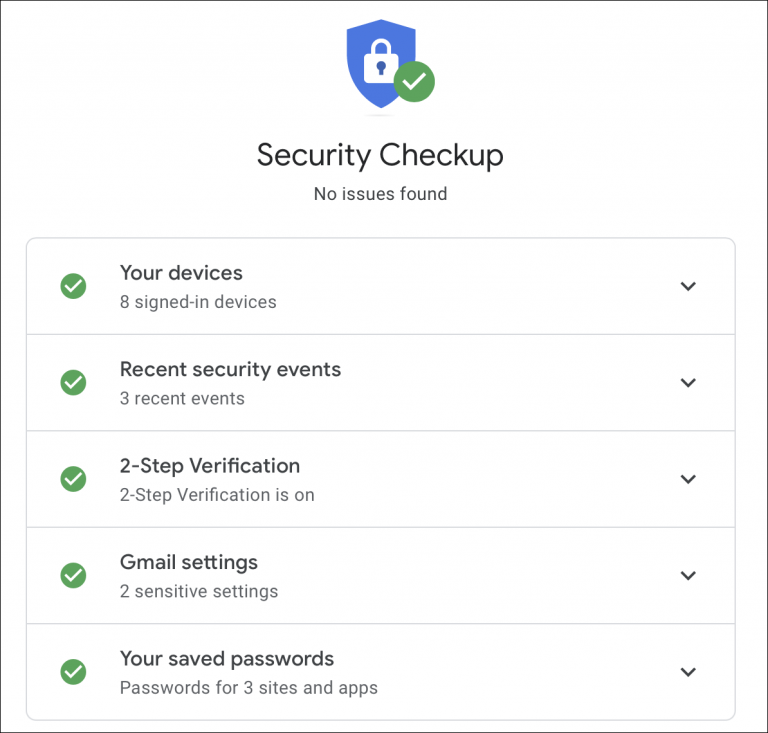
\includegraphics[width=0.75\linewidth]{images/google-security} 

}

\caption{Algunos de los ajustes que puedes hacer de seguridad en google.}\label{fig:unnamed-chunk-10}
\end{figure}

Además, recuerda que el resto de plataformas como Facebook, Linkedin, Instagram, X, Tiktok, etc. también ofrecen este tipo servicio para que puedas configurar tu seguridad y para sentirte más seguro.

\section{Contraseñas}\label{contraseuxf1as}

Una contraseña, clave o password es un mecanismo de autenticación que permite verificar tu identidad para acceder a un servicio, aplicación o dispositivo. Su seguridad depende de que únicamente tú conozcas esa información. \citep{WIKI-password}.

Cuando accedes a un servicio, este te solicita una contraseña. Si la contraseña introducida coincide con la registrada, se concede el acceso; en caso contrario, se deniega.

La contraseña sigue siendo uno de los métodos de autenticación más utilizados, pero también uno de los principales objetivos de los ciberdelincuentes. Por ello, es importante crear contraseñas que sean difíciles de adivinar o descubrir mediante ataques automatizados.

Cambio de paradigma en la creación de contraseñas (De las reglas antiguas a las recomendaciones modernas del NIST)

Durante muchos años se enseñó a crear contraseñas siguiendo reglas rígidas de:

\begin{itemize}
\item
  Debes incluir números.
\item
  Utiliza una combinación de letras mayúsculas y minúsculas.
\item
  Incluye caracteres especiales. Ejemplos: * ? ! @ \# \$ / () \{\} = . , ; :
\item
  Una longitud mayor o igual a 8 caracteres.
\item
  No debes incluir espacios en blanco.
\end{itemize}

Sin embargo, las guías modernas, especialmente el estándar NIST SP 800‑63B y su actualización SP 800‑63‑4, han demostrado que estas prácticas no aumentan la seguridad real y, en muchos casos, empeoran la experiencia del usuario.

A continuación se muestra cómo ha cambiado el enfoque:

Práctica antigua (obsoleta):

\begin{itemize}
\item
  Obligar a incluir números, símbolos y mayúsculas.
\item
  Prohibir espacios en blanco.
\item
  Usar trucos mnemotécnicos como M1C0ntr4s3ñ4!
\item
  Crear contraseñas cortas pero ``complejas''.
\item
  Cambiar la contraseña cada 30/60/90 días.
\end{itemize}

Problemas de este enfoque:

\begin{itemize}
\item
  Los usuarios crean patrones predecibles (Casa2024!, Gato123?).
\item
  Las transformaciones son fáciles de romper por herramientas automáticas.
\item
  Las contraseñas se vuelven difíciles de recordar y se reutilizan más.
\item
  La complejidad artificial no detiene ataques modernos.
\item
  Los cambios periódicos generan fatiga y contraseñas más débiles.
\end{itemize}

Práctica moderna (según NIST SP 800‑63B / SP 800‑63‑4):

\begin{itemize}
\item
  Priorizar la longitud sobre la complejidad.
\item
  Permitir y fomentar frases largas (passphrases).
\item
  Permitir espacios en blanco.
\item
  Evitar reglas de composición obligatoria.
\item
  Comprobar la contraseña contra listas de contraseñas filtradas o comunes.
\item
  Cambiar la contraseña solo si hay indicios de compromiso.
\end{itemize}

Ventajas del enfoque moderno:

\begin{itemize}
\item
  Las passphrases son más fáciles de recordar y mucho más difíciles de romper.
\item
  La longitud aporta más entropía que cualquier símbolo obligatorio.
\item
  Se reducen los patrones predecibles.
\item
  Se mejora la usabilidad sin sacrificar seguridad.
\item
  Se evita la fatiga del usuario y la reutilización de contraseñas.
\end{itemize}

Ejemplo comparativo:

Antes (obsoleto):

\begin{itemize}
\tightlist
\item
  M1Cu3nt4S3gur4!: Difícil de recordar, fácil de predecir, vulnerable a ataques offline.
\end{itemize}

Ahora (recomendado):

\begin{itemize}
\tightlist
\item
  mi perro duerme en mi sofá azul: Mucho más larga, más resistente y más fácil de recordar.
\end{itemize}

Fuente oficial: NIST (National Institute of Standards and Technology) de Estados Unidos, un organismo público que desarrolla estándares y guías técnicas ampliamente utilizados en todo el mundo. En ciberseguridad, NIST es una referencia clave porque publica las Digital Identity Guidelines, que establecen buenas prácticas modernas para contraseñas, autenticación y gestión de identidades. \citep{NIST}

Por otro lado, actualmente, muchos servicios ofrecen claves de acceso (passkeys), una alternativa más segura que las contraseñas tradicionales. Cuando estén disponibles, es recomendable utilizarlas.

Pero ¿En qué consisten las passkeys?

Las \href{https://www.eset.com/latam/blog/cultura-y-seguridad-digital/que-es-una-passkey-y-por-que-es-mejor-que-una-contrasena-tradicional/}{passkeys} son un método de autenticación moderno basado en criptografía de clave pública, que sustituye por completo a las contraseñas. En lugar de escribir una clave que puede ser robada, filtrada o adivinada, el dispositivo del usuario genera dos claves:

\begin{itemize}
\item
  Una clave pública, que se guarda en el servicio.
\item
  Una clave privada, que nunca sale del dispositivo.
\end{itemize}

Para iniciar sesión, el servicio envía un desafío que solo la clave privada puede firmar. El usuario se autentica con un gesto sencillo:

\begin{itemize}
\item
  Huella dactilar
\item
  Reconocimiento facial
\item
  PIN del dispositivo
\item
  Patrón de desbloqueo
\end{itemize}

La clave privada nunca se transmite, por lo que no puede ser robada en una filtración ni capturada por phishing.

Ventajas de las passkeys:

\begin{itemize}
\item
  Resistentes al phishing: no se pueden engañar con webs falsas.
\item
  No se pueden filtrar: no existe una contraseña que robar.
\item
  No requieren recordar nada.
\item
  No dependen de reglas de complejidad ni cambios periódicos.
\item
  Funcionan en varios dispositivos mediante sincronización segura.
\end{itemize}

A su vez también han de ser fáciles de recordar, pero debes de huir de patrones poco seguros y fáciles de adivinar. A continuación, algunos ejemplos de contraseñas que nunca debes utilizar:

\begin{itemize}
\item
  Qwerty
\item
  1234
\item
  Asdfg
\item
  Password
\item
  11111
\item
  Usar datos personales como la fecha de nacimiento, nombre mascota, etc.
\end{itemize}

En el siguiente enlace encontrarás una lista de las \href{https://nordpass.com/most-common-passwords-list/}{contraseñas más comunes} que jamás deberías utilizar. Échale un vistazo por si alguna de esas se parece a la tuya.

Otras recomendaciones que debes tener siempre presente:

\begin{itemize}
\item
  No compartas tus contraseñas con nadie.
\item
  No reutilices la misma contraseña en diferentes servicios.
\item
  Evita introducir tus contraseñas en dispositivos públicos o no confiables.
\item
  Puedes usar el gestor de contraseñas integrado en tu navegador, siempre que tu dispositivo esté protegido con PIN, biometría o contraseña. Los navegadores modernos cifran las contraseñas y son una opción segura para la mayoría de usuarios.
\item
  Usar Security keys o \href{https://es.digitaltrends.com/computadoras/las-mejores-llaves-de-seguridad-usb/}{llave de seguridad}. Verás que son más adelante en esta misma unidad en el apartado de MFA (Multi-Factor Authentication)
\item
  Usa la \href{https://www.bbva.es/finanzas-vistazo/ciberseguridad/seguridad-en-internet/verificacion-en-dos-pasos.html}{verificación en dos pasos} también conocida como autenticación doble y que verás en detalle más adelante en esta misma unidad.
\item
  Usa la \href{https://www.osi.es/es/actualidad/blog/2019/02/27/el-factor-de-autenticacion-doble-y-multiple}{autenticación de factor múltiple}, que también verás con más detalle en esta misma unidad.
\end{itemize}

La forma más segura y práctica de gestionar tus contraseñas es utilizar un gestor de contraseñas. Estos servicios generan claves robustas, las almacenan cifradas y te permiten usarlas sin tener que recordarlas todas. Además, reducen el riesgo de reutilizar contraseñas o de guardarlas en lugares inseguros.

Algunos gestores recomendados son:

\begin{itemize}
\item
  \href{https://bitwarden.com/}{Bitwarden}.
\item
  \href{https://keepassxc.org/}{KeePassXC}.
\item
  \href{https://www.lastpass.com/es/}{LastPass}.
\item
  \href{https://passwords.google.com/}{Google passwords}.
\item
  \href{https://nordpass.com/homepage/}{NordPass}.
\end{itemize}

Los gestores de contraseñas modernos cifran tus claves localmente y solo se desbloquean con tu biometría, PIN o contraseña maestra, por lo que son una opción segura para la mayoría de usuarios.

Puedes usar herramientas online para entender la robustez de una contraseña o passphrase, pero no introduzcas nunca tu contraseña real en estos sitios. Úsalos solo para probar ejemplos o variantes que no utilices en ningún servicio.

Algunos recursos útiles:

\begin{itemize}
\item
  \href{https://www.security.org/how-secure-is-my-password/}{How Secure Is My Password}: Estima el tiempo necesario para romper una contraseña mediante ataques offline.
\item
  \href{https://password.kaspersky.com/}{Password Check}: Analiza patrones débiles y longitud.
\item
  \href{https://www.ontek.net/test-contrasenas/}{Test contraseñas}: Mide la fortaleza aproximada de una clave.
\item
  \href{https://www.hivesystems.io/blog/are-your-passwords-in-the-green}{Hive Systems}: Muestra tablas actualizadas con tiempos estimados de crackeo según longitud y tipo de ataque.
\end{itemize}

Por otro lado si eres de las personas que te gusta tener todo bajo control puedes usar este servicio de Google llamado \href{https://www.blog.google/technology/safety-security/google-password-checkup-cross-account-protection/}{Password Checkout} o estos otros llamados \href{https://haveibeenpwned.com/Passwords}{Haveibeenpwned Passwords} para averiguar si alguna de tus contraseñas ha sido comprometida.

En un apartado como este donde se ha hablado de contraseñas desde sus diferentes ángulos no puede faltar entender cómo los ciberatacantes roban las contraseñas, aquí los 5 métodos más comunes:

\begin{itemize}
\item
  Phishing: Te engañan con correos o webs falsas para que introduzcas tu contraseña.
\item
  Filtraciones de datos: Contraseñas expuestas por brechas en servicios que luego se reutilizan en otros sitios.
\item
  Fuerza bruta: Prueban millones de combinaciones por segundo hasta acertar.
\item
  Keyloggers: Malware que registra lo que escribes en el teclado.
\item
  Ingeniería social: Manipulación psicológica para que reveles tu contraseña sin darte cuenta.
\end{itemize}

A modo de conclusión, y para terminar, si tuviésemos que simplificar todo lo anterior en tres principios esenciales para crear contraseñas seguras, serían los siguientes:

\begin{itemize}
\item
  Deben ser secretas: no deben compartirse con nadie bajo ninguna circunstancia.
\item
  Deben ser robustas: prioriza la longitud (idealmente 15 caracteres o más) y utiliza frases largas fáciles de recordar. No es necesario imponer reglas de complejidad (símbolos, números, mayúsculas), pero sí evitar patrones predecibles.
\item
  Deben ser únicas: usa una contraseña distinta para cada servicio. Nunca reutilices la misma clave en varias cuentas.
\end{itemize}

\section{Protocolo https}\label{protocolo-https}

El Protocolo Seguro de Transferencia de Hipertexto (en inglés, Hypertext Transfer Protocol Secure o HTTPS) es la versión segura del protocolo HTTP y se utiliza para proteger la comunicación entre el navegador y los sitios web \citep{WIKI-https}.

HTTPS emplea protocolos criptográficos TLS (Transport Layer Security) para crear una conexión cifrada entre el navegador y el servidor web. Gracias a este cifrado, la información intercambiada, como nombres de usuario, contraseñas, datos personales o información bancaria, viaja protegida frente a posibles interceptaciones por parte de terceros.

De este modo, aunque un atacante consiguiera interceptar la comunicación, únicamente obtendría datos cifrados que no podría interpretar ni modificar fácilmente.

Identificar si un sitio web utiliza HTTPS es muy sencillo. Basta con comprobar que la dirección web comienza por \texttt{https://}. Además, los navegadores modernos muestran información sobre la seguridad de la conexión al pulsar sobre el icono de información o seguridad situado junto a la dirección web. Al acceder a esta información, el navegador muestra detalles sobre la conexión segura, el certificado digital utilizado, las cookies almacenadas y otros aspectos relacionados con la configuración y seguridad del sitio web.

En este punto vamos a desmitificar la falsa sensación de confianza, que durante muchos años se ha divulgado en torno al candado en la barra de direcciones url del navegador. El candado hacía pensar que el contenido de la página era seguro. Lo cual no es cierto. Ya que los certificados de cifrado seguro los emiten terceros y los ciberestafadores pueden hacerse igualmente con uno. Sobre todo si se trata del certificado de dominio, que el único requisito es que la persona figure como contacto de administrador de dominio en el registro WHOIS de un nombre de dominio. Se trata del nivel más bajo de autenticación utilizado para validar certificados SSL.

Si quieres más información sobre los diferentes tipos de certificados lee el siguiente artículo \href{https://www.digicert.com/es/difference-between-dv-ov-and-ev-ssl-certificates}{¿Cuál es la Diferencia Entre los Certificados SSL DV, OV y EV?}

Además algunos navegadores eliminaron el icono del candado porque el protocolo HTTPS se ha convertido en el estándar predeterminado de internet, haciendo que un indicador de ``sitio seguro'' sea redundante \citep{CONFIDENCIAL-candado}.

En el enlace del Incibe \href{https://www.incibe.es/ciudadania/blog/que-hacer-si-el-navegador-nos-dice-que-estamos-intentando-acceder-un-sitio-no}{Qué hacer si el navegador nos dice que estamos intentando acceder a un sitio no seguro} explican el aviso del navegador cuando nos advierte que se trata de un sitio no seguro, o lo que es lo mismo, que cuando el navegador se está refiriendo a que el sitio web tiene un protocolo ``http: //'' sin la ``S'' en lugar de ``https: //'' con la ``S''.

\section{Compras y transacciones}\label{compras-y-transacciones}

Para comprar por Internet debes tomar cuantas más precauciones mejor para evitar cualquier tipo de fraude. Los factores a tener en cuenta son los siguientes:

\begin{itemize}
\item
  Evita sitios webs que no te inspiren confianza: Por ello solo debes compras a través de webs y aplicaciones oficiales.
\item
  Busca valoraciones y opiniones: Para ello dispones de las reseñas de Google maps, así como también de plataformas como \href{https://es.trustpilot.com/}{Trust Pilot}, \href{https://es.gowork.com/}{Gowork}, \href{https://esopiniones.com/}{Esopiniones}, \href{https://www.localguidesconnect.com/}{Local guides connect} o \href{https://www.tripadvisor.es/}{TripAdvisor}.
\item
  Utiliza plataformas que identifican webs fraudulentas como \href{https://fakeinet.com/}{Fakeinet}, \href{https://desenmascara.me/}{Desenmascarame} o \href{https://dnstwist.it/}{Dnstwist} que disponen de un listado de posibles tiendas falsas.
\item
  Usa plataformas que verifican si la web ha sido hackeada, como \href{https://www.scamadviser.com/}{Scamadviser} o \href{https://urlscan.io/}{Urlscan}.
\item
  Usa solo plataformas con protocolo HTTPS: Visto en el apartado anterior. Y recuerda que tener el candado no garantiza que la web sea legítima. Ya que los certificados de cifrado seguro los emiten terceros y los ciberestafadores pueden hacerse igualmente con uno.
\item
  Utiliza navegación privada: Así evitarás que se registre el historial de navegación.
\item
  Trata de usar pasarelas de pago: Evita en lo posible el uso de tarjetas de crédito y opta por una pasarela de pago, como puede ser \href{https://www.paypal.com/es/home}{PayPal}, te estarás garantizando la compra, además de disponer de protocolos de devolución del importe muy efectivos. Otra posibilidad es utilizar métodos de pago que incorporen protección al comprador, como tarjetas con sistemas de reclamación o servicios de pago intermediarios. Evita realizar transferencias directas, pagos mediante criptomonedas o sistemas de pago instantáneo cuando no conozcas plenamente al vendedor, ya que recuperar el dinero suele ser mucho más difícil.
\item
  En el caso de usar tarjeta de crédito usa siempre la misma o mejor aún utiliza tarjetas monedero o virtuales que facilitan los bancos con el fin de depositar solo en dinero con el que quieras hacer la compra y activa las notificaciones de operaciones de tu banco para detectar rápidamente cualquier cargo no autorizado.
\item
  Conserva los justificantes de compra, correos electrónicos y facturas hasta confirmar que has recibido el producto correctamente.
\item
  Haz comprobaciones adicionales:

  \begin{itemize}
  \item
    Comprueba desde cuándo existe el dominio de la página web. Muchas tiendas fraudulentas utilizan dominios registrados hace pocos días o semanas.
  \item
    Analiza la dirección web para detectar pequeñas modificaciones del nombre de una marca conocida (por ejemplo, letras cambiadas, caracteres especiales o dominios poco habituales).
  \item
    Comprueba que la web está adherida a alguna plataforma de confianza online, como, por ejemplo, \href{https://www.confianzaonline.es/}{Confianza Online}. Se trata del único sello de calidad que cuenta con los reconocimientos de la Comisión Europea, el Instituto Nacional de Consumo o la Agencia Española de Protección de datos, además de estar respaldado por el Ministerio de Industria, Energía y Turismo. Y acredita que se cumple con los estándares de privacidad y protección de datos de los usuarios entre otros. También existe el \href{https://www.aenor.com/certificacion/tecnologias-de-la-informacion/buenas-practicas-comercio-electronico}{Certificado de comercio electrónico} expedido por Aenor.
  \item
    Verifica que reciben análisis de seguridad periódicos realizados por plataformas como \href{https://www.mcafeesecure.com/certification}{McAfee Secure}.
  \item
    Asegúrate que disponen de certificados de autenticidad de la web y seguridad de las transacciones como los que ofrece \href{https://es.norton.com/internet-security}{Norton secured} o \href{https://www.comodo.com/home/internet-security/secure-shopping.php}{Comodo secure}.
  \item
    También existen plugins como \href{https://chrome.google.com/webstore/detail/historial-de-precios/fdeopiliemdomncemeibjpmccgmnkfig?hl=es-419&authuser=0}{Historial de precios} o \href{https://chrome.google.com/webstore/detail/alitools-shopping-assista/eenflijjbchafephdplkdmeenekabdfb?hl=es-419&authuser=0}{Alitools shopping assistan} que verifican si el precio del producto o servicio que deseas adquirir ha sido inflando por algún tipo de campaña publicitaria, como es el caso del Black Friday en los que suelen subir los precios para justificar su descuento.
  \item
    En primera instancia desconfía de los productos o servicios a precios muy inferiores al real o con suculentos descuentos.
  \item
    Verifica que las reseñas sean legítimas con plataformas como \href{https://www.ratebud.ai/}{Amazon Review Checker}. Si quieres saber más sobre las campañas de reseñas fraudulentas lee esta entrada sobre \href{https://www.genbeta.com/actualidad/asi-incentivaban-a-crear-resenas-falsas-proveedores-chinos-baneados-amazon}{reseñas falsas}.
  \item
    Los sellos y certificados los encontrarás normalmente en la parte inferior de la web en forma de logos y debes hacer click en ellos para obtener más información sobre la entidad que los expide y la vigencia de éstos, ya que muchas webs fraudulentas utilizan sellos falsos.
  \end{itemize}
\end{itemize}

\begin{figure}

{\centering \includegraphics[width=0.75\linewidth]{images/sellos-de-confianza-online} 

}

\caption{Sellos y certificados de comercio online.}\label{fig:unnamed-chunk-11}
\end{figure}

Tienes disponible más información sobre compras online en \href{https://www.aepd.es/sites/default/files/2019-09/guia-compra-segura-digital-web.pdf}{Compra segura en internet (Guía práctica)} y también dispones de esta entrada de \href{https://www.osi.es/es/actualidad/blog/2018/08/08/detectando-fraudes-analisis-de-una-web-de-venta-falsa}{cómo detectar fraudes y análisis de una web falsa}.

Por último ten siempre presente que, la inteligencia artificial ha facilitado la creación de tiendas fraudulentas con diseños muy profesionales, fotografías realistas, textos sin errores ortográficos e incluso asistentes virtuales capaces de responder automáticamente a tus preguntas. Por ello, no bases tu confianza únicamente en el aspecto visual de la página; verifica siempre la identidad del comercio mediante varios indicadores antes de realizar cualquier pago.

\section{Wi-Fi}\label{wi-fi}

Con respecto a la Wi-Fi nos encontramos ante dos escenarios: Wi-Fi propia y Wi-Fi ajena.

Uno de los peligros a los que más expuesto estás, es en el uso que haces de los puntos Wi-Fi ajenos. Ya que por lo general suelen ser puntos de accesos a la red gratuitos. En este escenario, existe el riesgo que aun tratándose de una red confiable puede haber sido hackeada por un tercero o que en primera instancia no provenga ni si quiera de una red de confianza. En cualquiera de los dos supuestos, tus dispositivos quedan expuestos y con ello, toda tu información sensible, a merced de ser espiado, robado o extorsionado.

Es por ello que debes tener la precaución de no hacer transacciones de ningún tipo, ni enviar datos sensibles. Es decir, usarla solo en caso de no te quede otra opción o en caso de tener que hacer cualquier búsqueda de carácter trivial.

Aun así, si usas una Wi-Fi pública estás expuesto entre otros ataques al conocido como Man-in-the-middle (Ataque de Intermediario en español), o el Packet sniffing. Si quieres más información al respecto visita el siguiente enlace \href{https://as.com/meristation/2020/02/04/betech/1580856719_548183.html}{Tipos de pirateo que puedes sufrir en un Wifi público}

Es de suponer que si estas en casa con Wi-Fi propia, estas recomendaciones no son tan necesarias. Pero sí, que sería muy recomendable por tu parte, que tuvieses muy en cuenta las recomendaciones que tienes a tu disposición en el apartado de Router en este manual. Además, es conveniente que si no has establecido las capas de seguridad que se recomiendan en ese apartado, hagas una revisión de tu conexión Wi-Fi, por si tienes algún intruso y de ser así poder eliminarlo. Para ello tienes a tu disposición en la web del Incibe un recurso llamado \href{https://www.osi.es/es/actualidad/blog/2019/09/25/descubre-y-elimina-los-intrusos-de-tu-red-wifi}{descubre y elimina a los intrusos de tu red wifi}.

Lo más recomendable es que siempre que puedas navegues con cable en lugar de Wi-Fi.

\section{Plugins o extensiones}\label{plugins-o-extensiones}

Las extensiones, también conocidas como extensiones o plugins, son pequeños programas que amplían las funcionalidades de una aplicación. En el caso de los navegadores web, permiten añadir nuevas características como bloquear publicidad, traducir páginas, gestionar contraseñas, comprobar la ortografía o mejorar la privacidad durante la navegación. Un ejemplo de estos es el archiconocido \href{https://getadblock.com/}{adBlock}, cuya función es la eliminar esos molestos anuncios de algunos portales webs.

Aunque resultan muy útiles, también pueden representar un riesgo para tu privacidad y seguridad. Muchas extensiones necesitan acceder al contenido de las páginas que visitas, por lo que una extensión maliciosa o comprometida podría recopilar información sobre tu actividad, modificar el contenido de las páginas web o mostrar publicidad no deseada.

Para reducir estos riesgos sigue estas recomendaciones:

\begin{itemize}
\item
  Instala únicamente las extensiones que realmente necesites. Cuantas menos tengas instaladas, menor será la superficie de exposición de tu navegador.
\item
  Descarga las extensiones únicamente desde el repositorio oficial de tu navegador. Aunque estos repositorios realizan controles de seguridad, ninguna revisión garantiza por completo que una extensión sea segura.
\item
  Comprueba quién es el desarrollador de la extensión, el número de instalaciones, las valoraciones de otros usuarios y la fecha de la última actualización. Una extensión abandonada o que lleva mucho tiempo sin actualizarse puede presentar vulnerabilidades.
\item
  Revisa los permisos que solicita antes de instalarla. Desconfía si una extensión solicita acceso a información que no necesita para realizar su función. Por ejemplo, una extensión para cambiar el aspecto del navegador difícilmente necesitará acceder a todas las páginas que visitas.
\item
  Mantén activadas las actualizaciones automáticas para recibir las correcciones de seguridad publicadas por sus desarrolladores.
\end{itemize}

Revisa periódicamente las extensiones instaladas y elimina aquellas que ya no utilices.

Actualmente, la inteligencia artificial también está siendo utilizada por los ciberdelincuentes para crear extensiones fraudulentas con descripciones muy convincentes, generar reseñas falsas o copiar la apariencia de extensiones legítimas. Por ello, no bases tu confianza únicamente en las valoraciones o en el aspecto profesional de la página de descarga; verifica siempre el desarrollador y los permisos que solicita la extensión.

Algunos ejemplos de extensiones ampliamente utilizadas son los bloqueadores de publicidad, los gestores de contraseñas, los traductores automáticos, los correctores ortográficos o las herramientas para comprobar el historial de precios durante las compras por Internet. Instálalas siempre desde las tiendas oficiales de tu navegador y únicamente cuando procedan de desarrolladores de confianza.

\begin{figure}

{\centering \includegraphics[width=0.75\linewidth]{images/plugin-navegador} 

}

\caption{Plugin traductor de Google seguido de otros plugin con diferentes funcionalidades.}\label{fig:unnamed-chunk-12}
\end{figure}

Si quieres ampliar tus conocimientos sobre las extensiones o plugins de los navegadores, puedes consultar la web de Incibe y su publicación \href{https://www.osi.es/es/actualidad/blog/2019/11/20/extensiones-superpoderes-para-los-navegadores}{extensiones: Superpoderes para los navegadores}.

\section{Descarga segura de aplicaciones y programas}\label{descarga-segura-de-aplicaciones-y-programas}

Siempre que necesites instalar una aplicación o un programa, descárgalo desde la página web oficial del desarrollador o desde la tienda oficial de tu sistema operativo (como Microsoft Store, App Store o Google Play, según el dispositivo que utilices). Evita descargar software desde páginas de terceros, ya que pueden distribuir versiones modificadas, desactualizadas o que incorporen programas no deseados e incluso código malicioso.

Aunque los antivirus constituyen una importante capa de protección, no son capaces de detectar todas las amenazas. Los ciberdelincuentes desarrollan continuamente nuevas técnicas para evitar su detección, por lo que no debes confiar únicamente en que un antivirus identificará cualquier archivo malicioso.

Algunos portales de descarga ofrecen programas muy populares, pero sustituyen el instalador original por otro propio que puede incluir publicidad, software no deseado o aplicaciones adicionales que se instalan si no prestas atención durante el proceso.

Presta especial atención a los archivos ejecutables, como los que tienen extensión .exe en Windows, ya que son los encargados de instalar o ejecutar programas. Aunque la mayoría son completamente legítimos, también son el formato más utilizado para distribuir malware \citep{RZ-exe}. Antes de ejecutarlos:

\begin{itemize}
\item
  Comprueba que proceden de una fuente oficial.
\item
  Verifica que el nombre del archivo coincide con el programa que deseas instalar.
\item
  Analiza el archivo con tu solución de seguridad si tienes cualquier duda.
\item
  Desconfía si el archivo te llega por correo electrónico, mensajería instantánea o redes sociales sin haberlo solicitado previamente.
\end{itemize}

También debes prestar atención durante el proceso de instalación. Lee cada pantalla del asistente y rechaza la instalación de programas adicionales, cambios en el navegador.

La inteligencia artificial también está siendo utilizada para crear páginas de descarga falsas prácticamente idénticas a las originales, generar campañas de phishing que suplantan a los desarrolladores de software o distribuir instaladores acompañados de instrucciones muy convincentes. Antes de descargar cualquier programa, comprueba que la dirección web corresponde realmente al sitio oficial y no te fíes únicamente del aspecto profesional de la página o de los resultados patrocinados de los buscadores.

Como norma general, si tienes dudas sobre el origen de un programa, es preferible no instalarlo hasta haber verificado su autenticidad. Unos minutos de comprobación pueden evitar la instalación de malware y la pérdida de información personal.

\section{Cierre de sesiones y uso de dispositivos ajenos}\label{cierre-de-sesiones-y-uso-de-dispositivos-ajenos}

Cuando utilizas cualquier servicio en internet, como tu correo electrónico, redes sociales o plataformas bancarias, el primer paso para proteger tu información es iniciar sesión con tus credenciales.

Si estás utilizando tu propio móvil u ordenador, mantener la sesión iniciada es cómodo y seguro, siempre y cuando tu dispositivo esté protegido con un PIN, contraseña o huella dactilar. Sin embargo, la regla cambia por completo si utilizas un dispositivo ajeno o público (como el de un amigo, una oficina o una biblioteca). En estos casos, si olvidas cerrar la sesión, tus datos personales, mensajes y cuentas quedarán totalmente expuestos a la siguiente persona que use ese equipo.

Para evitar riesgos innecesarios, adopta estos dos hábitos esenciales de seguridad moderna:

\begin{itemize}
\item
  Usa siempre el Modo Incógnito: Cuando vayas a iniciar sesión en un dispositivo que no es tuyo, abre una ventana de navegación privada. La gran ventaja es que, en cuanto cierras esa ventana, el navegador destruye automáticamente tus contraseñas, cookies e historial, impidiendo que nadie pueda entrar a tus cuentas.
\item
  Cierra sesión de forma remota si te despistas: Si te vas de un lugar y te asalta la duda de si dejaste tu cuenta abierta, no entres en pánico. Hoy en día, plataformas como Google, Microsoft o Meta (Facebook/Instagram) incluyen una sección de seguridad llamada ``Dispositivos activos'' o ``Dónde has iniciado sesión'' en los ajustes de tu cuenta. Desde allí, puedes pulsar un botón desde tu propio móvil para cerrar la sesión a distancia en cualquier otro equipo al instante.
\end{itemize}

Recuerda: Tu privacidad digital depende de dónde dejas tus llaves. No dejes nunca tus cuentas abiertas en territorio desconocido.

\section{2SV (Two Step Verification) o Verificación en Dos Pasos}\label{sv-two-step-verification-o-verificaciuxf3n-en-dos-pasos}

La mayoría de cuentas a día de hoy están configuradas para soportar lo que se conoce como SFA (Single Factor Authetication) o Factor de autenticación Simple, tamibén conocido como autenticación de un solo factor. Se trata del acceso a cuentas o servicios con el solo uso del usuario y una contraseña, algo que todo el mundo viene haciendo desde hace tiempo. Esto se ha vuelto en gran medida un gran riesgo, ya que si un tercero consigue hacerse con tu contraseña no tendrá ninguna dificultad para tomar el control.

Es por este motivo que cada vez más servicios están implementando lo que se conoce como 2SV (Two Step Verification) o Verificación en Dos Pasos. Este sistema funciona de la siguiente manera, justo después de introducir tu contraseña, se te envía una notificación de forma segura al dispositivo en el que hayas iniciado sesión, de manera que solo tienes que aprobar la notificación para realizar el inicio sesión. Algunos servicios como la \href{https://support.google.com/accounts/answer/185839?co=GENIE.Platform\%3DDesktop&hl=es}{verificación en dos pasos de Google} viene de manera nativa y tan solo tienes que activarla.

Como puedes ver, los dos pasos son:

\begin{enumerate}
\def\labelenumi{\arabic{enumi}.}
\tightlist
\item
  Usuario y contraseña: Que solo tú conoces.
\item
  Notificación: Recibes un aviso en tu dispositivo.
\end{enumerate}

\begin{figure}

{\centering \includegraphics[width=0.75\linewidth]{images/verificación-dos-pasos} 

}

\caption{Verificación en dos pasos.}\label{fig:unnamed-chunk-13}
\end{figure}

Según la fuente que uses para informarte puede ser que termines sin comprenderlo del todo, ya que algunos medios también entienden la verificación en dos pasos (2SV) como un 2FA (segundo factor de autenticación). La diferencia es tan sutil que a veces es difícil de discernir, pero podría entenderse si ves el 2SV como una notificación que recibes y que apruebas sin más y la 2FA como un código que has de introducir. No obstante si quieres más información, en este enlace sobre \href{https://www.osi.es/es/actualidad/blog/2017/01/17/verificacion-en-dos-pasos-que-es-y-como-me-puede-ayudar}{verificación en dos pasos} encontrarás más detalles, además de enlaces hacia las distintas plataformas y redes sociales más populares para que puedas implementarlo.

Es extremadamente recomendable que uses este sistema de verificación en la medida que puedas. Recuerda que de un modo u otro la mayoría de servicios y plataformas disponen de esta capa de seguridad. Normalmente las encontrarás en Ajustes y Seguridad.

\section{MFA (Multi-Factor Authentication) o Autenticación de Factores Múltiples}\label{mfa-multi-factor-authentication-o-autenticaciuxf3n-de-factores-muxfaltiples}

La autenticación de factor múltiple es una forma eficaz de aumentar la protección de las cuentas de usuario contra las amenazas más comunes, como los ataques de phishing, apropiación de cuentas, etc. Y se trata un método de control de acceso informático, en el que a un usuario, se le concede acceso al sistema solo después de que presente dos o más pruebas o factores diferentes de que es quien dice ser. Estas pruebas pueden ser diversas, como una contraseña, clave secundaria rotativa, un certificado digital instalado en el equipo, un token físico, etc. entre otros y son éstos lo que se conocen como factores de autenticación \citep{WIKI-multiple-factor}.

Son tres los tipos de factores de autenticación:

\begin{itemize}
\item
  Algo que sabes: Factor de conocimiento (contraseña, respuesta a una pregunta, un PIN).
\item
  Algo que tienes: Factor de posesión (tarjeta, smartphone, token hardware como las Security keys).
\item
  Algo que eres: Factor biométrico (huellas dactilares, escaneos de retina, reconocimiento facial, reconocimiento de voz o el comportamiento de un usuario).
\end{itemize}

Uno de los ejemplos de autenticación en dos factores más común es la acción que realizas cuando vas a sacar dinero de un cajero. Por un lado, metes la tarjeta (algo que tienes) y luego pones el PIN (algo que sabes). Esto es lo que se conoce como la autenticación en dos pasos o 2FA (segundo factor de autenticación), que es uno de los tipos más comunes de MFA y que a veces tiende a confundirse con la verificación en dos pasos 2SV (Two Step Verification) que puedes verla en esta misma unidad.

Otro ejemplo son los inicios de sesión en los que se necesita un código adicional que es gestionado a través de correo electrónico, SMS o llamadas telefónicas, como es el caso de algunas entidades bancarias, esto es lo que se conoce como OTP por sus siglas en inglés ``One-Time Password'' y en castellano ``contraseña de uso único''. Y en otros supuestos, aunque la plataforma disponga de dicho servicio necesitarás una aplicación externa como \href{https://support.google.com/accounts/answer/1066447?co=GENIE.Platform\%3DAndroid&hl=es-419}{Google Authenticator} o \href{https://www.microsoft.com/es-es/account/authenticator}{Microsoft authenticator} entre otras y que se trata de una App de autenticación en dos pasos, que te genera el código adicional, que ha de ser utilizado inmediatamente ya que éste expira con el tiemplo.

También puedes hacer uso de autenticación de factores múltiples con lo que se conoce como Security Key o llave de seguridad. Se trata de un dispositivo hardware generalmente con conexión USB y necesitarás usar como segundo factor de autenticación una vez hayas introducido tu usuario y contraseña. En la publicación \href{https://es.digitaltrends.com/computadoras/las-mejores-llaves-de-seguridad-usb/}{las mejores llaves de seguridad usb} encontrarás algunos de los más utilizados y recuerda siempre comprar en las plataformas oficiales o de confianza.

\begin{figure}

{\centering \includegraphics[width=0.5\linewidth]{images/autenticación-factor-múltiple} 

}

\caption{Autenticación de factores múltiples.}\label{fig:unnamed-chunk-14}
\end{figure}

En la mayoría de los casos solo se combinan dos de estos tres factores, aunque existe la posibilidad de implementar los tres si se viene necesario. Más información en \href{https://www.santander.com/es/stories/pon-una-capa-extra-de-seguridad-online-con-la-autenticacion-multifactor}{Banco Santander stories} y \href{https://protegermipc.net/2016/03/18/autenticacion-en-dos-factores-vs-autenticacion-en-dos-pasos/}{Autenticación en dos factores vs autenticación en dos pasos}.

\section{AntiBotnet}\label{antibotnet}

Una botnet es una red de dispositivos infectados con un programa malicioso (malware) que permite a un ciberdelincuente controlarlos de forma remota sin que sus propietarios sean conscientes de ello. Cada uno de estos dispositivos se conoce como ``bot'' o ``equipo zombi''.No existe un número mínimo de equipos para crear un botnet. Los botnets pequeños pueden incluir cientos de PCs infectados, mientras que los mayores utilizan millones de equipos \citep{INCI-botnet}.

Aunque tradicionalmente las botnets estaban formadas principalmente por ordenadores personales, hoy también pueden incluir teléfonos móviles, routers domésticos, cámaras de videovigilancia, dispositivos inteligentes del hogar (IoT) y otros equipos conectados a Internet.

Los ciberdelincuentes utilizan estas redes para realizar diferentes actividades maliciosas, como enviar grandes cantidades de correo no deseado, lanzar ataques de denegación de servicio (DDoS), distribuir malware, ocultar el origen de otros ataques o utilizar los recursos de los dispositivos infectados sin autorización.

En muchos casos, una infección puede pasar desapercibida. No obstante, algunos indicios pueden ser un funcionamiento más lento del dispositivo, un consumo inusual de la conexión a Internet o un aumento de la actividad del equipo sin que estés utilizándolo.

Para reducir el riesgo de que tus dispositivos formen parte de una botnet:

\begin{itemize}
\item
  Mantén actualizado el sistema operativo y todas las aplicaciones.
\item
  Actualiza periódicamente el firmware del router y de los dispositivos inteligentes.
\item
  Cambia las contraseñas predeterminadas de los dispositivos conectados.
\item
  Descarga aplicaciones únicamente desde fuentes oficiales.
\item
  Utiliza un antivirus y mantén activada la protección frente a malware.
\end{itemize}

La inteligencia artificial está facilitando la automatización de campañas de phishing y otras técnicas empleadas para distribuir malware. Por ello, resulta aún más importante desconfiar de mensajes inesperados y mantener los dispositivos correctamente protegidos y actualizados.

Si sospechas que alguno de tus dispositivos puede estar comprometido, puedes utilizar el \href{https://www.incibe.es/ciudadania/herramientas/servicio-antibotnet/}{servicios antibotnet} que identifican si desde tu conexión a internet se ha detectado algún incidente de seguridad relacionado u otras amenazas. Además en el siguiente enlace obtendrás una suite de rastreo y eliminación de Botnet \href{https://www.incibe.es/ciudadania/servicio-antibotnet/cleaners}{Servicio Antibotnet: Cleaners}.

\section{Bluetooth}\label{bluetooth}

Bluetooth es una tecnología de comunicación inalámbrica que permite conectar dispositivos cercanos, como auriculares, relojes inteligentes, teclados, altavoces o sistemas de manos libres del automóvil, etc. \citep{IONOS-bluetooh}.

Las versiones actuales de Bluetooth incorporan mecanismos de seguridad mucho más robustos que los de hace años. No obstante, como cualquier tecnología inalámbrica, pueden aparecer vulnerabilidades que sean aprovechadas por ciberdelincuentes, especialmente si el dispositivo no está actualizado.

Entre los ataques más conocidos se encuentran:

\begin{itemize}
\item
  Bluejacking: envío de mensajes o contenido no solicitado a dispositivos cercanos.
\item
  Bluesnarfing: acceso no autorizado a información del dispositivo aprovechando vulnerabilidades.
\item
  Bluebugging: explotación de fallos de seguridad para obtener un cierto control sobre el dispositivo.
\end{itemize}

Aunque estos ataques son mucho menos frecuentes en dispositivos modernos correctamente actualizados, siguen siendo un ejemplo de los riesgos que pueden existir cuando el software presenta vulnerabilidades.

Además de estas técnicas de ataque, a lo largo de los años se han descubierto diversas vulnerabilidades en el propio protocolo Bluetooth y en su implementación en distintos sistemas operativos y dispositivos. Algunas de las más conocidas han recibido nombres como BlueBorne, KNOB, BIAS, BrakTooth o BLUFFS. Estos fallos de seguridad pueden permitir, en determinadas circunstancias, el acceso no autorizado al dispositivo, la interceptación de comunicaciones o la degradación de los mecanismos de protección. Por ello, resulta fundamental mantener siempre actualizado el sistema operativo y el firmware de los dispositivos que utilizan esta tecnología.

Para utilizar Bluetooth de forma segura:

\begin{itemize}
\item
  Mantén actualizado el sistema operativo y el firmware de tus dispositivos.
\item
  Empareja únicamente dispositivos de confianza.
\item
  Comprueba siempre el código de emparejamiento cuando se muestre en ambos dispositivos.
\item
  Desactiva el modo visible o detectable cuando no sea necesario.
\item
  Elimina de la lista los dispositivos que ya no utilices.
\item
  Si no vas a utilizar Bluetooth durante un tiempo, especialmente en lugares públicos, puedes desactivarlo para reducir la superficie de exposición.
\end{itemize}

Recuerda que la mayoría de los ataques mediante Bluetooth requieren que el atacante se encuentre relativamente cerca del dispositivo, por lo que el riesgo suele ser menor que el de amenazas que actúan a través de Internet.

El riesgo que corres cuando tienes este servicio activado es que el dispositivo de un tercero acabe sincronizándose con el tuyo, con los riesgos expuestos.
Si quieres más información visita el siguiente enlace \href{https://computerhoy.com/noticias/tecnologia/diferencias-principales-ataques-bluetooth-bluesnarfing-bluejacking-bluebugging-1087867}{Diferencias entre los principales ataques por bluetooth: Bluesnarfing, Bluejacking y Bluebugging}.

\section{NFC (Near field communication)}\label{nfc-near-field-communication}

NFC (Near Field Communication) es una tecnología inalámbrica de muy corto alcance que permite intercambiar información entre dispositivos cercanos. Se utiliza habitualmente para realizar pagos sin contacto, identificarte mediante tarjetas o teléfonos móviles, acceder a edificios, validar billetes de transporte o leer etiquetas inteligentes \citep{IONOS-nfc}.

Su reducido alcance, de apenas unos centímetros, constituye una de sus principales medidas de seguridad, ya que requiere que los dispositivos se encuentren muy próximos para poder comunicarse.

Aunque NFC es una tecnología segura cuando se utiliza correctamente, existen algunos riesgos que conviene conocer:

\begin{itemize}
\item
  Ejecución de programas maliciosos: ejecuta código en terminales Android simplemente acercando una etiqueta NFC al dispositivo.
\item
  Pagos sin autorización: realiza compras por proximidad sin consentimiento.
\item
  Transmisión de datos sin cifrar: lee datos como el nombre, apellidos, el número de la tarjeta y, en algunos casos, las transacciones realizadas.
\item
  Copia de datos bancarios: con el empleo de Lectores con comunicación inalámbrica NFC.
\end{itemize}

Los sistemas actuales de pago mediante NFC incorporan mecanismos criptográficos y otras medidas de seguridad que dificultan considerablemente la copia de los datos bancarios. No obstante, cuando se trata de ciberseguridad, conviene mantener siempre una actitud prudente y seguir las recomendaciones de seguridad.

No obstante, debemos tener siempre presente que algunos ciberdelincuentes también utilizan técnicas de ingeniería social para convencerte de acercar tu teléfono a etiquetas NFC manipuladas o de instalar aplicaciones maliciosas tras leerlas. Antes de interactuar con una etiqueta NFC, asegúrate de que procede de una fuente de confianza.

Para utilizar NFC de forma segura:

\begin{itemize}
\item
  Mantén actualizado el sistema operativo de tu dispositivo.
\item
  Activa NFC únicamente cuando vayas a utilizarlo, si no lo necesitas de forma habitual.
\item
  No acerques tu dispositivo a etiquetas NFC de origen desconocido.
\item
  Revisa periódicamente los movimientos de tus tarjetas y cuentas bancarias.
\item
  Protege tu dispositivo mediante un método de desbloqueo seguro.
\end{itemize}

Si utilizas tarjetas con pago sin contacto y te preocupa una posible lectura accidental, puedes emplear fundas con protección RFID/NFC. No obstante, para la mayoría de las personas, el riesgo es reducido y mantener la tarjeta bajo tu control sigue siendo la medida de protección más importante.

\chapter{Amenazas}\label{amenazas}

\section{Principales amenazas}\label{principales-amenazas}

En lo referente a la seguridad de tus dispositivos debes tener en cuenta la diversidad de amenazas que existen, tales como virus, spywares, troyanos, gusanos y que pueden comprometer tus dispositivos y toda la información que en ellos contengas.

La mayoría de éstos están catalogado como Malware. Un Malware es un tipo de software malicioso con un primer objetivo inicial de infiltrarse en un equipo o sistema informático sin el consentimiento del usuario, para posteriormente actuar sobre él \citep{WIKI-malware}.

En este punto es importante que sepas cuáles son todas y cada una de las amenazas a las que estas expuesto, si no tienes las herramientas y no adoptas una actitud prudente en el uso de los dispositivos y la red.

En unidades anteriores viste que precauciones y herramientas debes adoptar para no correr riesgos. En esta unidad verás cuáles son estas amenazas y como llegan a tus dispositivos.

Las amenazas vienen de la mano de perfiles a los que conoces como hacker, ciberdelicuente, pirata informático, etc. Pero cabe destacar que estos conceptos no son lo mismo \citep{OSPI-ciberseguridad-espana}. Por lo tanto:

\begin{itemize}
\item
  Ciberdelincuentes: Sus ataques se dirigen a objetivos concretos como escuelas, hospitales, instituciones, grandes empresas o bancos, entre muchos otros.
\item
  Ciberterroristas y ciberyihadistas: Organizaciones terroristas que han desarrollado sus propias divisiones informáticas, aunque todavía no parecen ser capaces de desarrollar ciberataques sofisticados.
\item
  Hackivistas: Grupos reivindicativos que actúan por razones ideológicas.
\item
  Cibervándalos: Simplemente responden al deseo de armar revuelo y suelen ser ciberdelincuentes amateurs y poco cualificados.
\end{itemize}

Dispones de más información en \href{https://www.incibe.es/aprendeciberseguridad/hacker-vs-ciberdelincuente}{hacker vs ciberdelincuente} y \href{https://www.osi.es/es/campanas/los-ciberdelincuentes-quienes-son/quienes-son-los-ciberdelincuentes-y-que-buscan}{¿Quiénes son los ciberdelincuentes y qué buscan?}.

\textbf{¿Cómo detectar si estás infectado?}

\begin{itemize}
\item
  Cambios en el navegador, página de inicio distinta, nuevos favoritos o barras de herramientas.
\item
  Ordenador ralentizado.
\item
  Ventanas emergentes inesperadas.
\item
  Perdida de espacio en la memoria ram o disco duro.
\item
  Apagón del equipo de manera inesperada.
\item
  Mensajes anormales a la hora de encender el equipo.
\item
  Mensajes de alertas inesperados.
\item
  Ficheros cambiados de nombre o desaparecidos.
\end{itemize}

\textbf{Una buena práctica para minimizar los riesgos es disponer de una suite de seguridad que estaría básicamente formada por:}

\begin{itemize}
\item
  Antivirus.
\item
  Anti-Spyware.
\item
  Firewall o corta fuegos.
\item
  Copia de seguridad.
\item
  Discos de arranque.
\item
  Anti-phishing. El phishing lo verás en esta misma unidad más adelante.
\end{itemize}

\textbf{Si hay menores en casa:}

\begin{itemize}
\item
  Control parental.
\item
  Filtro web que restringe el acceso a contenidos no apto para menores.
\end{itemize}

\textbf{Los tres ciberataques que encabezan el ranking son:}

\begin{enumerate}
\def\labelenumi{\arabic{enumi}.}
\item
  Fraude de ventas.
\item
  Vulnerabilidad de los equipos.
\item
  Infecciones por malware que pretenden borrar datos, alterar las funciones básicas del equipo, espiar y/o robar datos.
\end{enumerate}

\section{Virus}\label{virus}

Un virus es un programa informático diseñado para infectar archivos u ocasionar efectos molestos, destructivos e incluso irreparables en tu ordenador, dañando hardware, software y archivos \citep{PANDA-virus}.

Los virus tienen diferentes vías de entrada a tus equipos, como por ejemplo:

\begin{itemize}
\item
  Utilización de una memoria USB previamente infectada.
\item
  Descarga de contenidos mediante redes de compartición P2P, u otras fuentes poco fiables.
\item
  Apertura de algún fichero adjunto en un correo electrónico.
\item
  Visitar una web maliciosa o pulsar sobre alguna dirección acortada que se publican en redes sociales u otros medidos y que en realidad no sabes a qué páginas web te puede llevar.
\end{itemize}

\section{Gusanos informáticos}\label{gusanos-informuxe1ticos}

Los gusanos son en realidad una subclase de virus, por lo que comparten características similares \citep{PANDA-gusano}.

El principal objetivo de los gusanos es propagarse y afectar al mayor número de dispositivos posible, colapsar los ordenadores y las redes informáticas e impidiendo así el trabajo a los usuarios.

A diferencia de un virus, un gusano no necesita realizar cambios en los archivos de programas, sino que se aloja en diferentes ubicaciones del ordenador, principalmente la memoria RAM, para seguidamente clonarse a sí mismo y usar tus contactos y otros recursos del dispositivo para auto enviarse, a través del correo electrónico o programas P2P entre otros. Por lo que tienen la capacidad de propagarse sin la ayuda de una persona.

Los gusanos tienen diferentes vías de entrada a los equipos, como, por ejemplo:

\begin{itemize}
\item
  Utilización de una memoria USB previamente infectada.
\item
  Descarga de contenidos mediante redes de compartición P2P u otras fuentes poco fiables.
\item
  Apertura de algún fichero adjunto en un correo electrónico.
\item
  Visitar una web maliciosa o pulsar sobre alguna dirección acortada que se publican en redes sociales u otros medidos y que en realidad no sabes a qué páginas web te puede llevar.
\end{itemize}

\section{Troyanos}\label{troyanos}

Un Troyano o también llamado Caballo de Troya es una clase de malware que normalmente se camufla como software legítimo. Los ciberladrones utilizan este software malicioso para acceder en tus equipos y una vez dentro campar a sus anchas \citep{KASPER-troyano}.

Uno de los más peligrosos son los keylogger es un tipo de software o un dispositivo hardware específico que se encarga de registrar las pulsaciones que realizas a través de tu teclado. Posteriormente son guardadas en un fichero y remitido a través de la red a los ciberdelincuentes.

Pudiendo llegar también como virus o gusanos, una vez activados, los troyanos pueden permitir a los cibercriminales espiarte, robar tus datos confidenciales y obtener acceso por una puerta trasera a tu sistema.

Los métodos más comunes de infección de un troyano suelen ser:

\begin{itemize}
\item
  La descarga de programas piratas o \href{https://es.wikipedia.org/wiki/Cracking_(software)}{crackeados}.
\item
  Descarga de programas gratuitos desconocidos (juegos, salvapantallas y aplicaciones sencillas relacionadas con el entretenimiento).
\item
  Abrir archivos adjuntos infectados.
\item
  Abrir una imagen o cualquier otro tipo de archivo que sea en realidad un ejecutable con extensión modificada.
\item
  Visitar sitios web trampa, es decir, sitios en los que para poder ver los vídeos sea necesario descargar un códec que en realidad es el troyano.
\item
  Visitar una web maliciosa o pulsar sobre alguna dirección acortada que se publican en redes sociales u otros medidos y que en realidad no sabes a qué páginas web te puede llevar.
\item
  Descarga de contenidos mediante redes de compartición P2P u otras fuentes poco fiables.
\end{itemize}

Algunos de los troyanos con más incidencias son el \href{https://www.welivesecurity.com/la-es/2021/12/29/que-es-dropper-cual-es-funcion-esta-amenaza/}{Dropper} o los que usan \href{https://blogs.protegerse.com/2023/04/20/cuidado-con-las-falsas-facturas-varias-familias-de-troyanos-usan-archivos-pdf-para-propagarse/}{archivos PDF} para propagarse, pero recuerda que no son los únicos y que siempre están en constante evolución.

Existen herramientas que analizan y limpian los troyanos que se esconden en tu dispositivo y a su vez previene futuros ataques troyanos. Una de estas herramientas es el \href{https://www.avast.com/c-trojan-remover-tool}{Trojan remover}.

\section{Ransomware o programa rescate}\label{ransomware-o-programa-rescate}

El Programa rescate o ransomware, está dentro del conjunto de software malicioso que también se conoce como malware y que impiden utilizar el equipo mientras el usuario no pague una cierta cantidad de dinero. El virus bloquea o cifra la información o datos del equipo \citep{WIKI-ransomware}.

Para intimidar y engañar a las víctimas les hacen creer que han incurrido en algún tipo de actividad delictiva, como incitación al odio, terrorismo o pederastia, entre otros.

En la actualidad estos son unos de los ataques más virulentos. Según un estudio realizado por la compañía \href{https://www.pandasecurity.com/es/mediacenter/seguridad/2019-tsunami-del-ransomware/}{Panda Security} en el 2019 este delitito tuvo un incremento con respecto al año 2018 del 500\%. Y según un estudio del \href{https://www.ospi.es/es/}{Observatorio del Sector Público de Inetum} solo en 2018, el número de afectados por estos ataques fue de más de 1.000 millones en todo el planeta.

\begin{figure}

{\centering \includegraphics[width=0.75\linewidth]{images/ransomware} 

}

\caption{Ransomware (Malware).}\label{fig:unnamed-chunk-15}
\end{figure}

Las diferentes vías de entrada de ransomware a tu equipo son:

\begin{itemize}
\item
  Utilización de una memoria USB previamente infectada.
\item
  Descarga de contenidos mediante redes de compartición P2P, u otras fuentes poco fiables.
\item
  Apertura de algún fichero adjunto en un correo electrónico.
\item
  Visitar una web maliciosa o pulsar sobre alguna dirección acortada que se publican en redes sociales u otros medidos y que en realidad no sabes a qué páginas web te puede llevar.
\end{itemize}

En este punto cabe destacar que hay firmas de antivirus como AVG que pone a disposición del usuario una suite de herramientas gratuitas para \href{https://www.avg.com/es-es/ransomware-decryption-tools}{deshacer el cifrado del ransomware}, de igual modo tienes a tu disposición los \href{https://noransom.kaspersky.com/es/}{Descifradores de Ransomware Gratuitos} de Kaspersky y la oficina de seguridad del internauta también pone a disposición otros recursos para combatir el ransomware en el siguiente artículo \href{https://www.osi.es/es/actualidad/blog/2022/11/17/no-pagues-ningun-rescate-si-un-ransomware-ha-cifrado-tu-informacion}{¡No pagues ningún rescate si un ransomware ha cifrado tu información!}.

Además, en el caso del sistema operativo de Windows 10 en su última versión dispone de una protección de forma nativa contra ransomware, aunque esto no te garantiza estar inmunizado.

Algunos de los ransomware más mediáticos son \href{https://es.wikipedia.org/wiki/CryptoLocker}{CryptoLocker}, \href{https://es.wikipedia.org/wiki/Ransomware\#CryptoWall}{CryptoWall} y \href{https://es.wikipedia.org/wiki/WannaCry}{WannaCry}, pero no son los únicos, además de estar siempre en constante evolución y lo que es peor aún, éstos últimos irán dejando paso a otros mucho más nuevos y peligrosos.

\section{Spyware o software espía}\label{spyware-o-software-espuxeda}

El spyware es otro tipo de malware que se mantiene oculto mientras recopila información en secreto, que después transmite a una entidad externa, sin el conocimiento o el consentimiento del propietario del dispositivo \citep{AVAST-spyware}.

Puede supervisar y copiar todo lo que escribes, cargas, descargas y almacenas. Algunas cepas de spyware también son capaces de activar cámaras y micrófonos sin que te des cuenta.

Un spyware típico se auto instala en el sistema afectado de forma que se ejecuta cada vez que se pone en marcha el ordenador (utilizando CPU y memoria RAM, reduciendo la estabilidad del ordenador), y funciona todo el tiempo, controlando el uso que se hace de Internet e incluso algunos muestran anuncios no deseados.

Sin embargo, a diferencia de los virus, no se intenta replicar en otros ordenadores, por lo que funciona como un parásito.

El spyware tiene diferentes vías de entrada a los equipos, muy parecidas a los virus y gusanos:

\begin{itemize}
\item
  Descarga de contenidos mediante redes de compartición P2P u otras fuentes poco fiables.
\item
  Apertura de algún fichero adjunto en un correo electrónico.
\item
  Visitar una web maliciosa o pulsar sobre alguna dirección acortada que se publican en redes sociales u otros medidos y que en realidad no sabes a qué páginas web te puede llevar.
\end{itemize}

\section{Adware}\label{adware}

El Adware también un tipo de software malicioso que te muestra publicidad constante y molesta, bien instalando otro programa o con ventanas emergentes \citep{AVAST-adware}.

Las vías de entrada a son las mismas prácticamente que cualquier otro tipo de malware:

\begin{itemize}
\item
  Descarga de contenidos mediante redes de compartición P2P u otras fuentes poco fiables.
\item
  Apertura de algún fichero adjunto en un correo electrónico.
\item
  Visitar una web maliciosa o pulsar sobre alguna dirección acortada que se publican en redes sociales u otros medidos y que en realidad no sabes a qué páginas web te puede llevar.
\end{itemize}

Aunque parte de toda la molesta publicidad que recibes es legítima, existe una plataforma que se llama \href{https://www.listarobinson.es/}{Lista Robinson} a la que puedes inscribirte e indicar cuales son las empresas publicitarias de las que no quieres recibir publicidad y por qué medios no quieres recibir dicha publicidad: teléfono, correo postal, correo electrónico o SMS/MMS. Además, se trata de un servicio gratuito.

Otro software muy útil contra la lucha de la publicidad no deseada es \href{https://www.ghostery.com/}{Ghostery} que se encarga de bloquear anuncios, detener rastreadores y acelerar sitios web. Ghostery descubre los rastreadores que hay tras cada sitio web y te permite controlar lo que no deseas para que tu experiencia de navegación sea más limpia, rápida y segura.

También es importante saber que prácticamente todos los medios sociales, como Facebook, Instagram, Google y demás disponen en sus menús de configuración de opciones para gestionar la publicidad que llega a tus dispositivos.

\section{Malvertising}\label{malvertising}

Malvertising es el acrónimo de las palabras Malicious y Advertising, que en español sería Publicidad Maliciosa. Esta amenaza lo que hace es esconder malware para infectar los dispositivos en los espacios de publicidad de otras páginas webs, como son los banners de publicidad en las cabeceras o laterales tanto izquierdos como derecho de muchas de la web que a diario te encuentras en internet.

La diferencia principal con el adware es que este primero necesita que el malware se instale en el dispositivo y en el caso del malvertising no es necesaria ninguna instalación por parte del usuario para resultar infectado \citep{OSI-malvertising}.

La vía de contagio por la que podemos caer víctimas de este ciberdelito, es como habrás podido ver, haciendo click en los anuncios en páginas webs.

\section{Scareware o rogueware}\label{scareware-o-rogueware}

Esta variante de malware conocido como Scareware o Rogueware es otro software malicioso más que trata de engañar a los usuarios para que visiten sitios infestados de malware. Normalmente suele darse en forma de ventanas emergentes, que además, aparecen como advertencias legítimas de compañías de software en su mayoría de antivirus y que afirman que el sistema operativo ha sido vulnerado o que los archivos del PC han sido infectado \citep{KASPER-scareware}.

Las vías de contagio son las mismas que has visto en malwares anteriores:

\begin{itemize}
\item
  Descarga de contenidos mediante redes de compartición P2P u otras fuentes poco fiables.
\item
  Apertura de algún fichero adjunto en un correo electrónico.
\item
  Visitar una web maliciosa o pulsar sobre alguna dirección acortada que se publican en redes sociales u otros medidos y que en realidad no sabes a qué páginas web te puede llevar.
\end{itemize}

\section{Quishing}\label{quishing}

Los Quick Response (QR) son códigos de barra de dos dimensiones diseñados para ser leídos e interpretados rápidamente. Actualmente y sumado a la gran proliferación de smartphones en el mercado, son muy utilizados en publicidad y campañas de marketing. Esto es debido a su gran facilidad de manejo, ya que solo basta con apuntar con la cámara y el smartphone se encarga del resto.

Lamentablemente los códigos QR también pueden ser utilizados con fines maliciosos, de manera que, un ciberdelicuente podría usar el código QR para direccionar a los usuarios a páginas web phishing, descarga de malware o cualquier otra amenaza \citep{ESET-malware-qr}. Esta amenaza además de ser conocida como Quishing, también se le conoce como Malware QR.

La vía de contagio como te habrás podido dar cuenta queda implícita.

\section{Phishing}\label{phishing}

El término Phishing es utilizado para referirse a uno de los métodos más utilizados por delincuentes cibernéticos para estafar y obtener información confidencial de forma fraudulenta como puede ser una contraseña o información detallada sobre tarjetas de crédito u otra información bancaria de la víctima \citep{INFOSPY-phishing}.

El estafador, conocido como phisher, se vale de técnicas de \href{https://es.wikipedia.org/wiki/Ingeniería_social_(seguridad_informática)}{ingeniería social}, haciéndose pasar por una persona o empresa de confianza en lo que se conoce como suplantación de identidad o spoofing (término que verás más adelante en esta misma unidad) a través de una aparente comunicación oficial, por lo general un correo electrónico, redes sociales, SMS, etc., a raíz de un malware o incluso utilizando también llamadas telefónicas.

Según el propio INCIBE, El phishing es una técnica que consiste en el envío de un correo electrónico por parte de un ciberdelincuente a un usuario simulando ser una entidad legítima (red social, banco, institución pública, etc.) con el objetivo de robarle información privada, realizarle un cargo económico o infectar el dispositivo. Para ello, adjuntan archivos infectados o enlaces a páginas fraudulentas en el correo electrónico.

También existe una modalidad de phishing más específica llamada Spear phishing.Los ataques de Spear phishing (literalmente ``pesca con arpón''), al igual que los de phishing en general, son estafas en las que se intenta engañar al destinatario para que revele al atacante información confidencial, tales como credenciales de sus cuentas. También se pueden utilizar vínculos y archivos adjuntos para que el destinatario descargue de forma involuntaria malware que puede darle al atacante acceso al ordenador del usuario y a otra información delicada. El spear phishing se diferencia del phishing más genérico en que es de naturaleza dirigida a un objetivo determinado.

Por lo general, los mensajes de spear phishing se personalizan según la información pública que el atacante haya encontrado acerca del destinatario. Eso puede incluir desde temas relacionados con el campo de especialización, la función en la organización, los intereses, la información residencial pública y también fiscal del destinatario, así como toda información que los atacantes recopilen en las redes sociales. Esos detalles específicos logran que el mensaje parezca ser más legítimo y aumentan la probabilidad de que el destinatario haga clic en algún vínculo o que descargue los archivos adjuntos.\citep{PROOFPOINT-spear-phishing}

Los medios de phishing más usados por lo ciberdelincuentes:

\begin{itemize}
\item
  Correos electrónicos de carácter corporativo.
\item
  Mensajería instantánea.
\item
  Redes sociales.
\item
  Webs corporativas (Bancos, pasarelas de pago, tiendas online, etc.)
\item
  SMS.
\end{itemize}

Para poder detectar si estas siendo víctima de uno de estos fraudes debes estar atento a lo siguiente:

\begin{itemize}
\item
  La dirección web o URL: Fíjate muy bien en la URL a la que te remite el enlace que te envían. Insistir en que hay que fijarse muy bien porque en algunas ocasiones las diferencias son inapreciables y se centran incluso en caracteres que se copian o se alteran (una l minúscula por una i mayúscula; un punto situado en un lugar poco visible y otras estrategias).
\item
  Ortografía: Forma en la que está redactado el mensaje. Los ciberatacantes en algunos casos no tienen tu misma nacionalidad ni hablan tu misma lengua y, en muchas ocasiones traducen los textos automáticamente y contienen faltas de ortografía, errores gramaticales o un tratamiento o forma de dirigirse a ti que ninguna comunicación oficial de tu banco, organismos o empresas contendría.
\item
  Cuidado con el remitente: Correo electrónico de tu banco, de la Agencia Tributaria, de Amazon u otra empresa. Lo primero que debes mirar es el remitente y comprobar que esa dirección es la que está vinculada a esos servicios. De la misma manera, si el correo te ha llegado a la carpeta de spam ya es un signo inequívoco de que el remitente es sospechoso. Lee la siguiente entrada pare saber donde buscar el remitente \href{https://www.xataka.com/basics/como-saber-quien-te-envia-correo-electronico-para-comprobar-que-quien-dice-ser}{Cómo saber quién te envía un correo electrónico para comprobar que es quien dice ser}. Esta parte es muy importante para saber si se trata de un phishing.
\item
  Cuidado con lo que solicitan:¿Qué te piden en el correo? Ten muy presente que los bancos y las empresas u organismos no reclaman jamás que introduzcas tus datos personales o que los reingreses en una web para reactivar tu cuenta. No lo reclaman jamás.
\item
  Desconfía de los cupones promocionales y las encuestas: Esta modalidad de phishing ha sido una de las que más éxito ha tenido en los últimos años y ha afectado a todas las grandes marcas. Existen ejemplos de phishing a Mercadona, Ikea, a El Corte Inglés, a Zara, a Lidl\ldots{} Y todo a través de cupones promocionales en los que te prometen una compra o un vale descuento a cambio de que accedas a un enlace y rellenes tus datos personales.
\item
  Descarga archivos adjuntos: Salvo que hayas comprobado todos los pasos anteriores y estés completamente seguro de la identidad del remitente, así como del objeto del mensaje, no descargues documentos adjuntos sin antes pasarlos por un buen antivirus.
\item
  Usa el sentido común y desconfía siempre: Este consejo es válido para detectar el phishing o cualquier otra amenaza en Internet. ¿Quién va a regalar gafas Ray-Ban o a venderlas un 75\% por debajo de su precio?.
\end{itemize}

\begin{figure}

{\centering \includegraphics[width=0.75\linewidth]{images/phishing} 

}

\caption{Phishing banco Santander.}\label{fig:unnamed-chunk-16}
\end{figure}

\begin{figure}

{\centering \includegraphics[width=0.75\linewidth]{images/spear-phishing-ejemplo} 

}

\caption{Spear phishing Facebook.}\label{fig:unnamed-chunk-17}
\end{figure}

En relación a la protección contra el phishing existen diferentes herramientas y servicios que puedes implementar en tu uso diario de las tecnologías. Algunos de estos son:

\begin{itemize}
\item
  Software anti-phishing: Software específico para la detección de phishing.

  \begin{itemize}
  \item
    \href{https://home.sophos.com/es-es.aspx}{Sophos home}.
  \item
    \href{https://www.phishprotection.com/}{Phishing protection}
  \end{itemize}
\item
  Proveedores de email: Estos ofrecen protección contra el phishing a través de filtros y configuraciones con el objetivo detectar y frenar este tipo de fraude llevado a cabo por medio del correo electrónico. Para ello analizan de forma automatizada todos los emails, con el fin detectar links fraudulentos o dominios falsificados que tienen la intención de robar tus datos, protegiendo así a los usuarios de estos tipos de fraudes o estafas online. Esta protección puedes encontrarla prácticamente implementada en la mayoría de gestores de correos actuales.
\item
  Nativo del sistema operativo Windows: \href{https://docs.microsoft.com/es-es/office365/servicedescriptions/office-365-advanced-threat-protection-service-description}{Anti-phishing defender}.
\item
  Antivirus: Algunos antivirus traen implementado estándares contra el phishing como el \href{https://support.eset.com/es/kb6380-activar-anti-phishing-en-productos-para-android-de-eset\#enable}{ESET anti-phising}.
\item
  Plugins: Extensiones para el navegador como lo son \href{https://www.zonealarm.com/es/software/web-secure-free}{ZoneAlarm Web Secure Free} y \href{https://metacertprotocol.com/cryptonite}{Metacertprotocol}.
\item
  Código anti-phishing: Existen plataformas webs que ofrecen este servicio. Consiste en un código o palabra clave que tú facilitas la primera vez a la web y que esta incluye en sus futuros email, verificando así la legitimidad del mismo. Un ejemplo de ello lo encontrarás en la plataforma de intercambio de criptomonedas \href{https://academy.binance.com/es/articles/anti-phishing-code}{Binance código anti-phishing}.
\item
  Navegadores:

  \begin{itemize}
  \item
    \href{https://www.mozilla.org/es-ES/firefox/}{Firefox} es uno de los navegadores que implementan grandes capas de seguridad siendo una de ellas la protección anti-phishing y que además, cuenta con \href{https://support.mozilla.org/es/}{Mozilla support} y \href{https://support.mozilla.org/es/kb/como-protegerse-del-phishing-y-del-malware-con-esta-herramienta-firefox}{Cómo protegerse del Phishing y del Malware con esta herramienta de Firefox}.
  \item
    \href{https://www.google.com/intl/es/chrome/}{Google Chrome} a su vez cuenta con los recursos ofrecidos por \href{https://safebrowsing.google.com/}{Google safe browsing}.
  \end{itemize}
\end{itemize}

Si quieres saber más sobre los diferentes formatos de phishing, visita el siguiente enlace de la plataforma INCIBE, \href{https://www.incibe.es/empresas/blog/principales-formas-de-estafa-traves-del-email-phishing-mas-comunes}{Principales formas de estafa a través del email: phishing más comunes}. Y además, si también quieres ver otros ejemplos de phishing de bancos como CaixaBank, Santander o BBVA, pásate por la siguiente publicación titulada \href{https://www.osi.es/es/actualidad/avisos/2021/06/detectadas-campanas-de-phishing-y-smishing-suplantando-diversas-entidades}{Detectadas campañas de phishing y smishing suplantando a diversas entidades bancarias} de la Oficina de Seguridad del Internauta, donde te encontrarás capturas de pantallas, detalles y soluciones que te ayudarán a salir airoso de este peligroso ciberdelito.

Otra técnica muy parecida al Phishing e igualmente peligrosa es el Pharming y que consiste en la explotación de una vulnerabilidad en el software de los servidores DNS (Domain Name System) o en el de los equipos de los propios usuarios, que permite a un atacante redirigir un nombre de dominio a otra máquina distinta. De esta forma, un usuario que introduzca un determinado nombre de dominio que haya sido redirigido, accederá en su explorador de internet a la página web que el atacante haya especificado para ese nombre de dominio \citep{KASPER-pharming}.

También existe otra amenaza silimiar estas, conocida como Typosquatting, URL hijacking o fake URL. Está basada en los errores tipográficos cometidos por usuarios de internet cuando introducen la dirección de un sitio web en un navegador. Cuando esto sucede la dirección puede llevarlos a un sitio alternativo propiedad de un cybersquatter \citep{WIKI-typosquatting}.

\begin{itemize}
\tightlist
\item
  Ejemplo: \url{https://wikiepdia.org}
\end{itemize}

Una técnica más reciente de phishing es el ``Browser-in-the-browser'' en la cual un ciberdelincuente o phisher simula una página de un servicio online para así introducir en esta una ventana emergente de inicio de sesión única, haciendo que el usuario crea que es una ventana de inicio de sesión legítima, como las que ya estamos acostumbrados a ver en muchas webs legítimas, e introduzca así sus credenciales. Más información en el siguiente enlace \href{https://www.incibe.es/ciudadania/blog/browser-browser-una-nueva-tecnica-de-phishing-casi-indetectable}{Browser-in-the-Browser: una nueva técnica de phishing casi indetectable}.

Otros tipos de fraudes que pueden llegar a través de técnicas de phishing o smishing son las conocidas como el fraude de las suscripciones a servicios premium o de tarificación especial. Este fraude consiste en conseguir que los usuarios faciliten el número de teléfono o contesten a algún mensaje para que, sin dar consentimiento explícito o ser conscientes de ello, nos suscriban a servicios de tarificación especial. Puedes leerlo en el siguiente artículo \href{https://www.incibe.es/ciudadania/blog/suscripciones-premium-por-sms-no-gracias}{¿Suscripciones premium por SMS? No, gracias}. El otro tipo es el ciberataque ``Pass-the-Cookie'' que consiste el robo de cookies de sesión con el que luego pueden acceder al servicio al que pertenece la cookie, puedes saber más en la siguiente entrada \href{https://www.20minutos.es/tecnologia/ciberseguridad/ciberataque-pass-the-cookie-que-es-como-evitarlo-5163208/}{Así es el nuevo ciberataque `Pass-the-Cookie': qué es y cómo evitarlo}

Para que puedas hacerte una idea de la magnitud de esta técnica de ingeniería social, en la siguiente entrada del blog oficial de Google llamado \href{https://espana.googleblog.com/2021/09/cocreacion-para-una-web-mas-segura.html}{Cocreación para una web más segura: Google y Euroconsumers lanzan Space Shelter en vísperas del Mes Europeo de la Ciberseguridad}, podrás encontrar que con sus algoritmos de detección Google bloquea más de 100 millones diarios de intentos de phishing.

\section{Vishing}\label{vishing}

El Vishing es una estafa que consiste en una llamada de teléfono en la que ciberdelicuente suplanta la identidad de una persona, empresa o institución para conseguir que le proporciones información privada y sensible. Esta información normalmente va a ser datos personales, contraseñas o peor aún los datos bancarios. Se trata de técnicas de ingeniería social con la que el estafador se va ganando la confianza de la víctima de manera que ésta termina proporcionándole cualquier tipo de datos. Si quieres saber más sobre ingeniería social visita este enlace \href{https://www.osi.es/es/actualidad/blog/2019/12/04/sabias-que-los-ataques-de-ingenieria-social-suponen-el-93-de-las-brechas}{¿Sabías que los ataques de ingeniería social suponen el 93\% de las brechas de seguridad?}.

En esta línea puedes encontrarte con lo que se conoce como pretexting o pretexto. Se trata en un ataque más de ingeniería social y que consiste en elaborar un escenario o historia ficticia, donde el atacante tratará que la víctima comparta información que, en circunstancias normales, no revelaría. Habrás podido notar que a su vez también es la base del Phishing y del Smishing, que verás más adelante \citep{RZ-pretexting}.

En el siguiente enlace \href{https://www.genbeta.com/seguridad/guardia-civil-actua-nuevo-caso-spoofing-estafa-telefonica-auge}{La Guardia Civil actúa por un nuevo caso de `spoofing', la estafa telefónica en auge}
te encontrarás que aun cuando el estafador te pide que introduzcas la contraseña por pulsación de teclado, como cuando hablas con un operador de telefonía y te dicen para información marca 1, para contratar marca 2, para hablar con un gestor marca 3\ldots, es otra forma más de obtener tu contraseña.

Por lo tanto, debes tener muy en cuenta, que cualquier petición de tus contraseñas o información financiera es una estafa, ya que las instituciones legítimas nunca te pedirían este tipo de datos tan sensibles a través del teléfono.

La vía de contagio como se ha señalado al principio es a través de una llamada de teléfono.

\section{Smishing}\label{smishing}

El Smishing es un acrónimo formado por las palabras SMS y phishing, debido a su parecido con este ataque tan popular. La diferencia entre el Smishing y el Phishing, es que mientras este último lleva a cabo la estafa utilizando el correo electrónico como medio, en el Smishing se utilizan mensajes de texto enviados a través de SMS al smartphone o a través de las distintas aplicaciones de mensajería instantánea. Al igual que el phishing y el vishing, también se trata de una técnica de ingeniería social.

El modus operandi sigue siendo muy similar a otros ataques donde el ciberdelincuente suplanta la identidad de alguna persona o entidad de confianza de la víctima, con el objetivo de engañarla y conseguir que comparta información personal, realice un pago, haga clic en un enlace malicioso o se descargue un archivo adjunto entre otras.

El mayor riesgo de este tipo de ciberataque es el desconocimiento de los usuarios, ya que no esperan ser engañados a través de un mensaje de texto \citep{INCI-smishing}.

Si quieres más información visita el siguiente enlace \href{https://www.incibe.es/protege-tu-empresa/avisos-seguridad/campanas-smishing-suplantando-multiples-entidades-bancarias}{Campañas de smishing suplantando a múltiples entidades bancarias}.

Como se ha destacado en líneas anteriores la vía de entrada de esta amenaza a través de SMS.

\begin{figure}

{\centering \includegraphics[width=0.35\linewidth]{images/bbva-smishing} 

}

\caption{BBVA smishing.}\label{fig:unnamed-chunk-18}
\end{figure}

\begin{figure}

{\centering \includegraphics[width=0.35\linewidth]{images/reemplazo-app-mensajería} 

}

\caption{Reemplazo app de mensajería.}\label{fig:unnamed-chunk-19}
\end{figure}

\section{Spam o correo malicioso}\label{spam-o-correo-malicioso}

Los términos spam o correo malicioso hacen referencia a los mensajes no solicitados, no deseados o con remitente no conocido (correo anónimo), habitualmente de tipo publicitario, generalmente son enviados en grandes cantidades (incluso masivas) que perjudican de alguna o varias maneras al receptor \citep{WIKI-spam}.

Su finalidad suele ser con motivos comerciales, pero también pueden contener enlaces peligros como el Phishing, solicitar datos sensibles o contener descargas que sean un riesgo para tu privacidad y seguridad:

\begin{itemize}
\item
  E-Mails Spam con fines comerciales
\item
  Envíos masivos / Avisos de virus
\item
  E-Mails con ofertas o regalos
\item
  Correos Phishing
\end{itemize}

Si recibes un email de carácter sospechoso, no lo abras y márcalo directamente como spam, para que así tu gestor de correos lo identifique para los sucesivos.

En este caso no hace falta destacar que este molesto malware llega por medio de gestores de correos.

En torno a este concepto también aparece el SPIM (SPam over Instant Messaging), en castellano viniendo a ser como spam a través de mensajería instantánea, puedes leer más en el siguiente artículo \href{https://www.iniseg.es/blog/ciberseguridad/hablemos-de-ciberseguridad-iii-spam-spim-y-spit/}{Hablemos de ciberseguridad -- III -- Spam, SPIM y SPIT}.

\section{Toolbars}\label{toolbars}

Las Toolbars son barras de herramientas que aparecen en la parte superior de los navegadores. Generalmente sirven para tener enlaces más rápidos a servicios, por ejemplo, Windows Live Toolbars da acceso al correo y búsqueda entre otras funcionalidades. Regularmente los navegadores tienen las suyas propias.

Pero puede ocurrir que, a través de una instalación de software, normalmente gratuito puedan ser instaladas. Debes tener en cuenta que algunas de estas son muy molestas y en algunos casos pueden llegar a bombardearte con publicidad no deseada y que además en ocasiones llegan a ser muy difíciles de eliminar. Aunque cada vez son menos frecuentes.

\begin{figure}

{\centering \includegraphics[width=0.75\linewidth]{images/toolbar} 

}

\caption{Toolbar.}\label{fig:unnamed-chunk-20}
\end{figure}

Normalmente, se instalan como un añadido al instalar aplicaciones gratuitas en el ordenador. Si no tienes cuidado durante el proceso de instalación y pulsamos siempre ``Siguiente-Siguiente-Siguiente'' las toolbars acaban en tu navegador. Para evitarlo no debes instalar una aplicación dando a ``Siguiente-Siguiente-Siguiente'' sin leer lo que nos están indicando. Para evitar este supuesto, recuerda que lo mejor es descargar programas solo de las webs oficiales.

En el caso de haber instalado alguna toolbars por descuido existen algunas herramientas para desinstalarlas fácilmente, entre ellas esta \href{https://es.malwarebytes.com/adwcleaner/}{Malwarebytes}.

Como se ha señalada más arriba la vía de contagio suele ser la instalación de software normalmente gratuito.

\section{Usurpación o robo de identidad}\label{usurpaciuxf3n-o-robo-de-identidad}

El robo de identidad, usurpación de identidad es la apropiación de la identidad de una persona: hacerse pasar por esa persona, asumir su identidad ante otras personas en público o en privado, en general para acceder a ciertos recursos o la obtención de créditos y otros beneficios en nombre de esa persona. Esto que sucede en el mundo analógico también ocurre en el mundo digital \citep{WIKI-usurpacion}.

La manera que tienen los ciberdelincuentes de usurpar la identidad suele ser a través de los siguientes:

\begin{itemize}
\item
  Robo masivo de cuentas de email por medio de métodos de hacking.
\item
  Por medio de Phishing, Smishing o Vishing.
\item
  Dejando tú cuenta abierta en sitios públicos.
\item
  Usando Wi-Fi de terceros creadas para ese fin.
\item
  Software espía o troyanos.
\end{itemize}

La usurpación de identidad permite a los delincuentes hacerse con información personal de sus víctimas, para luego con ella interceptar aún más datos de otros perfiles, a quienes engañan con el fin de extorsionar u obtener lucro económico e incluso a veces realizar actividades delictivas.
En caso de ser víctima de esta amenaza debes tener en cuenta lo siguiente:

\begin{itemize}
\item
  Guarda los mensajes de texto e emails que recibas.
\item
  Haz capturas de pantalla.
\item
  Revisa todas tus redes sociales.
\item
  Avisa a tus contactos sobre el perfil falso.
\item
  Infórmalo dentro de la aplicación. Todas las plataformas y redes sociales disponen de un apartado de Suplantación de identidad en las cuentas.
\item
  Si es de carácter grave denúncialo a las autoridades.
\item
  Si es posible cancela cuenta.
\end{itemize}

En la \href{https://www.osi.es/es}{Oficina de seguridad del internauta} tienes una publicación que se llama \href{https://www.osi.es/es/actualidad/historias-reales/2021/03/05/me-han-secuestrado-mi-cuenta}{¡Me han secuestrado mi cuenta!} de una historia real donde puedes ver cómo gestionar este tipo de ataques.

Algunas de las formas en que lo ciberdelicuentes se hacen con nuestras cuentas:

\begin{itemize}
\item
  \href{https://www.incibe.es/linea-de-ayuda-en-ciberseguridad/casos-reales/como-evitar-ser-victima-del-fraude-del-si-y-la-suscripcion-servicios-premium}{Cómo evitar ser víctima del fraude del sí y la suscripción a servicios premium}
\item
  \href{https://twitter.com/RavePrivacy/status/1754584579002830975?t=FD4dA9kbzOCHB39-6-86Eg&s=09}{Robo de cuenta de Whatsapp}
\end{itemize}

\section{Suplantación de identidad o Spoofing}\label{suplantaciuxf3n-de-identidad-o-spoofing}

Normalmente cuando un ciberdelincuente usurpa o roba una cuenta, ya sea particular o corporativa, la principal intención es hacer uso del spoofing o también conocido como suplantación de identidad. Estos términos pueden confundirse con el Phishing, pero no son lo mismo. Podría decirse que el Phishing es el término o palabra que se utiliza para describir la manera con la que los estafadores se hacen con tus datos y el spoofing son las herramientas, procedimientos o técnicas con los que lo lleva a cabo. Ejemplo: Un ciberestafador suplanta la web o el correo que recibes de tu entidad bancaria para que facilites tus datos, esta es la herramienta o herramientas y el término o nombre que recibe este acto es el Phishing. No obstante, en el siguiente enlace puedes obtener más información sobre las \href{https://techlandia.com/diferencia-phishing-spoofing-info_241711/}{diferencias entre Phishing y Spoofing}.

La suplantación de identidad no solo se lleva a cabo después de haberte robado o usurpado tu identidad, sino que también, puede llevarse a cabo cuando un tercero crea un perfil falso desde cero con tus datos y tus fotografías para que la gente piense que de verdad se trata legítimamente de ti.

A tener en cuenta también el hecho, que el uso de una acreditación física que no pertenece a su legítimo dueño, también está considerado una estafa. Un claro ejemplo es el uso que hace un tercero de una tarjeta de identificación robada, para obtener el acceso a un determinado departamento físico de una compañía o empresa. Esto es lo que se conoce como \href{https://moodle2019-20.ua.es/moodle/pluginfile.php/113537/mod_resource/content/8/tema/4masquerading_mascarada.html\#:~:text=Consiste\%20en\%20suplantar\%20la\%20identidad,le\%20pertenecen\%20o\%20en\%20persona.}{Masquerating o suplantación de identidad física}.

Existe otra suplantación de identidad llamada email spoofing y que resulta de recibir un correo electrónico al parecer enviado por una dirección de correo conocida, ya sea de un familiar, amigo, conocido, compañero de trabajo, etc. Tienes toda la información en el siguiente enlace del Incibe \href{https://www.incibe.es/ciudadania/blog/email-spoofing-cuando-el-correo-parece-haber-sido-enviado-por-mi-o-alguien-conocido}{Email spoofing: cuando el correo parece haber sido enviado por mí o alguien conocido}.

Otra actividad relacionada con la usurpación de identidad es el Brushing. Este delito es el que realizan algunos vendedores de Internet, que envían paquetes con objetos muy pequeños a diferentes usuarios para hacerse pasar por ellos y después poder valorar sus propios productos. Aunque en cierto modo esto no te pone en un serio riesgo, conviene conocerlo por si te sucede saber que se trata de una suplantación de la identidad y que es aconsejable interponer una denuncia \citep{brushing}.

\section{Ciberestafas en compras online y otros engaños}\label{ciberestafas-en-compras-online-y-otros-engauxf1os}

Llegados hasta aquí, recordarte que todas las precauciones que se detallan en este manual en el apartado de Compras y transacciones de la unidad de Gestión de la seguridad en la red, son altamente recomendables en este punto. Además de ser fuertemente aconsejable seguir todas esas indicaciones, también se trata de tener en cuenta el conjunto de requisitos que veras a continuación, ya que cada uno de ellos por independiente te va a garantizar una capa más de seguridad y te irán indicando si puede o no puede ser una estafa.

Según una publicación de Newtral (plataforma web de periodismo digital) \href{https://www.newtral.es/estafas-internet-ciberdelitos/20210806/}{las estafas por internet representan más del 80\% de los ciberdelitos}. Más concretamente la fuente es arrojada por el Sistema Estadístico de Criminalidad (SEC), gestionado desde el Ministerio del Interior, y que declara que el total de ciberdelitos denunciados en 2019 un 88\% corresponden a fraudes online. Léela pinchando en el enlace.

Decálogo de requisitos a comprobar a la hora de comprar en una tienda online:

\begin{itemize}
\item
  Formato seguro de URL: Https con su correspondiente candado. Aunque como has podido ver en el apartado de Protocolo https, los ciberdelincuentes también tienen acceso a este protocolo, por lo que no es seguro al 100\%.
\item
  El diseño de la tienda: Aunque muchas de las tiendas fraudulentas están muy bien confeccionadas, si tienes la más mínima sospecha no corras riesgos. Además, fíjate si tienes imágenes de mala calidad, mal enfocadas, textos incongruentes o faltas de ortografía.
\item
  El precio que suele ser muy por debajo o simplemente con un descuento muy suculento.
\item
  Opiniones de usuarios: Por supuesto no buscarla dentro la propia web, ya que serán del todo falsas.
\item
  Tipos de pagos permitidos: A pesar de contar en principio con un amplio abanico de opciones de pago, Paypal, transferencia bancaria, contra reembolso, pero curiosamente solo funciona el pago con tarjeta.
\item
  Conocer la empresa detrás de esa web, su información legal, ubicación, política de envío y de devolución, etc.
\item
  Certificado de seguridad: Certifica que no ha sido vulnerada ni hackeada.
\item
  Sello de confianza y autenticidad: Verifican que se trata de una web legítima y confiable.
\end{itemize}

Además, puedes visitar la siguiente entrada donde aprenderás \href{https://www.osi.es/es/actualidad/blog/2018/08/08/detectando-fraudes-analisis-de-una-web-de-venta-falsa}{cómo detectar fraudes y análisis de una web falsa}.

Las estafas online no solo te las vas a encontrar en la compra de productos o servicios, sino que también en diferentes escenarios como los que verás a continuación. Pudiendo encontrarlos a través de correos electrónicos, webs de venta de segunda mano, en webs maliciosas, etc.

Algunos ejemplos de estafas son:

\begin{itemize}
\item
  Timo Nigeriano: Lotería, viuda, enfermo terminal, \href{https://www.incibe.es/ciudadania/blog/sabias-que-el-95-de-las-incidencias-en-ciberseguridad-se-deben-errores}{herencias}, etc \citep{WIKI-timo-nigeriano}.
\item
  Falsas ofertas de empleo: Ofertas de empleo bajo pago previo en concepto de gastos de gestión o materiales de estudio. O llamadas a teléfonos de tarificación especial que comienzan por un 803 u 806 \citep{INCI-falsas-ofertas-empleo}.
\item
  Falsos prestamistas de dinero: Que después de pagar los costes luego no recibes \citep{INCI-falsos-prestamos}.
\item
  Falsas ofertas de alquiler de pisos: Que te hacen pagar la fianza y luego desaparecen \citep{INCI-falsos-alquileres}.
\item
  Novias o novios de orígenes exóticos: Embaucan para posteriormente pedir dinero \citep{INCI-novias-exoticas} o el también conocido \href{https://www.incibe.es/ciudadania/blog/catfishing-la-estafa-del-amor}{Catfishing: la estafa del amor}.
\item
  Falsos correos de sextorsión: Simulan que tienen fotos o vídeos comprometidos, cuando no es así \citep{INCI-correos-sextorsion}.
\item
  Propuesta de compra del producto que tienes en venta: Solicitando que hagas el pago del envío por adelantado.
\item
  Pedir que hagas el pago o contactar contigo fuera de la plataforma de venta.
\item
  Sorteos ganados bajo cualquier pretexto: Eres el visitante número 1.000 por ello te has ganado un premio \citep{INCI-ganador-sorteo}{]}.
\item
  Tu hijo tiene un accidente y te pide pagar por Bizum la grua \citep{INCI-bizum}.
\item
  Un familiar o amigo que está en el extranjero y necesita dinero para pagar los costes de aduana de sus maletas retenidas en el extranjero \citep{INCI-whatsapp-fraude-familiar}.
\item
  Un hijo que ha cambiado el número por haber tenido algún percance con el anterior y necesita dinero bajo cualquier excusa.
\item
  Un número desconocido que afirma equivocación al haber contactado o pregunta por otra persona e intenta entablar conversación para, generalmente, inducir a invertir en criptomonedas.
\item
  Un familiar o amigo que se encuentra en algún apuro y solicita ayuda.
\item
  Solicitud de dinero por Bizum enmascarada como pago de un producto que estás vendiendo. Al finalizar la operación se está haciendo un pago en lugar de un cobro. Léelo aquí \href{https://bizum.es/blog/estafa-bizum/}{Estafa Bizum}.
\item
  Pago pendiente de tasas de matrícula de la universidad. Léelo aquí \href{https://www.incibe.es/ciudadania/avisos/si-eres-universitario-no-caigas-en-este-engano-sobre-el-pago-de-tu-matricula}{Estafa matrícula}
\item
  Otras muchas y nuevas que van ingeniando.
\end{itemize}

Las vías de entrada de las ciberestafas suelen llegar por medio:

\begin{itemize}
\item
  Correos electrónicos o mensajería instantánea.
\item
  Plataformas de venta de segunda mano.
\item
  Web de venta fraudulentas.
\item
  Redes sociales.
\end{itemize}

En esta \href{https://www.osi.es/es/guia-fraudes-online}{Guía de fraudes online} tienes un amplio catálogo de recursos para detectar si estas siendo víctima de una estafa o fraude online.

Por último, pero no por ello menos importante, si en algún momento te encontrases ante una posible estafa debes reportarlo a través desde este enlace para \href{https://www.incibe.es/protege-tu-empresa/reporte-fraude}{reportar webs fraudulentas en el Incibe}.

\section{Warshipping}\label{warshipping}

El warshipping es un tipo de ataque que los ciberdelicuentes llevan a cabo mediante el envío de paquetería, y en cuyo interior se encuentra un dispositivo electrónico, pudiendo ser de diferente naturaleza. Estos pueden contener cámara, micrófono o simplemente ser un dispositivo, que al ser conectado instale un software fraudulento de manera que permita a los ciberdelicuentes remotamente vulnerar la privacidad y la seguridad de la víctima. Aun que suele estar destinados a empresas que continuamente reciben paquetería, usuarios de compras online también pueden ser blanco de este ciberdelito \citep{INCI-warshipping}.

\section{Vulnerabilidades}\label{vulnerabilidades}

Una vulnerabilidad en términos de informática es una debilidad o fallo en un sistema de información, que pone en riesgo la seguridad de la información pudiendo permitir que un atacante pueda comprometer la integridad, disponibilidad o confidencialidad de la misma. Estas vulnerabilidades pueden tener distintos orígenes como por ejemplo: fallos de diseño, errores de configuración o carencias de procedimientos \citep{INCI-vulnerabilidad}.

Los fallos de vulnerabilidad les corresponde corregirlos a las terceras partes implicadas, lo a veces con lleva la dificultad de que escapan a nuestro control. Pero para protegernos de tales, debes tener actualizados todos tus sistemas y software.

Un ejemplo de vulnerabilidad muy conocido fuero el \href{https://es.wikipedia.org/wiki/Meltdown_(vulnerabilidad)}{Meltdown} y \href{https://es.wikipedia.org/wiki/Spectre_(vulnerabilidad)}{Spectre}, relacionadas con los procesadores informáticos, que existen desde mediados de los noventa, pero que han sido descubiertas ahora.

Las vulnerabilidades son también una puerta de entrada para lo que se conocen como ataques de click cero. Un pirateo de clic cero explota los fallos de tu dispositivo y utiliza una deficiencia en la verificación de datos para acceder a tu sistema. Y no necesita la intervención de la propia víctima. También pueden ser explotadas por lo que se conoce como ``exploit''. Un exploit es un programa informático, una parte de un software o una secuencia de comandos que se aprovecha de un error o vulnerabilidad para provocar un comportamiento no intencionado o imprevisto en un software, hardware o en cualquier dispositivo electrónico.

Amplía la información en el artículo del centro de recursos de los servicios de antivirus Kaspersky \href{https://www.kaspersky.es/resource-center/definitions/what-is-zero-click-malware}{¿Qué es el malware de clic cero y cómo funcionan los ataques de clic cero?}.

\section{Cryptojacking}\label{cryptojacking}

El cryptojacking, también llamado minería de criptomonedas malicioso, consiste en un tipo de software fraudulento que se oculta en un ordenador o en un dispositivo móvil, y utiliza los recursos de estos para extraer diversas formas de monedas digitales conocidas como \href{https://es.wikipedia.org/wiki/Criptomoneda}{criptomonedas}. Hay que aclarar que no está tan focalizado en el robo directo de estas, sino, que se centra en el robo o secuestro de dispositivos de terceros con el fin de utilizarlos para minar estas criptomonedas, y a los que se le conocen también como dispositivos zombies \citep{cryptojacking}.

Se trata de una amenaza reciente que se hace con el control del navegador web, y de este modo, comprometen todo tipo de dispositivos, desde ordenadores de escritorio y portátiles hasta teléfonos inteligentes e incluso servidores de red.

Existen recursos y herramientas para saber si estamos siendo víctimas de cryptojacking \citep{GEN-guia-cryptojacking}:

\begin{itemize}
\item
  Te puede pasar que el ordenador se recaliente, que empiecen a sonar los ventiladores de pronto y se mantengan encendidos por más tiempo de lo que consideras normal.
\item
  El sistema operativo se pondrá lento, incluso se puede llegar a colgar el navegador o todo el sistema constantemente.
\item
  Comprueba el administrador de tareas en Windows, o el Monitor de actividad en MacOS. Fíjate en los procesos que estén ocupando el mayor porcentaje de CPU. En circunstancias normales un solo proceso no debe pasar de 10\%, rara vez sobrepasan el 20\% al menos que se trate de software muy complejo como el de edición de vídeo, juegos, o el mismo sistema actualizando. Pero que te aparezca el navegador en números absurdos como 70-90 y hasta 100\% es una alarma clara.
\end{itemize}

Las vías de contagios son las mismas que la mayoría de malware tales como los virus, gusanos, troyanos, spyware y demás. Por lo que puedes verlo en dichos apartados de esta misma unidad. Además, existen webs y plugin que comprueban si estas siendo víctima de este ciberdelito e incluso alguna de estas herramientas previenen y bloquean estos ataques. A continuación, tienes una lista para que puedas elegir la que mejor se adapte a tus necesidades:

\begin{itemize}
\item
  \href{https://github.com/fhstp/CoinEater}{CoinEater}
\item
  \href{https://github.com/xd4rker/MinerBlock}{Minerblock}
\item
  \href{https://notmining.es}{Not mining}
\item
  \href{https://github.com/keraf/NoCoin}{NoCoin}
\item
  \href{https://chrome.google.com/webstore/detail/nominer-block-coin-miners/jfnangjojcioomickmmnfmiadkfhcdmd}{NoMiner}
\item
  \href{https://github.com/hoshsadiq/adblock-nocoin-list}{Adblock nocoin list}
\end{itemize}

Señalar que \href{https://www.microsoft.com/es-es/windows/comprehensive-security}{Microsoft Defender}, que como ya sabréis es el antivirus que Windows trae por defecto ya incluye \href{https://www.microsoft.com/security/blog/2021/04/26/defending-against-cryptojacking-with-microsoft-defender-for-endpoint-and-intel-tdt/}{protección contra el cryptojacking}, aunque de momento solo está presente en la versión empresarial, es de suponer que con el paso del tiempo lo terminen incluyendo en las versiones de Windows Home.

Por otro lado, ya son algunos navegadores los que implementan herramientas nativas para paliar el cryptocjacking como es el caso del navegador \href{https://www.mozilla.org/es-ES/firefox/browsers/}{Firefox}. Puedes obtener más información en este enlace \href{https://www.genbeta.com/navegadores/firefox-anadira-proteccion-minado-criptomonedas-fingerprinting}{Firefox añadirá protección contra el minado de criptomonedas y el fingerprinting}.

\section{Plugins maliciosos}\label{plugins-maliciosos}

En primer lugar, es importante tener claro qué es un plugin. Así pues, se trata de un software o aplicación que actúa como complemento para ampliar las funcionalidades del programa principal al que complementa. Dicho esto, algunos ciberdelicuentes usan esta funcionalidad para sus actividades delictivas, como espiar o recopilar datos sensibles e incluso el robo de criptomonedas. \citep{IONOS-plugin}.

Instalar un plugin suele ser una acción muy sencilla, y te puede servir para finalidades muy diversas, un claro ejemplo ello, es el plugin de \href{https://drive.googleblog.com/2012/12/introducing-save-to-drive-extension.html}{Google drive} o \href{https://getadblock.com/}{Adblock} para el bloqueo de publicidad, etc. Es por esto que debes tener siempre algunas consideraciones, como verás a continuación.

Sin embargo, a pesar de ser programas muy útiles que la inmensa mayoría utiliza, no todos son conscientes del riesgo que conlleva el simple hecho de instalar un plugin. El problema suele venir por no tener actualizado un buen sistema de seguridad.

A veces, el simple hecho de que el plugin esté disponible no significa garantía ninguna. Tanto es así que aquí podemos ver uno de los que recientemente ha sido retirado de WordPress hasta en cuatro ocasiones. Un programa capaz de recopilar datos de los navegantes con el correspondiente riesgo a nivel de Reglamento General de Protección de Datos que esto conlleva, así como de publicar entradas no deseadas y prácticas de spam. De otro lado, Google está continuamente retirando plugins maliciosos de su plataforma.

El contagio de estos plugins maliciosos normalmente es a través de las Webs Store de las diferentes plataformas. Por lo que los puntos más importantes a tener en cuenta a la hora de protegernos son:

\begin{itemize}
\item
  Infórmate del desarrollo del plugin así como posibles variaciones.
\item
  No descargues plugins sospechosos.
\item
  Utiliza preferiblemente aquellos plugins de referencia, con fama y garantía reconocidas.
\end{itemize}

\section{SIM Swapping}\label{sim-swapping}

El SIM Swapping, es la técnica que usan últimamente los ladrones digitales que se basa en duplicar la tarjeta SIM del móvil de sus víctimas. Así, pueden acceder a toda su información personal y, sobre todo, pueden usarlas en la verificación a través de un SMS por medio del móvil que suelen pedir los bancos cuando se opera a través de Internet y algunas otras plataformas online.

Por ello, aunque la mayoría de las apps de los bancos son muy seguras, con protocolos complejos para las claves de acceso, cifrado de las comunicaciones y teclados virtuales, los timadores digitales son capaces de saltarse la seguridad por medio de una técnica llamada \href{https://es.wikipedia.org/wiki/Ingeniería_social_(seguridad_informática)}{ingeniería social}, que consiste en el engaño a través de técnicas de persuasión y manipulación psicológica. Sin embargo, en lugar de timar directamente a las víctimas, el SIM swapping se consigue por medio de un engaño a los dependientes de las tiendas de telefonía.

Por lo tanto, una vez que el ciberdelicuente se hace con tus credenciales del tipo que sea, tales como contraseñas bancarias o de perfiles sociales, como Facebook, Instagram, etc. o cualquier otra credencial privada, no va a tener problemas para obtener el SMS de verificación.

Cabe destacar que cuando se es víctima de este asalto digital, al obtener la duplicación de la SIM por parte del atacante, tu tarjeta queda sin uso, por lo tanto pierdes la cobertura de llamadas y la conexión de internet \citep{PANDA-sim}.

Por lo tanto, es importante que sigas estas recomendaciones para no ser víctimas del SIM Swapping:

\begin{itemize}
\item
  Utiliza una contraseña adicional o \href{https://www.osi.es/es/actualidad/blog/2019/02/27/el-factor-de-autenticacion-doble-y-multiple}{doble autentificación}: reconocimiento facial, por voz, PIN adicional, \href{https://play.google.com/store/apps/details?id=com.google.android.apps.authenticator2&hl=es&gl=US}{Google authenticator}, etc.
\item
  No compartas demasiada información en Internet. Cuantos más datos haya sobre ti en la web, más fácil será para los malos chantajearte, timarte o conseguir otras cosas tuyas, como contraseñas, cuentas bancarias, etc.
\item
  No almacenes todo en tu móvil, no es una caja fuerte. Es un dispositivo electrónico que no es 100\% seguro.
\item
  Exige a tu operador móvil que refuerce sus sistemas de seguridad cuando se trate de operaciones en tu nombre.
\item
  Los mensajes a través de aplicaciones de mensajería tipo WhatsApp, Telegram, Line, etc. son más seguros que los SMS, ya que están encriptados y éstos últimos no, haciéndolos más susceptibles.
\item
  No vincules tus cuentas bancarias a tu cuenta o teléfono.
\item
  No le des nunca a nadie tu código PIN. ¡Nunca!.
\item
  Instala un antivirus o solución de seguridad para evitar que puedan robar o acceder a tus datos personales.
\end{itemize}

Desde el \href{https://www.incibe.es/}{Instituto nacional de Ciberseguridad} y a través de este \href{https://www.youtube.com/watch?v=fIaodow_nxw}{video} podrás obtener más información sobre que es el SIM Swaping.

\section{Shoulder surfing o visual hackins}\label{shoulder-surfing-o-visual-hackins}

El shoulder surfing o también conocido como visual hackins es una técnica en apariencia muy sencilla empleada por los ciberatacantes con el objetivo de conseguir información de un usuario en concreto. Esta técnica consiste en mirar literalmente por encima del hombro y que suele llevarse a cabo mientras viajamos en metro, en autobús o en cualquier sitio público donde los cibervándalos puedan estar atento al uso que haces de tu dispositivo sin que puedas percatarte de ello \citep{OSI-shoulder-surfing}.

Como has podido leer, evitar el uso de datos sensibles en espacios públicos es la mejor fórmula para evitar caer en este tipo de amenazas.

\section{Ciberacoso}\label{ciberacoso}

El ciberacoso es una forma de acoso o intimidación por medio de las tecnologías digitales. Su modus operandi se realiza en las redes sociales, las plataformas de mensajería, las plataformas de juegos, smartphones y cualquier otro dispositivo, plataforma o medio que disponga de conexión a internet. Es un comportamiento que se repite y que busca atemorizar, enfadar, humillar o maltratar a otras personas.

Ejemplos de ciberacoso son:

\begin{itemize}
\item
  Difundir mentiras o publicar fotografías vergonzosas de alguien en las redes sociales.
\item
  Enviar mensajes hirientes o amenazas a través de las plataformas de mensajería.
\item
  Hacerse pasar por otra persona y enviar mensajes agresivos en nombre de dicha persona.
\end{itemize}

El acoso cara a cara y el ciberacoso ocurren juntos a menudo. Pero el ciberacoso deja una huella digital, lo cual quiere decir, que queda un registro que puede servir de prueba para ayudar a detener el abuso \citep{ciberacoso}.

\section{Ciberextorsión}\label{ciberextorsiuxf3n}

La ciberextorsión es una forma de chantaje que sufre la víctima a través de los medios digitales, mediante el cual se le fuerza u obliga a pagar o a realizar algún acto o actividad delictiva o no lícita, para evitar los términos del chantaje. Un caso muy común es el del malware Ransomware que te obliga a pagar una cantidad de dinero si quieres recuperar tus archivos.

La plataforma de antivirus Panda Security pone a tu disposición una \href{https://www.pandasecurity.com/es/mediacenter/src/uploads/2016/02/Guia_Ciberextorsion-es.pdf}{Guía de ciberextorsión} para que puedas documentarte con más amplitud.

Dentro de la ciberextorsión se encuentra lo que se conoce como sextorsión. Este ciberdelito es también una forma de extorsión en el plano digital, pero en este caso con contenido sexual. En la sextorsión la víctima es amenazada con la supuesta publicación y difusión de contenido sexual.

\section{Ciberchantaje}\label{ciberchantaje}

El ciberchantaje es una forma de extorsión que se realiza a través de medios digitales. Consiste en que una persona (el chantajista) amenaza a otra con divulgar información sensible, comprometedora o falsa ---o con causar algún tipo de daño digital--- si no se cumplen sus exigencias, que suelen ser económicas, aunque también pueden ser de otro tipo (como obtener imágenes íntimas, acceso a cuentas, etc.).

\section{Sextorsión}\label{sextorsiuxf3n}

La sextorsión, o extorsión sexual, consiste en la amenaza de revelar información íntima sobre una víctima a no ser que esta pague al extorsionista. En esta era digital conectada, dicha información podría incluir mensajes de texto sexuales (en inglés conocidos como sexts), fotos íntimas e, incluso, vídeos. Los delincuentes suelen pedir dinero, pero a veces buscan material más comprometedor (envía más o divulgaremos tus secretos)\citep{KASPER-sextorsión}.

Si quieres leer un correo real de sextorsión echa un vistazo al siguiente enlace \href{https://www.welivesecurity.com/la-es/2023/06/09/ciberdelincuentes-falsas-imagenes-videos-sexuales-mediante-inteligencia-artificial-sextorsion/}{Ciberdelincuentes están creando falsas imágenes y videos sexuales mediante IA para sextorsión} se trata de una publicación del antivirus ESET.

\section{Doxing}\label{doxing}

El término ``doxing'' es la abreviación de ``exponer dox'', siendo ``dox'' un término coloquial para referirse a los documentos. Por lo general, el doxing es una acción maliciosa que un hacker realiza contra personas con las que está en desacuerdo o que considera desagradables.

El doxing (a veces escrito como doxxing) consiste en revelar información identificadora de una persona en línea, como su nombre real, dirección particular, lugar de trabajo, teléfono, datos financieros y otra información personal. Luego, esta información se divulga al público sin el permiso de la víctima \citep{KASPER-doxing}.

\section{Baiting}\label{baiting}

Para llevar a cabo el baiting los ciberdelincuentes suelen utilizar dispositivos de almacenamiento extraíbles, normalmente memorias USB o incluso CDs y DVDs infectados con un software malicioso para posteriormente dejarlos en un lugar en el cual sea fácil de encontrar por la víctima como por ejemplo, baños públicos, ascensores, aceras, etc. Cuando la víctima encuentre dicho dispositivo y lo introduzca en su ordenador, el software malicioso se ejecutará de manera inadvertida y posibilitará que el hacker pueda acceder a los datos del usuario o usuaria \citep{baiting}.

La vía de contagio como te habrás podido dar cuenta queda implícita.

Si quieres saber cómo minimizar el riesgo por contagio a través de USBs lee el siguiente artículo \href{https://www.redeszone.net/tutoriales/seguridad/que-hacer-pendrive-virus/}{Cómo conectar con seguridad un pendrive que puede tener virus}.

\section{Clickjacking}\label{clickjacking}

El clickjacking busca usuarios desprevenidos que hagan clic en algún botón, pestaña o accedan a un enlace mientras navegan por internet, haciéndoles creer que están ante algo legítimo y positivo para ellos. Suelen ser ganchos tales como, una oferta muy ventajosa o algo que provoque en la víctima la necesidad de entrar e informarse y de esta modo quedar infectado \citep{WIKI-clickjacking}.

\section{Dumpster diving o scavening}\label{dumpster-diving-o-scavening}

Este ciberdelito se conoce como el proceso de buscar en tu basura para obtener información útil sobre ti o tu empresa que luego pueda ser utilizada en tu contra. Aunque este tipo de ataques está más bien dirigido a empresas, debes tener cuidado con la información que desechas por el método de tirarlo a la basura. Nunca se sabe lo que los cibercacos están dispuestos a hacer \citep{WIKI-dumpster-diving}.

Cuando te deshagas del algún dispositivo físico de almacenamiento, ya sea un disco duro externo, un PC, un USB o cualquier otro dispositivo, asegúrate primero de eliminar totalmente todo el contenido. Para ello utiliza software de borrado definitivo, ya que un simple formateado no eliminará la información. El borrado solo se completa cuando se reescribe sobre la anterior información, es por esto que un formateo solo te hace constar que el espacio está disponible, pero el contenido sigue estando ahí, aunque oculto. Esto quiere decir que con software avanzado y específico los ciberdelincuentes podrían recuperar todo el contenido \citep{XATAKA-borrado-almacenamiento}.

Algunas herramientas de borrado definitivo son:

\begin{itemize}
\item
  \href{https://eraser.heidi.ie/}{Eraser}.
\item
  \href{https://www.diskwipe.org/download.php}{Disk wipe}.
\end{itemize}

Para evitar este tipo de amenaza ya sabes, ten cuidado con lo que tiras a la basura.

\section{Quid pro quo}\label{quid-pro-quo}

Según el diccionario de la lengua española el término ``quid pro quo'' es una locución latina que significa, cosa que sustituye a algo equivalente o que se recibe como compensación por ello. Sabiendo esto, el ciberdelincuente que emplea esta técnica, promete a su víctima un beneficio a cambio de información personal. Este beneficio suele ser compensaciones en formato regalo, como pueda ser merchandising, dinero, acceso gratuito a programas de pago, ayuda en servicio técnico, etc. Normalmente este ciberdelito te llegará a través de llamadas telefónicas o mensajes de supuestos expertos que ofrecen este tipo de compensaciones sin coste alguno \citep{quid-pro-quo}.

Las vías de contagio se han señalado más arriba y son las llamadas de teléfono o los mensajes con independencia de la naturaleza de estos.

\section{Formjacking}\label{formjacking}

El formjacking es la técnica que utilizan los ciberdelincuentes para interceptar la información que pones al comprar por Internet. Cuando entras en una página y realizas un pago, tienes que introducir los datos de tu tarjeta bancaria y esa es la información que busca el ciberestafador.

Esto lo llevan a cabo secuestrando los sitios webs donde habitualmente compran los usuarios. De esta forma la información que se introduce va a parar a un servidor controlado por ciberdelicuentes a través de lo que se conoce como la técnica de inyección de código malicioso, también conocido como e-skimming, pudiendo así, robar información de pagos, número de la tarjeta o cualquier otro tipo de datos sensibles.

Es por ello que es muy recomendable evitar las páginas que puedan ser vistas como vulnerables, ya que éstas van a ser la vía de contagio. Aunque esto pueda parecer difícil de detectar, si ves una web con una estética un tanto antigua es posible que el resto de la web también este algo obsoleta y sea el objetivo de este ciberdelito \citep{RZ-formjacking}.

\section{Juice jacking}\label{juice-jacking}

Prácticamente todo el mundo en algún momento se ha quedado sin carga en algunos de sus dispositivos, pero gracias a que existen multitud de cargadores de USB públicos, esto ya no es un problema. Pero detrás de los beneficios que esta práctica nos aporta, se esconde una amenaza que va proliferando cada vez más llamada juice jacking. El juice jacking consiste en alterar con fines maliciosos la fuente de carga de los USBs por parte de los diberdelincuentes y que a través de esta técnica pueden aprovecharse tanto para el robo datos como para la inyección de archivos \citep{ESET-juice-jacking}.

En la siguiente entrada del Incibe te cuentan cómo un puerto de carga público puede ser un vector de contagio de malware \href{https://www.incibe.es/empresas/blog/sos-bateria-baja-cuidado-con-donde-cargas-tu-dispositivo}{¡SOS, batería baja! Cuidado con dónde cargas tu dispositivo}.

Para evitar ser víctima de este ciberataque puedes:

\begin{itemize}
\item
  Llevar batería portátil.
\item
  Existe un dispositivo llamado juice jack defender actúa como escudo bloqueando la transmisión de datos.
\end{itemize}

Además los cargadores públicos pueden estar en mal estado con voltajes no adecuados por el mal uso de los usuarios y provocar avería de forma física el dispositivo.

De verte en la necesidad de hacer uso de ellos:

\begin{itemize}
\item
  No hagas uso del dispositivo mientras realiza la carga.
\item
  Mantén la pantalla bloqueada para minimizar la transmisión de datos.
\item
  No aceptar peticiones de conexión con el dispositivo.
\end{itemize}

La vía de contagio de esta ciberamenaza queda evidente en lo anteriormente expuesto, por lo que intenta evitar en la medida de lo posible usar cargadores públicos.

\section{Voice hacking}\label{voice-hacking}

El voice hacking hace referencia a las técnicas utilizadas para manipular la voz de las personas mediante tecnologías avanzadas. Esto incluye la clonación de voz, que emplea inteligencia artificial para imitar la voz de una persona específica y generar grabaciones que parecen reales. También se denomina deepfake de voz o deep voice, ya que produce mensajes falsos que aparentan provenir de alguien auténtico.

Los estafadores pueden captar la voz de una persona sin su permiso y emplear ese audio para crear mensajes falsos que resulten convincentes. Este tipo de ataque puede poner en riesgo la seguridad de dispositivos como asistentes virtuales (Alexa, Siri, Google Home) y otros aparatos IoT.

Puedes leer el artículo completo en \href{https://www.incibe.es/ciudadania/blog/que-es-el-voice-hacking}{¿Qué es el voice hacking?}.

\section{Sustracción o perdida de tu dispositivo}\label{sustracciuxf3n-o-perdida-de-tu-dispositivo}

Otra contingencia con la que te puedes encontrar es el robo o perdida de tu dispositivo. Si te encontrases ante esta posibilidad, a continuación, tienes esta lista de todo lo que debes hacer para minimizar males mayores.

Qué hacer en caso de que hayas extraviado o te hayan robado tu dispositivo móvil:

\begin{itemize}
\item
  Pide a tu operadora que bloquee el IMEI de tu teléfono.
\item
  Búscalo con el localizador para \href{https://myaccount.google.com/intro/find-your-phone?hl=es-ES}{Android} o para \href{https://www.apple.com/es/icloud/find-my/}{Apple}.
\item
  Anula la SIM y pide duplicado de la misma.
\item
  Cambia todas tus contraseñas. ¡Todas!.
\item
  Denúncialo a la Policía.
\item
  Denúncialo a tu operadora
\item
  Avisa a tus contactos. Sí, a todos.
\item
  Bloquea el dispositivo y borra el contenido que puedas de forma remota.
\item
  Comprueba tu cuenta bancaria y ponte en contacto con tu banco.
\end{itemize}

Lo mismo ocurre para el caso de ordenadores portátiles ya que Microsoft también dispone de servicio de \href{https://support.microsoft.com/es-es/account-billing/encontrar-y-bloquear-un-dispositivo-windows-perdido-890bf25e-b8ba-d3fe-8253-e98a12f26316\#:~:text=Activa\%20Encontrar\%20mi\%20dispositivo&text=Windows\%2011\%3A\%20selecciona\%20InicioConfiguraci\%C3\%B3n,privacidad\%20\%26\%20\%3E\%20Encuentra\%20mi\%20dispositivo.}{Encontrar y bloquear un dispositivo Windows perdido}. Del igual modo también en el caso de portátiles de Apple en \href{https://support.apple.com/es-es/guide/findmy-mac/fmmc6c7ef383/mac}{Localizar un dispositivo en Buscar en el Mac}

\chapter{Tu yo digital}\label{tu-yo-digital}

\section{Toma consciencia de tu yo digital}\label{toma-consciencia-de-tu-yo-digital}

Vivimos en una sociedad cada vez más conectada, en la que una parte importante de nuestra vida personal, social, educativa y profesional se desarrolla a través de Internet y de los servicios digitales. Cada acción que realizas en el entorno digital contribuye a construir tu identidad digital, es decir, la imagen y la información que otras personas, organizaciones y sistemas pueden asociar contigo.

Tu identidad digital no depende únicamente de lo que decides publicar. También la conforman las fotografías o comentarios que otras personas comparten sobre ti, la información que recopilan las aplicaciones y plataformas que utilizas, los datos que generan tus interacciones y la información que puede encontrarse mediante buscadores o sistemas de inteligencia artificial.

Además, la inteligencia artificial ha cambiado la forma en que se crea, difunde y utiliza la información. Hoy es posible generar imágenes, vídeos o audios muy realistas, crear perfiles falsos convincentes o difundir contenidos manipulados que pueden afectar a tu reputación o utilizarse para suplantar tu identidad. Por ello, resulta cada vez más importante desarrollar una actitud crítica ante la información que encuentras y proteger los datos personales que compartes.

En la esfera digital gestionar tu identidad digital implica actuar de forma consciente y responsable. Antes de publicar información, conviene valorar quién podrá acceder a ella, cuánto tiempo permanecerá disponible y qué impacto podría tener en el futuro. También es recomendable revisar periódicamente la configuración de privacidad de los servicios que utilizas, buscar de vez en cuando qué información pública existe sobre ti y comunicar o solicitar la retirada de contenidos falsos o que vulneren tus derechos cuando sea posible.

Desarrollar competencias digitales y un uso responsable, respetuoso, crítico y creativo de la tecnología te permitirá aprovechar las oportunidades que ofrece el entorno digital, reducir los riesgos asociados a la ciberdelincuencia y a la desinformación, y contribuir a un espacio digital más seguro, inclusivo, privado y sostenible para todas las personas.

Por lo tanto, en este nuevo escenario hacia lo que algunos apuntan como la web 4.0, web inteligente o internet cognitiva en la que ha aumentado la exposición a la superficie digital, y en el que el incremento exponencial de la ciberdelincuencia parece no tener freno, debes aprender y mejorar la experiencia digital y hacerla compatible con un uso responsable, respetuoso, crítico y creativo de la tecnología. Y a su vez desarrollar capacidades digitales que propicien un progreso inclusivo, seguro, privado y sostenibles que garantice el bienestar social.

\section{Los metadatos: la información oculta de tus archivos}\label{los-metadatos-la-informaciuxf3n-oculta-de-tus-archivos}

Los metadatos son datos que describen o aportan información adicional sobre un recurso digital, como una fotografía, un vídeo, un documento, un archivo de audio o un correo electrónico. Aunque normalmente no son visibles durante el uso habitual del archivo, contienen información que facilita su organización, búsqueda y gestión.

Dependiendo del tipo de archivo, los metadatos pueden incluir información como la fecha y la hora de creación o modificación, el autor, el dispositivo utilizado, la versión del programa con el que se creó, el tamaño del archivo, el idioma, la resolución de una imagen o incluso la ubicación geográfica desde la que fue tomada una fotografía.

Su finalidad es mejorar la organización y el tratamiento de la información, permitiendo localizar archivos con mayor facilidad y facilitando el funcionamiento de numerosas aplicaciones y servicios digitales. Sin embargo, también pueden revelar información personal o profesional que pase desapercibida para quien comparte el archivo.

Uno de los ejemplos más conocidos es el \href{https://es.wikipedia.org/wiki/Geoetiquetado}{geoetiquetado}.. Muchos teléfonos móviles y cámaras digitales pueden almacenar automáticamente las coordenadas geográficas donde se tomó una fotografía. Si compartes esa imagen sin eliminar dicha información, otras personas podrían conocer el lugar exacto donde fue realizada.

Los metadatos también pueden revelar información sobre tus hábitos, los dispositivos que utilizas, los horarios en los que trabajas o creas documentos, las aplicaciones empleadas o la evolución de un archivo. Aunque cada dato, por separado, pueda parecer poco relevante, la combinación de muchos metadatos permite elaborar perfiles muy detallados sobre una persona.

La inteligencia artificial ha incrementado el valor de estos datos. Los sistemas actuales son capaces de analizar grandes volúmenes de metadatos procedentes de distintas fuentes para identificar patrones de comportamiento, establecer relaciones entre personas o inferir información que nunca se ha compartido de forma explícita. Por este motivo, los metadatos tienen un importante valor económico y estratégico, tanto para ciberdelicuentes como para empresas, acuñándose años atrás como el petróleo del siglo XXI \citep{OSI-petroleo-S-XXI}.

\section{Identidad digital}\label{identidad-digital}

La identidad digital es el conjunto de datos, información y características que permiten identificarte en el entorno digital. Se construye a partir de la información que compartes voluntariamente, de la que otras personas publican sobre ti y de los datos que generan los servicios digitales que utilizas.

En la actualidad, tu identidad digital no depende únicamente de lo que decides publicar. También la conforman las fotografías o comentarios que otras personas comparten sobre ti, la información que recopilan las aplicaciones y plataformas que utilizas, los datos que generan tus interacciones y la información que puede encontrarse mediante buscadores o sistemas de inteligencia artificial.

La inteligencia artificial ha cambiado la forma en que se crea, analiza y difunde la información. Los sistemas actuales pueden localizar, relacionar y resumir datos procedentes de múltiples fuentes públicas para elaborar perfiles muy precisos. Además, existen herramientas capaces de generar imágenes, vídeos o audios falsos de gran realismo que pueden utilizarse para suplantar una identidad o dañar la imagen de una persona.

Por ello, gestionar adecuadamente tu identidad digital implica actuar de forma consciente y responsable. Antes de publicar información, conviene valorar quién podrá acceder a ella, cuánto tiempo permanecerá disponible y qué impacto podría tener en el futuro. También es recomendable revisar periódicamente la configuración de privacidad de los servicios que utilizas y comprobar qué información pública existe sobre ti.

En definitiva, tu identidad digital constituye una extensión de tu identidad fuera de Internet y puede influir en ámbitos personales, académicos, profesionales y sociales. Por ello, protegerla y gestionarla de forma activa es una parte esencial de tu seguridad digital.

\section{Identidad Sintética: Avatares de IA y Gemelos Digitales}\label{identidad-sintuxe9tica-avatares-de-ia-y-gemelos-digitales}

El avance vertiginoso de la Inteligencia Artificial generativa ha transformado la noción del yo digital, llevando la identidad más allá del rastro que dejamos de forma pasiva o interactiva. Hoy en día, la tecnología permite la creación de identidades sintéticas: recreaciones automatizadas e hiperrealistas de personas físicas (vivas o fallecidas) mediante algoritmos de clonación y simulación.

Comprender cómo se construyen estos elementos y los riesgos asociados a su proliferación resulta indispensable para proteger los derechos a la propia imagen, la voz y la intimidad.

¿Qué son los gemelos digitales y la identidad sintética?

\begin{itemize}
\item
  Clonación de voz (Voice Cloning): A partir de apenas unos segundos o minutos de audio de una persona, los modelos de IA pueden aprender sus patrones biométricos de entonación, timbre y acento para generar cualquier discurso escrito con una fidelidad casi indistinguible del original.
\item
  Avatares hiperrealistas y Deepfakes: Son réplicas en vídeo o gráficos 3D generadas por ordenador que imitan los rasgos faciales, expresiones y gestos de una persona. Se utilizan tanto en aplicaciones legítimas (asistentes virtuales personalizados, doblaje de contenidos) como en usos malintencionados (suplantación de identidad, estafas o difamación).
\item
  Gemelos digitales de personalidad: Modelos de lenguaje (LLM) entrenados específicamente con el historial de escritos, mensajes o publicaciones de un individuo para replicar su forma de pensar, expresarse o responder a preguntas, dando lugar incluso a necrobots (réplicas conversacionales de personas fallecidas).
\end{itemize}

Riesgos y amenazas para la ciudadanía:

\begin{itemize}
\item
  La capacidad de replicar a un individuo plantea importantes desafíos de seguridad y privacidad:
\item
  Ingeniería social y estafas avanzadas: Ataques de suplantación (vishing o llamadas fraudulentas) utilizando la voz clonada de familiares o directivos para solicitar dinero o claves de acceso.
\item
  Daño reputacional e íntimo: La fabricación de contenidos audiovisuales falsos (deepfakes) orientados al acoso, la extorsión o la desinformación.
\item
  Pérdida de control del bioma digital: La recolección no autorizada de vídeos, audios y fotos públicas publicadas en redes sociales para entrenar modelos de IA sin el conocimiento ni consentimiento del afectado.
\end{itemize}

Marco legal de protección y transparencia:

\begin{itemize}
\item
  Frente a estos riesgos, tanto la legislación europea como la española establecen límites estrictos:
\item
  Reglamento Europeo de Inteligencia Artificial (AI Act): Impone la obligación explícita de transparencia. Cualquier contenido generado o manipulado artificialmente (deepfakes) debe ser etiquetado claramente como sintético por quienes lo desplieguen, permitiendo que el público identifique su naturaleza artificial.
\item
  Derecho a la propia imagen y la voz: La voz y los rasgos faciales están protegidos como datos biométricos y derechos fundamentales. La legislación sobre protección del honor y la propia imagen sanciona como intromisión ilegítima la recreación o uso de la voz y apariencia de una persona mediante IA sin su autorización expresa, garantizando vías de cese, indemnización y retirada del contenido.
\end{itemize}

Recomendaciones para proteger la identidad física frente a la IA

\begin{itemize}
\item
  Estar alerta ante la verificación de identidad: Ante llamadas o audios sospechosos de familiares pidiendo ayuda económica, establecer un canal alternativo o una palabra clave familiar para verificar su autenticidad.
\item
  Proteger los archivos biométricos: Evitar publicar en redes abiertas audios de alta calidad o vídeos continuados en primer plano que puedan ser fácilmente raspados (scraped) para entrenar modelos de clonación.
\item
  Exigir consentimiento y derechos de autor: En entornos profesionales, asegurarse de que los contratos de cesión de imagen o voz especifiquen expresamente si se autoriza o no el uso de los archivos para el entrenamiento de sistemas de IA generativa.
\end{itemize}

\section{Huella digital}\label{huella-digital}

Cada vez que utilizas Internet dejas un rastro de información. Lo que publicas, comentas o compartes, las personas con las que interactúas, las páginas que visitas o los servicios digitales que utilizas contribuyen a construir tu huella digital.

La huella digital es el conjunto de rastros que generas durante tu actividad en Internet. Parte de esta información la proporcionas de forma consciente, por ejemplo cuando publicas una fotografía o escribes un comentario, mientras que otra se genera automáticamente durante el uso de dispositivos y servicios digitales.

Tu huella digital puede estar formada por:

\begin{itemize}
\item
  La información que publicas voluntariamente.
\item
  Los comentarios, fotografías o publicaciones que otras personas comparten sobre ti.
\item
  Los datos que generan las aplicaciones y servicios digitales durante su utilización.
\item
  Los metadatos asociados a documentos, fotografías o vídeos.
\item
  La información pública que puede localizarse mediante buscadores.
\end{itemize}

Aunque cada dato pueda parecer poco relevante por separado, la combinación de todos ellos permite conocer hábitos, intereses, relaciones personales o profesionales e incluso elaborar perfiles muy detallados.

La inteligencia artificial ha incrementado el valor de la huella digital. Gracias a su capacidad para analizar grandes cantidades de información, puede identificar patrones de comportamiento, establecer relaciones entre datos procedentes de distintas fuentes e inferir información que nunca se ha compartido de forma explícita.

Conocer tu huella digital es el primer paso para proteger tu privacidad. Una forma sencilla de hacerlo consiste en realizar búsquedas periódicas sobre ti mismo utilizando distintos buscadores y revisar la configuración de privacidad de las plataformas y servicios que utilizas.

\section{Reputación online}\label{reputaciuxf3n-online}

La reputación online es la percepción que otras personas tienen de ti a partir de la información disponible en Internet. Aunque está estrechamente relacionada con tu identidad y tu huella digital, no depende únicamente de lo que publicas, sino también de cómo otras personas interpretan esa información y de los contenidos que terceros puedan generar sobre ti.

Hoy en día es habitual que una persona, una empresa o una organización busque información sobre alguien antes de establecer una relación profesional, comercial o incluso personal. Por ello, mantener una buena reputación online resulta cada vez más importante.

La inteligencia artificial también puede influir en tu reputación. Los sistemas actuales son capaces de localizar información pública en pocos segundos, resumirla o relacionarla con otros contenidos. Además, la aparición de imágenes, vídeos o audios generados mediante inteligencia artificial hace necesario verificar siempre la autenticidad de la información antes de compartirla o sacar conclusiones sobre una persona.

Una forma sencilla de conocer el estado de tu reputación online consiste en buscar periódicamente información sobre ti en Internet. Para ello puedes:

\begin{itemize}
\item
  Buscar tu nombre y apellidos en distintos buscadores utilizando también búsquedas avanzadas. Uno de estos servicios lo encontrarás en las \href{https://support.google.com/websearch/answer/2466433?hl=es}{búsquedas avanzadas de Google}.
\item
  Buscar tu dirección de correo electrónico, número de teléfono o nombres de usuario habituales para comprobar si aparecen publicados.
\item
  Crear alertas de \href{https://www.google.es/alerts}{Google alert}. Este recurso también te servira para estar al día de lo que se publica sobre ti.
\item
  También tienes plataformas que te ayudan a descubrir dónde están tus datos personales y poder gestionar tu huella digital. En el siguiente enlace tienes una de las más populares \href{https://saymine.com/}{Say mine}.
\item
  Utilizar la función de \href{https://myactivity.google.com/results-about-you}{Google resultados sobre ti} para localizar información personal disponible en el buscador.
\item
  Realizar búsquedas inversas de imágenes para comprobar si alguna fotografía tuya está siendo utilizada en otros sitios web.\href{https://www.incibe.es/ciudadania/formacion/recursosdescargables/como-hacer-busqueda-imagenes-inversa}{Cómo hacer una búsqueda de imágenes inversa}.
\item
  Haz indagaciones en data brokers y web de búsqueda de personas que están exponiendo tu infomación personal, usando una de la muchas plataformas de inteligencia artificial que hoy en día se encuentran a tu disposición.
\item
  Revisar periódicamente la configuración de privacidad de tus redes sociales y de los servicios que utilizas.
\end{itemize}

Todo esto es lo que se conoce como egosurfing o egobúsqueda, que no es más que la práctica de buscar tu propio nombre, apellido o datos personales en buscadores (como Google) y redes sociales. Su objetivo no es solo la curiosidad, sino controlar tu huella digital, proteger tu privacidad y evitar riesgos como la suplantación de identidad o el fraude. Tienes más información en esta publicación del Incibe titulada, \href{https://www.incibe.es/ciudadania/blog/egosurfing-que-informacion-hay-sobre-mi-en-internet}{Egosurfing: ¿Qué información hay sobre mí en Internet?}

Si encuentras información incorrecta, desactualizada, que vulnera tu privacidad, o si los resultados obtenidos no son de tu agrado, algunas plataformas te permiten solicita la eliminación de dicho contenido o simplemente puedes gestionar tú, esa información desde la propia plataforma. En el caso de Google puedes hacerlo a través de \href{https://myactivity.google.com/myactivity}{Mi Actividad}.

Otro concepto estrechamente relacionado con la construcción de una buena reputación online es la netiqueta. Este término, que surge de la unión de las palabras inglesas «network» (red) y «etiquette» (etiqueta), hace referencia al conjunto de normas de comportamiento y buenas prácticas que favorecen una comunicación respetuosa, responsable y adecuada en Internet. Aplicar la netiqueta no solo mejora la convivencia en los entornos digitales, sino que también contribuye a proyectar una imagen coherente y positiva \citep{netiqueta}.

Construir una buena reputación online requiere tiempo, coherencia y constancia. Algunas recomendaciones que pueden ayudarte son:

\begin{itemize}
\item
  Piensa antes de publicar cualquier contenido.
\item
  Comparte información veraz y de calidad.
\item
  Respeta la privacidad y la opinión de otras personas.
\item
  Aplica las normas de netiqueta en todas tus interacciones digitales.
\item
  Diferencia claramente qué información deseas mantener privada y cuál quieres hacer pública.
\item
  Mantén una actitud respetuosa y responsable en todos los entornos digitales.
\item
  Revisa periódicamente la información pública que existe sobre ti.
\item
  Desconfía de contenidos que puedan haber sido manipulados o generados mediante inteligencia artificial.
\item
  Si utilizas Internet con fines profesionales, procura mantener actualizados tus perfiles públicos y participar en aquellos espacios que aporten valor a tu actividad.
\end{itemize}

\section{Sombra digital}\label{sombra-digital}

Cada fotografía que publicas en una red social, cada correo electrónico que envías o cada comentario que dejas en Internet forma parte de tu huella digital, es decir, del rastro que generas de manera consciente al utilizar la tecnología. Esto es lo que se conoce como huella digital.

Sin embargo, existe otro rastro mucho menos visible: la sombra digital. Se trata de toda la información que diferentes organizaciones recopilan sobre ti de forma directa o indirecta mientras utilizas dispositivos y servicios digitales, incluso cuando no eres plenamente consciente de ello.

En este punto es cuando te estas preguntando como se crea la sombra digital. Pues bien, la sombra digital está formada por datos procedentes de muy diversas fuentes: el uso de tu teléfono móvil, tu ordenador, las aplicaciones que utilizas, tu ubicación, los dispositivos inteligentes de tu hogar, las cámaras conectadas, los relojes inteligentes o los vehículos conectados, entre otros. También contribuyen los datos técnicos que generan automáticamente los sistemas, como la telemetría, los identificadores de los dispositivos o determinadas tecnologías de seguimiento empleadas para mejorar servicios, realizar análisis o personalizar contenidos.

Actualmente, la inteligencia artificial ha aumentado enormemente el valor de esta información. Los sistemas de IA son capaces de analizar millones de datos procedentes de distintas fuentes y encontrar relaciones que permiten elaborar perfiles muy detallados sobre una persona. En muchos casos pueden deducir aspectos como tus hábitos, horarios, intereses o preferencias sin que hayas facilitado esa información de forma explícita.

Esta capacidad tiene ventajas evidentes. Gracias al análisis de grandes volúmenes de datos es posible ofrecer servicios más útiles, como calcular la mejor ruta en una aplicación de navegación como es el caso de Google maps, detectar actividades fraudulentas en una cuenta bancaria o personalizar determinadas funciones de un servicio digital.

No obstante, la misma información también puede utilizarse para crear perfiles comerciales muy precisos, personalizar publicidad, influir en las decisiones de consumo o incrementar el impacto de ataques de ingeniería social si esos datos llegan a manos de ciberdelincuentes.

Por ello, resulta recomendable revisar periódicamente la configuración de privacidad de los servicios que utilizas, limitar los permisos innecesarios, conocer qué datos recopilan tus dispositivos y descargar, cuando sea posible, una copia de la información que las plataformas almacenan sobre ti. Ser consciente de tu sombra digital es el primer paso para gestionarla de forma responsable.

Si quieres más detalles sobre los datos recopilados por la sombra digital lee este articulo \href{https://www.infobae.com/tecno/2024/03/30/que-es-la-sombra-digital-y-por-que-pone-en-riesgo-mis-datos-confidenciales/}{Qué es la sombra digital y por qué pone en riesgo mis datos confidenciales}.

\section{Derecho al olvido}\label{derecho-al-olvido}

El Reglamento General de Protección de Datos recoge una norma que permite a los usuarios poder ejercer su derecho al olvido. Esto quiere decir que todas las personas tienen el derecho de solicitar a los buscadores, webs o plataformas que eliminen todos sus datos personales que aparecen en los resultados de búsqueda al introducir un nombre o cualquier otro dato personal. Dicho de otro modo, el derecho al olvido es aquel que tienen todos los ciudadanos a impedir la difusión de información personal a través de Internet.

Cabe aclarar que la eliminación de un enlace de un buscador no implica la desaparición de toda la información de carácter personal publicada en Internet. Este borrado sólo afecta a los motores de búsqueda que enlazan a dicho contenido \citep{OSI-derecho-al-olvido}.

Existen servicios de terceros que te permiten realizar este trámite de manera más ágil. Herramientas como \href{https://incogni.com/}{Incogni} o \href{https://joindeleteme.com/}{Deleteme}, hacen el trabajo por ti, incluso más allá de solicitar el derecho al olvido de la principales plataformas, también se encargan de hacer un tamizado digital, para encontrar datos personales que pudiesen estar incluidos en data brokers o registros públicos. Y si prefieres hacerlo por ti mismo, puedes pedirle un rastreo profundo a la inteligencia artificial e ir solicitándole los pasos a seguir, para de este modo eliminar todo o parte de la información personal tuya que exista en la red.

Los siguientes enlaces te llevarán a los formularios de las principales plataformas donde podrás solicitar tu derecho al olvido:

-\href{https://support.google.com/websearch/troubleshooter/3111061?hl=es}{Solicitud de derecho al olvido de Google}

-\href{https://help.bing.microsoft.com/\#apex/18/ES/10013/-1/ES}{Solicitud de derecho al olvido de Bing}

-\href{https://es-us.ayuda.yahoo.com/kb/Eliminaci\%C3\%B3n-de-resultados-de-b\%C3\%BAsqueda-de-Yahoo-Search-sln4530.html}{Solicitud de derecho al olvido de Yahoo}

-\href{https://www.facebook.com/help/217091804975136}{Solicitud de derecho al olvido de Facebook}

Como podrás imaginar estas son las plataformas más relevantes, no obstante, todas las demás deben de tener esta opción. Si la plataforma a la que quieres solicitar tu derecho al olvido no está entre éstas, solicítalo por el canal de comunicación que tengan establecido.

Este derecho se puede gestionar al amparo de la \href{https://www.aepd.es/es/areas-de-actuacion/internet-y-redes-sociales/derecho-al-olvido}{agencia española de protección de datos} y en caso de fallar esta primera vía administrativa siempre nos quedaría la vía judicial.

\section{Herencia digital, testamento digital o legado post-mortem}\label{herencia-digital-testamento-digital-o-legado-post-mortem}

En la era digital, la muerte o la incapacidad de una persona no detiene su presencia en Internet. Cuentas de correo electrónico, perfiles en redes sociales, archivos en la nube, blogs, monederos digitales o suscripciones activas continúan almacenados en los servidores de las grandes plataformas. La gestión de este conjunto de bienes y datos tras el fallecimiento conforma lo que se conoce como herencia digital o legado post-mortem.

Planificar qué ocurrirá con nuestro ``yo digital'' es un ejercicio de responsabilidad para evitar situaciones de indefensión de la privacidad, suplantación de identidad o la pérdida irrecuperable de recuerdos y activos de valor.

El derecho al legado digital dentro del marco legal:

En España, el artículo 3 de la Ley Orgánica de Protección de Datos Personales y garantía de los derechos digitales (LOPDGDD) reconoce explícitamente el derecho de acceso, rectificación y supresión de los datos de personas fallecidas. Conforme a esta regulación:

\begin{itemize}
\item
  Familiares y herederos: Las personas vinculadas al fallecido por razones familiares, cónyuges o parejas de hecho, así como sus herederos, pueden dirigirse a los prestadores de servicios de la sociedad de la información (plataformas, redes sociales, servicios de correo) para acceder a los contenidos o solicitar su eliminación.
\item
  Excepciones: Las plataformas no facilitarán el acceso si la persona fallecida lo hubiera prohibido expresamente en vida o si lo impide una ley estatal.
\end{itemize}

Formas de gestionar el legado post-mortem

\begin{itemize}
\item
  El Testamento Digital: Es un documento legal (que puede formalizarse ante notario o incluirse en un testamento tradicional) en el que una persona designa a un albacea digital. Esta persona será la encargada de ejecutar las voluntades del difunto respecto a su presencia en la red, indicando qué hacer con sus cuentas: si deben ser cerradas, convertidas en perfiles conmemorativos o si determinados archivos deben transferirse a los herederos.
\item
  Mecanismos de las propias plataformas (Contactos de legado): Las principales compañías tecnológicas cuentan con herramientas específicas para gestionar la inactividad o el fallecimiento de la cuenta:

  \begin{itemize}
  \item
    Google (Administrador de cuentas inactivas): Permite configurar un periodo de inactividad tras el cual la plataforma notificará a los contactos de confianza elegidos y, si se desea, les dará acceso a determinados datos antes de cerrar la cuenta.
  \item
    Meta (Facebook e Instagram): Permite designar en vida a un contacto de legado para que gestione la cuenta tras el fallecimiento, pudiendo transformarla en una cuenta conmemorativa (donde se guarda el contenido pero nadie puede iniciar sesión) o solicitar su eliminación definitiva.
  \item
    Apple (Contacto de legado): Genera un código de acceso único que el contacto designado podrá presentar junto al certificado de defunción para acceder a las fotos, mensajes y copias de seguridad en iCloud del fallecido.
  \end{itemize}
\end{itemize}

Recomendaciones prácticas para la ciudadanía

\begin{itemize}
\item
  Nombrar contactos de legado en las aplicaciones: Revisar los ajustes de seguridad y privacidad en Google, Meta, Apple y otras plataformas habituales para configurar proactivamente esta opción.
\item
  Crear un inventario de activos digitales: Mantener un registro (en un gestor de contraseñas o documento seguro) de las plataformas donde se tiene presencia, cuentas bancarias, redes sociales y servicios activos.
\item
  Nunca dejar contraseñas por escrito en un testamento público: El testamento es un documento al que pueden tener acceso diversas personas. Las claves deben gestionarse a través de albaceas digitales o herramientas de custodia segura de contraseñas.
\item
  Instruir claramente sobre los bienes con valor económico: Activos digitales como criptomonedas, dominios web, tiendas online o canales monetizados deben contar con instrucciones específicas de traspaso para evitar su bloqueo o pérdida definitiva.
\end{itemize}

\chapter{Contenido en la red}\label{contenido-en-la-red}

\section{El contenido digital}\label{el-contenido-digital}

La cantidad de contenido digital disponible en Internet crece de forma constante y a un ritmo cada vez mayor. Puedes encontrar información en múltiples formatos, como texto, imágenes, audio, vídeos o contenidos interactivos, distribuida a través de páginas web, redes sociales, aplicaciones de mensajería, plataformas de vídeo y asistentes basados en inteligencia artificial.

Además, una misma información puede presentarse de distintas maneras para facilitar su comprensión o captar mejor tu atención. Por ejemplo, un mismo contenido puede explicarse mediante un texto, una infografía, un esquema visual (Visual Thinking), un vídeo o una animación.

En la actualidad, también es habitual que parte de ese contenido haya sido generado o modificado mediante inteligencia artificial. Estas herramientas permiten crear textos, imágenes, audios y vídeos con gran rapidez y un elevado nivel de realismo. Aunque ofrecen numerosas oportunidades para la creatividad y la comunicación, también facilitan la difusión de información errónea, contenido manipulado o incluso falsificaciones muy convincentes.

Por ello, no toda la información que encuentras en Internet es fiable ni todo el contenido tiene la misma calidad o ha sido elaborado con el mismo rigor. Antes de confiar en una información o compartirla, conviene adoptar una actitud crítica, comprobar quién la publica, contrastarla con otras fuentes y valorar si existen indicios de manipulación o desinformación.

Los siguientes apartados te ayudarán a identificar qué aspectos debes tener en cuenta para evaluar la calidad y la fiabilidad del contenido digital.

\section{Contrastar la información}\label{contrastar-la-informaciuxf3n}

Según el Diccionario de la lengua española, una de las acepciones de contrastar es «comprobar la exactitud o autenticidad de algo». Esta capacidad es especialmente importante en Internet, donde puedes acceder a una enorme cantidad de información procedente de buscadores, redes sociales, plataformas digitales, aplicaciones de mensajería y, cada vez más, sistemas de inteligencia artificial.

Esta abundancia puede producir lo que se conoce como infoxicación: una sobrecarga de información que dificulta distinguir qué contenidos son relevantes, fiables o verdaderos. Además, no toda la información incorrecta se difunde de forma intencionada. Algunas personas comparten contenidos equivocados sin comprobarlos, mientras que otros pueden crearse deliberadamente para engañar, manipular o cometer fraudes.

Para desenvolverte en este entorno es fundamental desarrollar tu alfabetización mediática e informacional. La UNESCO promueve estas competencias para que puedas acceder a la información, analizarla y evaluarla de forma crítica, comprender cómo se produce y difunde y tomar decisiones informadas. En un contexto en el que la inteligencia artificial también participa en la creación y distribución de contenidos, estas capacidades son cada vez más necesarias para distinguir entre fuentes fiables, información incorrecta y contenidos manipulados \citep{UNESCO-alfabetizacion-mediatica}.

La inteligencia artificial ha aumentado este desafío. Actualmente es posible generar textos, imágenes, audios y vídeos muy convincentes, incluidos deepfakes y clonaciones de voz. Por ello, no debes considerar auténtico un contenido únicamente porque parezca real, esté bien redactado o reproduzca aparentemente la imagen o la voz de una persona conocida.

Cuando encuentres una información relevante, comprueba quién la publica, cuál es la fuente original, cuándo se publicó y si otras fuentes independientes y fiables confirman los mismos hechos. En fotografías y vídeos también conviene comprobar su procedencia y contexto, ya que un contenido auténtico puede utilizarse para describir un acontecimiento diferente. Las herramientas de búsqueda inversa de imágenes pueden ayudarte en esta tarea.

Aplica el mismo criterio a las respuestas proporcionadas por asistentes de inteligencia artificial. Pueden resultar útiles para buscar información, obtener explicaciones o localizar posibles fuentes, pero sus respuestas no constituyen por sí mismas una garantía de veracidad. Si una información es importante, comprueba los datos y consulta directamente las fuentes originales.

Desconfía especialmente de los contenidos que intenten provocarte miedo, indignación o sensación de urgencia para que actúes o los compartas inmediatamente. Antes de reenviar una noticia, una captura de pantalla, una fotografía, un vídeo o un audio, dedica unos minutos a comprobar su origen y su contexto.

Contrastar no significa desconfiar de todo, sino desarrollar el criterio necesario para decidir qué merece tu confianza. La alfabetización mediática e informacional forma parte de ese aprendizaje: te ayuda no solo a comprobar si una información es cierta, sino también a comprender quién la produce, con qué finalidad, qué evidencias aporta y cómo puede influir en tu percepción.

Además no debes conformarte con dar por buena la primera versión de una información en Internet, empobrece tu experiencia como usuario y te perjudica como lector. Por ello debes tener presente el compromiso ético, por mucho que las prisas sean las que mandes en algunas ocasiones, siempre debes cuidar tu ética al trabajar y contrastar muy bien toda información y fuente \citep{contrastar-informacion}.

\section{Fake news y Deepfake}\label{fake-news-y-deepfake}

Las fake news o noticias falsas son contenidos que se presentan como información verdadera, pero que contienen datos falsos, manipulados o descontextualizados y pueden tener como finalidad engañar, desinformar o influir en quien los recibe. No siempre son completamente falsos: pueden combinar hechos ciertos con afirmaciones engañosas, omitir información relevante o utilizar contenidos reales fuera de su contexto \citep{WIKI-fake-news}.

Estos contenidos pueden difundirse a través de redes sociales, páginas web, correo electrónico, plataformas de vídeo o aplicaciones de mensajería instantánea. Sus objetivos pueden ser muy diversos: obtener beneficios económicos, generar visitas a una página, cometer fraudes, perjudicar la reputación de una persona o institución, manipular opiniones o decisiones o, simplemente, provocar una reacción que favorezca su difusión.

La inteligencia artificial generativa ha añadido una nueva dimensión al problema. Actualmente es posible generar automáticamente textos, fotografías, audios y vídeos de apariencia convincente. Esto permite producir contenido falso con mayor facilidad y rapidez, adaptarlo a diferentes personas o situaciones y distribuirlo a gran escala.

De otro lado un deepfake es un contenido audiovisual generado o manipulado mediante técnicas de inteligencia artificial para conseguir que una persona parezca decir o hacer algo que realmente no ha dicho o hecho. La manipulación puede afectar a su rostro, sus movimientos o su voz \citep{WIKI-deepfake}.

También puedes encontrarte con imágenes completamente generadas mediante inteligencia artificial que representan personas, lugares o acontecimientos que nunca han existido o sucedido. Por ello, aunque habitualmente se utilice el término deepfake para determinadas manipulaciones de imagen, vídeo o audio, debes tener presente un concepto más amplio: el contenido sintético generado mediante IA.

Por ello y para que estes seguro de no estar ante una fake news, debes realizar las siguientes comprobaciones, antes de aceptar o compartir ese contenido:

\begin{itemize}
\item
  Revisa la dirección de la página web y comprueba que pertenece realmente al medio, organismo o entidad que dice representar.
\item
  No te quedes únicamente con el titular. Lee el contenido completo y comprueba si el titular refleja realmente lo que se explica.
\item
  Identifica la fuente original de la información. Que muchas páginas repitan una afirmación no significa necesariamente que existan varias fuentes independientes.
\item
  Comprueba la fecha de publicación y el contexto. Una noticia verdadera de hace años puede difundirse nuevamente como si estuviera sucediendo ahora.
\item
  Busca la misma información en otras fuentes fiables e independientes.
\item
  Comprueba las pruebas aportadas. Una captura de pantalla, una fotografía o un mensaje reenviado no demuestran por sí mismos que una afirmación sea verdadera.
\item
  Investiga las imágenes. Una búsqueda inversa mediante herramientas como \href{https://www.google.es/imghp?hl=es}{Google images search} y \href{https://tineye.com/}{Tineye} puede ayudarte a localizar publicaciones anteriores de una fotografía y descubrir si se está utilizando fuera de contexto.
\item
  Desconfía especialmente cuando el contenido intenta provocarte miedo, indignación, sorpresa o urgencia para conseguir que lo compartas inmediatamente.
\item
  Si la información procede de un asistente de inteligencia artificial, comprueba igualmente sus afirmaciones y las fuentes originales. Una respuesta convincente o bien redactada no garantiza que sea correcta.
\end{itemize}

En esta entrada de Google llamada \href{https://blog.google/products-and-platforms/products/news/consejos-verificacion-hechos/}{Identifica la información falsa en línea con estos consejos} encontrarás más consejos para que detectar fake news te resulte más sencillo.

Además detectar a día de hoy un deepfake únicamente observando el contenido es cada vez más difícil. Puedes encontrar anomalías en el rostro, iluminación, sombras, movimientos, sincronización entre labios y voz, entonación o sonidos de fondo, pero la ausencia de estos defectos no demuestra que el contenido sea auténtico.

Por ello, no bases la comprobación exclusivamente en detectar errores técnicos. Resulta más útil analizar también su procedencia y contexto:

\begin{itemize}
\item
  Comprueba quién publicó originalmente el vídeo, imagen o audio.
\item
  Busca si existen otras grabaciones del mismo acontecimiento procedentes de fuentes independientes.
\item
  Comprueba si medios, organismos o servicios de verificación fiables han analizado el contenido.
\item
  Busca versiones anteriores de las imágenes mediante herramientas de búsqueda inversa.
\item
  Si una persona conocida te solicita dinero, credenciales, información personal o realizar alguna acción urgente mediante una llamada, vídeo o mensaje de voz, verifica su identidad utilizando otro canal de comunicación que ya conozcas.
\item
  No utilices únicamente la voz, la imagen o el conocimiento de determinados datos personales como prueba de identidad.
\end{itemize}

Puedes establecer previamente con las personas de tu entorno algún procedimiento sencillo de comprobación para situaciones excepcionales. Por ejemplo, ante una petición económica urgente, puedes finalizar la comunicación y llamar tú directamente al número que ya tengas guardado de esa persona.

En el caso de que te encuentres una información dudosa:

\begin{itemize}
\item
  No la reenvíes mientras no puedas verificarla.
\item
  No abras enlaces ni descargues archivos si desconoces su procedencia.
\item
  Busca la fuente original.
\item
  Consulta servicios especializados de verificación cuando sea necesario.
\item
  Contrasta la información mediante fuentes independientes:

  \begin{itemize}
  \item
    \href{https://toolbox.google.com/factcheck/explorer}{Google Fact Check Explorer}
  \item
    \href{https://www.newtral.es/zona-verificacion/fact-check/}{Newtral}
  \item
    \href{https://maldita.es/malditobulo/1}{Maldita}
  \item
    \href{https://www.rtve.es/noticias/verificartve/}{Verifica RTVE}
  \end{itemize}
\end{itemize}

Compartir una información falsa, incluso sin intención de engañar, contribuye a ampliar su alcance. Además de generar desinformación, algunos bulos pueden utilizarse como reclamo para dirigirte a páginas fraudulentas, robar tus credenciales, distribuir malware o conseguir información personal. Aquí tienes un decálogo de buenas prácticas \citep{OSI-bulos-buenas-practicas}.

Recuerda que la inteligencia artificial hace cada vez menos fiable la pregunta «¿parece verdadero?». Sustitúyela por otras más útiles: «¿de dónde procede?», «¿puedo encontrar la fuente original?», «¿qué pruebas aporta?» y «¿otras fuentes fiables e independientes lo confirman?».

\section{Deep web y Dark web}\label{deep-web-y-dark-web}

Cuando navegas por Internet mediante un buscador, solo accedes a una parte de la información disponible en la red. Para comprender mejor este inmenso puzle que es internet y cómo se organiza este contenido, conviene diferenciar entre Web superficial, Deep Web y Dark Web, términos que en ocasiones se utilizan incorrectamente como si fueran equivalentes.

La Web superficial o Surface Web es la web en la que navegas a diario y que está formada por páginas y contenidos que pueden ser rastreados e indexados por buscadores convencionales. Son, por ejemplo, muchas de las páginas que puedes encontrar realizando una búsqueda normal.

La Deep Web o Web profunda, por el contrario comprende aquellos contenidos de Internet que no está indexado en los buscadores convencionales como Google, Bing o Yahoo, entre otros y no siempre por temas de legalidad, moralidad o por no ser contenido lícito y esto no significa que sean contenidos ilegales, peligrosos o secretos \citep{INCIBE-deep-web}.

Profundizando más en el tema también nos encontramos con la Dark Web. En la Dark Web se encuentra una parte deliberadamente oculta de Internet que utiliza redes o tecnologías específicas para proporcionar características de privacidad o anonimato \citep{WIKI-dark-web}.

Una de las tecnologías más conocidas es Tor. Dentro de esta red existen los denominados servicios onion, que utilizan direcciones terminadas en \texttt{.onion} y solamente son accesibles a través de la red Tor.

No debes identificar automáticamente Tor o la Dark Web con actividades ilegales. Las tecnologías que proporcionan anonimato y privacidad también tienen usos legítimos. Pueden servir, por ejemplo, para proteger comunicaciones, reducir la censura o facilitar una comunicación más segura entre periodistas y sus fuentes.

Sin embargo, las características de anonimato que ofrecen estas redes también pueden ser aprovechadas con fines delictivos. En estos espacios pueden aparecer mercados ilegales, información robada, fraudes, servicios relacionados con el ciberdelito y otros contenidos perjudiciales.

La curiosidad no debería hacerte olvidar las mismas medidas de seguridad que aplicas en el resto de Internet. Encontrarte en una red que proporciona mayor anonimato no significa que seas inmune al fraude, al malware o al robo de información.

Debes tener especialmente presente que:

\begin{itemize}
\item
  Anonimato no significa necesariamente seguridad.
\item
  Una dirección desconocida no es garantía de que el servicio que encuentres sea legítimo.
\item
  Puedes encontrarte con intentos de fraude, suplantación o distribución de malware.
\item
  Descargar archivos de procedencia desconocida puede comprometer tu dispositivo.
\item
  Facilitar información personal o credenciales puede permitir que otras personas intenten identificarte o engañarte.
\item
  Determinados contenidos o actividades pueden ser ilegales independientemente de la tecnología utilizada para acceder a ellos.
\end{itemize}

Las tecnologías de privacidad pueden tener usos legítimos y beneficiosos, pero también pueden ser utilizadas por ciberdelincuentes. Por ello, lo importante no es considerar la Deep Web o la Dark Web como lugares necesariamente «buenos» o «malos», sino comprender qué son, cómo se diferencian y qué riesgos pueden existir.

\section{Algoritmos de recomendación, burbujas de filtro y cámaras de eco}\label{algoritmos-de-recomendaciuxf3n-burbujas-de-filtro-y-cuxe1maras-de-eco}

Cuando utilizas Internet, no siempre ves el contenido siguiendo únicamente un orden cronológico ni recibes necesariamente la misma información que otras personas. Muchas plataformas digitales utilizan algoritmos o sistemas de recomendación para seleccionar, ordenar y personalizar el contenido que muestran a cada usuario.

Estos sistemas están presentes en redes sociales, plataformas de vídeo, servicios de música, tiendas en línea, buscadores y numerosas aplicaciones digitales. Su objetivo suele ser mostrarte contenido que pueda resultar relevante o interesante para ti.

Para realizar estas recomendaciones pueden utilizar diferentes señales relacionadas con tu actividad, como por ejemplo:

\begin{itemize}
\item
  Las publicaciones, vídeos o enlaces con los que interactúas.
\item
  Las cuentas o perfiles que sigues.
\item
  Las búsquedas que realizas.
\item
  Los contenidos que marcas como favoritos o compartes.
\item
  El tiempo que dedicas a visualizar determinadas publicaciones o vídeos.
\item
  Tu historial de navegación o consumo dentro de la plataforma.
\item
  Determinados datos sobre el dispositivo, idioma, ubicación aproximada o preferencias que hayas configurado.
\end{itemize}

A partir de estas señales, los sistemas intentan predecir qué contenido podría interesarte y priorizan unas publicaciones frente a otras.

Esta personalización tiene ventajas evidentes. Permite localizar contenidos relacionados con tus intereses, descubrir información nueva, recibir recomendaciones útiles o evitar tener que revisar manualmente enormes cantidades de información.

Sin embargo, también debes conocer algunas de sus limitaciones y efectos.

Uno de los conceptos relacionados con estos sistemas es la burbuja de filtro (filter bubble). Se produce cuando la personalización favorece repetidamente contenidos similares a aquellos con los que ya has mostrado interés, reduciendo potencialmente tu exposición a otras perspectivas, temas o fuentes.

Esto no significa que todas las personas estén necesariamente encerradas en una burbuja informativa ni que los algoritmos eliminen siempre cualquier contenido diferente. La exposición depende de numerosos factores, entre ellos la plataforma utilizada, las personas que sigues, tus hábitos y las decisiones que tomas durante la navegación. Sin embargo, conviene ser consciente de que la personalización puede influir significativamente en la información que recibes.

Relacionado con ello se encuentra el concepto de cámara de eco (echo chamber). En este caso, determinadas ideas, opiniones o interpretaciones se repiten y refuerzan dentro de una comunidad o grupo de personas, haciendo que puedan percibirse como más extendidas, evidentes o mayoritarias de lo que realmente son.

Aunque ambos conceptos están relacionados, no significan exactamente lo mismo.

En una burbuja de filtro, la selección automatizada del contenido puede limitar o reducir la diversidad de información que recibes. En una cámara de eco, en cambio, son las propias dinámicas sociales y comunicativas de un grupo las que refuerzan repetidamente determinadas ideas. Ambas situaciones pueden coincidir y reforzarse mutuamente.

También interviene otro fenómeno humano denominado sesgo de confirmación, que consiste en nuestra tendencia a prestar mayor atención o dar más credibilidad a aquella información que coincide con nuestras propias creencias, expectativas u opiniones, mientras cuestionamos con mayor facilidad aquella que las contradice.

Los sistemas de recomendación pueden interactuar con este comportamiento. Si una persona consume repetidamente determinado tipo de contenido, la plataforma puede interpretar esas interacciones como una señal de interés y recomendarle contenidos similares. A su vez, la persona vuelve a interactuar con ellos, generándose un ciclo de retroalimentación.

Otro aspecto importante es que muchas plataformas utilizan la interacción de los usuarios como una señal para determinar qué contenidos resultan relevantes. Publicaciones que provocan sorpresa, indignación, miedo, curiosidad o polémica pueden generar numerosos comentarios, reacciones o comparticiones y, como consecuencia, alcanzar una mayor difusión.

Esto no significa que un algoritmo pretenda necesariamente manipularte ni que todo contenido muy difundido sea falso. Pero sí debes evitar interpretar la popularidad de una publicación como una prueba de su calidad o veracidad.

Muchas visualizaciones, comentarios o comparticiones no convierten una información en verdadera.

Por ello, además de contrastar la información como has visto en apartados anteriores, es recomendable adoptar algunas prácticas que aumenten la diversidad de los contenidos que consultas:

\begin{itemize}
\item
  No utilices únicamente el contenido que aparece automáticamente en tu feed como fuente de información.
\item
  Busca activamente información utilizando diferentes fuentes y medios.
\item
  Consulta directamente las páginas de organismos, instituciones o fuentes originales cuando el tema lo requiera.
\item
  Sigue fuentes con distintos enfoques y perspectivas.
\item
  Diferencia entre contenidos recomendados por la plataforma y aquellos que has buscado deliberadamente.
\item
  Revisa periódicamente las cuentas y temas que sigues.
\item
  Utiliza, cuando la plataforma lo permita, feeds cronológicos o sistemas de recomendación menos personalizados.
\item
  Antes de compartir un contenido muy viral, comprueba primero su procedencia, contexto y fuente original.
\end{itemize}

La legislación europea también ha comenzado a prestar atención a estos sistemas. El Reglamento de Servicios Digitales establece obligaciones relacionadas con la transparencia de los sistemas de recomendación y permite que las personas usuarias de determinadas grandes plataformas puedan disponer de opciones de contenido que no estén basadas en perfiles personalizados \citep{CE-servicios-digitales}.

Por ello, comprender cómo funcionan los sistemas de recomendación forma parte de tu alfabetización mediática e informacional. La UNESCO también advierte de la relación que puede existir entre el diseño algorítmico, las burbujas de filtro y las cámaras de eco, aunque señala que la realidad puede ser más compleja que la idea de que cada persona vive completamente aislada dentro de una burbuja informativa \citep{UNESCO-alfabetizacion-mediatica}.

Recuerda que el contenido que aparece en tu pantalla no representa necesariamente una muestra neutral de todo lo que existe en Internet. Con frecuencia es el resultado de una combinación entre tus propias decisiones, las personas con las que interactúas y los sistemas automatizados utilizados por las plataformas.

Ser consciente de ello te ayudará a consumir información de una manera más crítica, diversa y autónoma.

\chapter{Otras particularidades importantes}\label{otras-particularidades-importantes}

\section{Otros conceptos relevantes}\label{otros-conceptos-relevantes}

Existen otras muchas particularidades y conceptos que al no encajar de manera directa en unidades anteriores van a ser vistas en esta unidad. Aquí podrás ver otros aspectos relacionados con la privacidad y seguridad en internet que también te pueden ayudar a abordar todos estos temas.

\section{Qué hacer si sufres un incidente de ciberseguridad}\label{quuxe9-hacer-si-sufres-un-incidente-de-ciberseguridad}

Aunque adoptes buenas medidas de privacidad y seguridad, ninguna protección puede garantizar que nunca vayas a sufrir un incidente. Puedes caer en un fraude, descubrir que alguien ha accedido a una de tus cuentas, perder un dispositivo, instalar una aplicación maliciosa, facilitar tus credenciales mediante phishing o detectar que alguien está utilizando tu identidad. Recuerda que la privacidad y la seguridad 0 no existen.

Cuando ocurre algo así, reaccionar correctamente y con rapidez puede ayudarte a limitar las consecuencias. No todos los incidentes requieren las mismas medidas, pero existen una serie de pasos generales que pueden servirte como orientación.

En primer lugar, intenta identificar qué ha ocurrido y qué puede haberse visto comprometido. Pregúntate qué acción realizaste antes de detectar el problema, qué dispositivo, cuenta o servicio está afectado y qué información podría haber quedado expuesta. No es lo mismo haber introducido una contraseña en una página fraudulenta que haber instalado un programa malicioso o haber realizado una transferencia bancaria como consecuencia de una estafa.

A partir de ese momento, trata de evitar que el incidente continúe propagándose. Dependiendo de lo ocurrido, algunas de las siguientes actuaciones pueden ayudarte:

\begin{itemize}
\item
  Si sospechas que un dispositivo está infectado o siendo controlado de forma remota, desconéctalo temporalmente de Internet. En esta entradad del Incibe tienes una guía para llevarlo a cabo \href{https://www.incibe.es/ciudadania/ayuda/desinfeccion}{Desinfecta tus dispositivos}
\item
  Si has facilitado una contraseña o sospechas que alguien ha accedido a una cuenta, cambia la contraseña cuanto antes desde un dispositivo que consideres seguro. Si utilizabas esa misma contraseña en otros servicios, cámbiala también en ellos.
\item
  Revisa las sesiones abiertas y los dispositivos vinculados a tus cuentas y cierra o elimina aquellos que no reconozcas.
\item
  Comprueba si se han modificado datos importantes de recuperación, como tu dirección de correo electrónico o número de teléfono.
\item
  Activa la verificación en dos pasos o la autenticación de múltiples factores siempre que el servicio lo permita \hyperref[mfa-multi-factor-authentication-o-autenticaciuxf3n-de-factores-muxfaltiples]{MFA (Multi-Factor Authentication) o Autenticación de Factores Múltiples}
\item
  Si has instalado una aplicación, programa o extensión sospechosa, deja de utilizarla y elimínala cuando sea seguro hacerlo.
\item
  Si has proporcionado información bancaria, datos de una tarjeta o has realizado una operación económica como consecuencia de un engaño, contacta cuanto antes con tu entidad bancaria o proveedor de pagos para informar de lo sucedido y conocer las medidas que puedes adoptar.
\item
  Si has perdido o te han sustraído un dispositivo, utiliza, cuando estén disponibles, las funciones de localización, bloqueo o borrado remoto asociadas al dispositivo y protege las cuentas a las que pudiera dar acceso.
\item
  Si una de tus cuentas está siendo utilizada para enviar mensajes fraudulentos o suplantarte, avisa a tus contactos para evitar que otras personas puedan convertirse también en víctimas.
\end{itemize}

No elimines precipitadamente las pruebas. Ante un incidente es habitual querer borrar inmediatamente mensajes, correos electrónicos, conversaciones o cualquier otro rastro relacionado con lo sucedido. Sin embargo, parte de esa información puede resultar útil posteriormente para analizar el incidente, reclamar una operación o presentar una denuncia.

Siempre que sea posible y no implique seguir interactuando con el atacante, conserva información como:

\begin{itemize}
\item
  Correos electrónicos y mensajes recibidos.
\item
  Capturas de pantalla.
\item
  Direcciones web o URL.
\item
  Números de teléfono y direcciones de correo electrónico utilizados.
\item
  Perfiles o nombres de usuario.
\item
  Justificantes y referencias de operaciones económicas.
\item
  Fechas y horas aproximadas de lo sucedido.
\item
  Cualquier otra información que pueda ayudar a reconstruir el incidente.
\end{itemize}

Conservar estas evidencias no significa que debas mantener abierto un archivo malicioso, visitar nuevamente una página fraudulenta o continuar una conversación con quien intenta engañarte. La prioridad sigue siendo evitar aumentar tu exposición.

Ten cuidado con los segundos engaños. Después de sufrir un incidente puedes encontrarte en una situación de mayor vulnerabilidad. Los ciberdelincuentes pueden intentar volver a contactar contigo haciéndose pasar, por ejemplo, por servicios de soporte, entidades bancarias, profesionales de recuperación de cuentas o personas que aseguran poder recuperar el dinero perdido.

La inteligencia artificial facilita además la creación de comunicaciones convincentes, voces sintéticas, imágenes manipuladas y mensajes personalizados a partir de información obtenida previamente sobre ti. Por ello, que alguien conozca detalles del incidente, tus datos personales o incluso determinada información privada no demuestra que esa persona sea quien afirma ser.

Desconfía especialmente de quien contacte contigo inesperadamente y te solicite contraseñas, códigos de verificación, nuevos pagos, instalación de programas de acceso remoto o cualquier otra información sensible. Si necesitas contactar con una empresa, banco, plataforma o institución, utiliza sus canales oficiales y no los enlaces, teléfonos o datos de contacto proporcionados en un mensaje sospechoso.

Después del incidente y de resolver el problema inmediato no siempre significa que el riesgo haya desaparecido. Durante los días posteriores conviene revisar tus cuentas y dispositivos para comprobar que no existe actividad que no reconozcas.

Comprueba especialmente los accesos recientes a tus cuentas, cambios de contraseña, dispositivos vinculados, reglas o reenvíos desconocidos en el correo electrónico y movimientos bancarios. También puedes revisar qué aplicaciones y servicios tienen acceso a tus cuentas y retirar aquellos que no reconozcas o ya no necesites.

Una vez controlado el incidente, intenta averiguar cómo se produjo. Saber si el origen fue una contraseña reutilizada, un mensaje fraudulento, una aplicación maliciosa, una configuración insegura o cualquier otra causa te permitirá corregir el problema y reducir la posibilidad de que vuelva a suceder.

Por último, recuerda que no tienes por qué resolver todos los incidentes por tus propios medios. Dependiendo de su naturaleza y gravedad, puede ser necesario solicitar ayuda especializada, contactar con la plataforma afectada, comunicarte con tu entidad bancaria, reportar el incidente o presentar una denuncia. En la unidad 10 Entidades y plataformas de ayuda encontrarás diferentes recursos a los que puedes acudir.

En ciberseguridad no solo es importante prevenir. También debes saber detectar que algo puede estar ocurriendo, reaccionar de forma ordenada, limitar los posibles daños y aprender de lo sucedido para reforzar tu seguridad en el futuro.

Y por supuesto, no olvides que siempre tienes al \hyperref[instituto-nacional-de-ciberseguridad]{INCIBE} desde donde te atiende por diferentes canales 365 días al año.

\section{Analizadores de archivos online}\label{analizadores-de-archivos-online}

Analizadores de archivos y direcciones web online

Existen servicios online que permiten analizar archivos, direcciones web (URL), dominios y otros elementos en busca de posibles amenazas. Estas herramientas pueden ayudarte a comprobar un contenido sospechoso antes de interactuar con él, aunque un resultado sin detecciones no garantiza que sea seguro.

Algunos servicios que puedes utilizar son:

\begin{itemize}
\item
  \href{https://www.virustotal.com/gui/home/upload}{VirusTotal}.
\item
  \href{https://internxt.com/es/virus-scanner}{Internxt}.
\item
  \href{https://opentip.kaspersky.com/}{Kaspersky}.
\item
  \href{https://metadefender.opswat.com}{Metadefender}.
\end{itemize}

Ten en cuenta estas recomendaciones:

\begin{itemize}
\item
  No subas documentos personales, fotografías privadas, contratos, credenciales, información laboral confidencial u otros archivos sensibles sin comprobar previamente cómo tratará el servicio la información que envíes.
\item
  Si recibes un enlace sospechoso, evita abrirlo directamente para comprobar qué contiene. Cuando el servicio lo permita, puedes copiar su dirección y analizarla sin visitar previamente la página.
\item
  No interpretes «0 amenazas detectadas» como «100 \% seguro». Una amenaza nueva o especialmente diseñada podría no ser reconocida todavía.
\item
  Comprueba también el origen y el contexto. Un archivo inesperado enviado aparentemente por una persona conocida sigue mereciendo precaución, especialmente si te pide que actúes con urgencia, habilites contenido, instales un programa o introduzcas tus credenciales.
\item
  Los mensajes fraudulentos creados o mejorados mediante inteligencia artificial pueden tener una redacción muy convincente y carecer de los errores que tradicionalmente se asociaban al phishing. No utilices únicamente la apariencia profesional del mensaje como criterio para decidir si un archivo o enlace es legítimo.
\end{itemize}

Los analizadores online son una capa adicional de comprobación, no un sustituto de tu antivirus, de mantener tus dispositivos actualizados ni de verificar el origen de aquello que recibes.

\section{Menores en el uso de la red}\label{menores-en-el-uso-de-la-red}

En lo que concierne a menores, la cuestión se torna más delicada, ya que se trata de grupo más inexperto y vulnerable, siendo 1 de cada 3 usuarios de internet un niño. En esta guía no se va a tratar en profundidad este tema, ya que por si solo podría tratarse de otra guía completa, pero si cabe destacar algunos conceptos bastantes relevantes como la educación, la concienciación y el seguimiento que tú, como padre, madre o tutor debes hacer del uso que hacen los menores de internet.

Por supuesto también has de conocer y hacerles saber de los peligros y amenazas con las que pueden encontrarse y que asechan tras la aparente inofensiva pantalla.

Sabes que entre el uso que hacen tus hijos de la red están actividades lúdicas como jugar, otras didácticas como aprender, otras sociales como relacionarse con amigos u otros y todo esto, en la mayoría de las veces a tan solo solo click.

Pero no olvides que debes ser tú quien los guíe en la educación y concienciación, además de hacer un seguimiento de cerca para saber el uso que hace de las tecnologías. Para todo esto dispones de guías, herramientas, consejos, etc. Cabe destacar que es importante guiarlos para que tus menores hagan un uso responsable, respetuoso y de carácter prudente en el ámbito tecnológico, y que a su vez sean conscientes de todas las particularidades que conlleva interactuar tanto con los medios como con los dispositivos.

Por todo lo anteriormente expuesto, a continuación, tienes estas sucintas listas como toma de contacto en lo que a menores se refiere.

Medidas con las que los menores deben comprometerse:

\begin{itemize}
\item
  No publicar fotos o vídeos de alguien sin permiso. Esto también hay que tenerlo en cuenta entre adultos.
\item
  No usar la webcam con desconocidos. Además de tenerla tapada cuando no se esté usando, para ello existen adhesivos y otros artilugios.
\item
  No creer en los regalos o chollos a los que se verán expuestos a través de ventanas pop-up, emails, etc.
\item
  No aceptar amigos en las redes sociales que no conozcan, ya que en un principio no los deberían considerar como amigos reales.
\item
  No ponerse en contacto con desconocidos.
\item
  No acordar citas con desconocidos a través de internet.
\item
  No facilitar datos personales.
\item
  No contestar a las provocaciones e ignorarlas.
\item
  No hacer en la Red lo que no harían a la cara.
\item
  Tener cuidado con la información que comparten en línea, incluyendo el correo, redes sociales como Instagram, TikTok, etc.
\item
  Comportarse con educación en la Red.
\item
  Respetar los derechos de los demás en Internet y no reenviar material inadecuado por correo electrónico o cualquier otra plataforma de difusión.
\item
  Si los molestan o amenazan, deben abandonar la conexión y pedir ayuda.
\item
  Mostrarse más celoso de su vida privada. Ya que llega un punto en que no diferencian bien entre lo público y lo privado y acostumbran a sociabilizar todos los aspectos de su vida.
\end{itemize}

Principales amenazas a la que los menores están expuestos:

\begin{itemize}
\item
  \href{https://ayudaenaccion.org/ong/blog/educacion/ciberbullying/}{Ciberbylling}.
\item
  \href{https://educacion2.com/que-es-el-fenomeno-gossip-e-informer/}{Gossip o informer}.
\item
  \href{https://www.aepap.org/sites/default/files/pags._131-142_ciberadicciones.pdf}{Ciberadicción}.
\item
  \href{https://www.educapeques.com/escuela-de-padres/vamping-definicion.html}{Vamping}.
\item
  \href{https://www.savethechildren.es/actualidad/grooming-que-es-como-detectarlo-y-prevenirlo}{Grooming}.
\item
  \href{https://www.is4k.es/menores-y-sexting}{Sexting}.
\item
  \href{https://theconversation.com/la-obesidad-digital-amenaza-nuestro-bienestar-cambiemos-la-dieta-124607}{Obesidad digital}.
\item
  \href{https://www.incibe.es/menores/tematicas/cibercontrol}{Cibercontrol}.
\end{itemize}

Además, conforme vayan creciendo se podrán ir topando con todos los peligros anteriormente vistos en este guía.

Qué debes enseñar a tus hijos como padre, madre o tutor:

\begin{itemize}
\item
  Concienciarles sobre su actividad en la red. Aquello que salga de su móvil o correo no podrá recuperarlo jamás, perdurará en el tiempo y se trata de una información personal que cualquiera podría utilizarla.
\item
  Hacerles conscientes de su identidad digital y huella digitales. Lo que publican puede ser copiado, capturado, modificado o redistribuido, incluso cuando posteriormente eliminen el contenido original.
\item
  Deben entender que navegar por Internet puede considerarse un derecho, pero también supone una responsabilidad. Al igual que pasear por la calle no les da derecho a cruzar con un semáforo en rojo, navegar por Internet no les da derecho a entrar en un lugar que no deben.
\item
  Contraseñas seguras y diferentes. En la unidad de Gestión de la seguridad en la red de este manual encontrarás en el apartado de contraseñas todo lo que necesitas saber.
\item
  Deben saber que es fácil deducir información personal de fotos o comentarios, como por ejemplo el lugar donde viven, los sitios que frecuentan y demás.
\item
  Enséñales a no hacer descargas de programas sin tu permiso, para que sepan en que consiste la propiedad intelectual y a tener cuidado con programas con virus, etc.
\item
  Ayudarles y enseñarles a protegerse del spam, correos phising, software espía, malware, etc.
\item
  Alertar a los menores que deben avisarte siempre que algún ``amigo de Internet'' insista respecto a informaciones o hábitos personales.
\item
  Deben saber que no están del todo seguro/a al otro lado de la pantalla.
\item
  El riesgo es el mismo en el mundo digital que en el real.
\item
  Ayúdalos a entender que no toda la información en internet es veraz o fidedigna, y que la información debe contrastarse en varias fuentes.
\end{itemize}

Cuál es tu compromiso como padre, madre o tutor:

\begin{itemize}
\item
  Establecer espacios de trabajo independientes. Es bueno que tus hijos tengan su propio espacio dentro del ordenador, su propio escritorio, su propio fondo de pantalla, su propia lista de favoritos, su propio sistema de carpetas. De esa manera proteges tus datos y les haces responsables de los suyos, pudiéndoles crear un control parental o restricciones mediante el navegador y apps para dispositivos móviles.
\item
  Establecer un horario de tiempo máximo de conexión.
\item
  Colocar el ordenador en una zona común.
\item
  Navegar por internet solo en presencia de un adulto. De esta manera no crecerán como huérfanos digitales.
\item
  Estar informado del tipo y tiempo de navegación que hacen.
\item
  Mantente actualizado con la tecnología. No necesitas saber exactamente como funciona todo, sólo necesitas saber qué son y para qué se usan. Ejemplo: no es lo mismo un chat que una app de mensajería instantánea.
\item
  Hablar habitualmente de las tecnologías y compartir actividad digital con ellos. Respecto a la navegación que practican, a respetar las reglas y cumplir con obligaciones y acuerdos, a negociar y dialogar sobre los límites (Reglas consensuadas) para navegar en Internet.
\item
  Fomentar y premiar el uso adecuado y responsable de las tecnologías.
\item
  Disponer de antivirus.
\item
  Conocer el código \href{https://pegi.info/es}{PEGI} (Pan European Game Information) que regula los juegos, donde se estipulan si son de carácter individual o colectivo, de estrategias, deportivos, shooting, aventura, la edad adecuada de consumo, etc.
\end{itemize}

Y en estos dos enlaces encontrarás dos prácticos recursos \href{https://families.google.com/familylink/}{Family Link by Google}.

Y por supuesto, sin olvidar los menos en la era de la inteligencia artificial, donde las herramientas de inteligencia artificial generativa pueden ayudar a aprender, investigar, traducir, programar o desarrollar la creatividad, pero los menores también deben aprender a utilizarlas con criterio.

Explícales que una inteligencia artificial puede responder de manera convincente y, aun así, proporcionar información falsa, incompleta o inventada. Una respuesta bien redactada no debe confundirse con una respuesta verdadera.

Enséñales también a:

\begin{itemize}
\item
  No introducir en un chatbot datos personales, contraseñas, información familiar privada, documentos confidenciales, fotografías íntimas ni otros contenidos sensibles.
\item
  Contrastar la información importante con fuentes fiables, especialmente cuando utilicen una IA para realizar trabajos escolares.
\item
  Diferenciar entre utilizar una IA como herramienta de apoyo y presentar directamente como propio un trabajo que no han realizado.
\item
  Entender que una fotografía, un vídeo o una grabación de voz ya no constituyen por sí solos una prueba absoluta de que algo ocurrió realmente.
\item
  No crear ni compartir imágenes, audios o vídeos manipulados de otras personas para ridiculizarlas, acosarlas o engañar.
\item
  Desconfiar de mensajes de voz, vídeos o llamadas extraordinarias que aparentemente procedan de familiares o conocidos y soliciten dinero, información o una actuación urgente. Las técnicas de clonación de voz y generación de imágenes pueden utilizarse para realizar suplantaciones.
\item
  Recordar que un chatbot no es necesariamente una persona, un amigo, un profesor ni un profesional. Aunque converse de forma cercana o parezca comprender sus emociones, sigue siendo un sistema tecnológico.
\end{itemize}

Y sobre todo es importante que sepan que pedir ayuda no debería traducirse automáticamente en un castigo o en la retirada del dispositivo. Si temen las consecuencias de contarte lo sucedido, podrían intentar ocultar precisamente aquellas situaciones en las que más necesitan tu ayuda.

\section{Utilidades interesantes}\label{utilidades-interesantes}

Aparte de todo lo visto en el manual existen muchas otras herramientas para ayudarte a salvaguardar tu privacidad y seguridad en internet, algunas de estas son:

\begin{itemize}
\item
  Correo electrónico (email):

  \begin{itemize}
  \item
    Emails temporales: Si solo necesitas registrarte en una web para un recurso puntual, como por ejemplo descargarte un eBook, puedes utilizar \href{https://temp-mail.org/es/}{Temporay email}, \href{https://tempmailo.com/}{TempMailo} o \href{https://temp-mail.io/es}{Tempmail}, no siendo estos los únicos. Y si usas el navegador Firefox, podrás tener este mismo servicio integrado en el propio navegador con solo la instalación del plugin \href{https://relay.firefox.com}{Relay firefox}.
  \item
    Emails anónimos: Con \href{https://www.secure-email.org/index.php}{Secure email} puedes enviar correos electrónicos y SMS anónimos, falsificar el número del remitente de SMS y muchos más.
  \item
    Modificar el alias o identidad del email: \href{https://simplelogin.io/}{Simple login} es un servicio con el que puedes crear tus alias o identidades para ocultar tu email personal, evitar spam y mantener tu privacidad.
  \end{itemize}
\item
  Escaneo de URLs maliciosas: \href{https://urlscan.io/}{UrlScan}, \href{https://safeweb.norton.com/}{Norton Safe Web} o \href{https://www.urlvoid.com/}{Urlvoid}. Estas plataformas detectan las direcciones webs fraudulentas.
\item
  Comprobar y mejorar tu privacidad y seguridad en internet: \href{https://securitycheckli.st/}{Lista de verificación de seguridad}. Esta web esta en inglés, pero abarca un amplio espectro de herramientas y recursos diseñados para mejorar tu privacidad, seguridad y protección online y siempre dispones del traductor en línea de Google.
\item
  Eliminar cuentas en Redes Sociales: \href{https://justdeleteme.xyz/}{Justdeleteme} es una plataforma donde te facilitan los enlaces para eliminar tus cuentas de los servicios webs que ya no desees seguir usando.
\item
  Números de teléfono de usar y tirar: \href{https://hushed.com}{Hushed} es un servicio premium pero de coste muy económico. Solo es cuestión de ver si te compensa.
\item
  Recibe SMS a un número de teléfono temporal: \href{https://online-sms.org/es}{Online-sms} te permite recibir SMS en línea a un nuevo número de teléfono temporal de forma gratuita.
\item
  Nombres y direcciones desechables: \href{https://www.fakenamegenerator.com}{Generador de nombres falsos}. Como en el caso de los emails temporales este servicio puede ser un buen recurso.
\item
  Verificadores de URLs acortadas: Comprobar la seguridad de una URL acortada antes de hacer click en ella es otra buena práctica para no acabar en una web de dudosa procedencia. A continuación, tienes estos verificadores \href{https://unshorten.it/}{Unshorten}, \href{https://checkshorturl.com/}{Checkshorturl} y \href{https://www.virustotal.com/gui/home/url}{VirusTotal}.
\item
  Plugin o extensión antimalware: \href{https://www.mywot.com/}{MyWot} te mantendrá a salvo de estafas, malware, phishing y robo de identidad mientras navegas.
\item
  Centros de Seguridad. Estos centros son los servicios con los que las grandes plataformas digitales se comprometen a velar por tu privacidad y seguridad:

  \begin{itemize}
  \item
    \href{https://safety.google}{Google}.
  \item
    \href{https://es-es.facebook.com/safety}{Facebook}.
  \item
    \href{https://about.instagram.com/es-la/community/safety}{Instagram}.
  \item
    \href{https://www.tiktok.com/safety?lang=es}{Tiktok}.
  \end{itemize}
\item
  Testigos online: Los \href{https://www.incibe.es/ciudadania/blog/testigos-online-y-obtencion-de-pruebas-te-explicamos-su-utilidad}{testigos online} te permiten certificar evidencias digitales en una fecha y hora determinada, o lo que es lo mismo, el contenido de una web concreta en un momento determinado, o el envío de un correo electrónico a una persona específica.
\item
  La inteligencia artificial facilita la creación y manipulación de fotografías, vídeos, voces y textos muy convincentes. Por este motivo, están apareciendo herramientas destinadas a detectar contenidos generados mediante IA o deepfakes. Debes utilizarlas con precaución. Actualmente, el resultado de un detector automático no debería considerarse una prueba definitiva de que un contenido es auténtico o ha sido generado mediante inteligencia artificial.
\end{itemize}

Recuerda que la calidad de los contenidos sintéticos evoluciona rápidamente. La ausencia de errores visibles no demuestra que un contenido sea auténtico.

\section{Mapas de ciberataques}\label{mapas-de-ciberataques}

Existen diferentes mapas interactivos que permiten visualizar parte de la actividad maliciosa detectada en Internet. Mediante líneas, puntos, gráficos y estadísticas muestran de forma dinámica eventos relacionados con malware, intentos de intrusión y otras amenazas detectadas por las infraestructuras de diferentes empresas de ciberseguridad.

\begin{itemize}
\item
  \href{https://threatmap.checkpoint.com/}{Threatmap checkpoint}
\item
  \href{https://cybermap.kaspersky.com/es}{Cybermap kaspersky}
\item
  \href{https://threatmap.bitdefender.com/}{Threatmap bitdefender}
\item
  \href{https://livethreatmap.radware.com/}{Live threat map}
\item
  \href{https://threatmap.fortiguard.com/}{Threatmap fortiguard}
\end{itemize}

Estos mapas pueden resultar interesantes para comprender visualmente la enorme cantidad de actividad maliciosa que se produce continuamente en Internet, pero debes interpretar sus datos con precaución.

No son un radar completo de todos los ciberataques que están ocurriendo en el mundo. Cada proveedor obtiene información de sus propias fuentes, como productos de seguridad, servidores, sensores, sistemas señuelo o infraestructuras distribuidas por Internet. Por este motivo, los resultados pueden variar considerablemente de un servicio a otro.

Por tanto, utiliza estos mapas como recursos divulgativos para observar tendencias y comprender la dimensión global de las ciberamenazas, pero no como una representación completa y exacta de los ataques que están sucediendo en Internet.

\section{Campañas de sensibilización internacionales}\label{campauxf1as-de-sensibilizaciuxf3n-internacionales}

Durante el año, países e instituciones como la Comisión europea promueven iniciativas entorno al ecosistema tecnológico. Son organizadas a nivel internacional y donde pueden llegar a participar hasta más de 100 países. En la siguiente lista se muestran las de más repercusión mediática:

\begin{itemize}
\item
  \href{https://www.coe.int/es/web/portal/28-january-data-protection-day}{Día Internacional de la Protección de Datos} (28 de enero).
\item
  \href{https://es.wikipedia.org/wiki/Día_Internacional_de_Internet_Segura}{Día Internacional de Internet Segura} (Segundo martes de febrero).
\item
  \href{https://www.incibe.es/empresas/blog/dia-mundial-del-backup-repasamos-importancia-las-copias-seguridad}{Día mundial de la copia de seguridad} (31 de marzo).
\item
  \href{https://es.wikipedia.org/wiki/Día_mundial_de_la_contraseña}{Día mundial de la contraseña} (Primer jueves de mayo).
\item
  \href{https://es.wikipedia.org/wiki/Día_de_Internet}{Día de Internet} (17 de mayo).
\item
  \href{https://www.infordisa.com/es/dia-internacional-de-la-seguridad-de-la-informacion/}{Día mundial de la ciberseguridad} (30 de noviembre)
\end{itemize}

Estas fechas son una buena oportunidad para revisar tus propios hábitos digitales. Puedes aprovecharlas para comprobar tus copias de seguridad, actualizar dispositivos, revisar la privacidad de tus cuentas, eliminar servicios que ya no utilizas o comprobar que tienes correctamente configurados tus mecanismos de autenticación, etc.

\section{Colabora}\label{colabora}

Si eres una persona participativa y te gusta colaborar y aportar a los demás. Más abajo encontrarás una lista de actividades que podrás realizar, en las que no solo estarás ayudando a divulgar contenido y ayudar a otros, sino que además, repercutirá de manera positiva en tu vida.

No necesitas ser especialista en ciberseguridad para colaborar. Dependiendo de la iniciativa, puedes participar en actividades de sensibilización, formación y acompañamiento digital dirigidas a menores, familias, personas mayores, colectivos vulnerables u otros ciudadanos que necesiten mejorar sus competencias digitales.

\begin{itemize}
\item
  \href{https://www.incibe.es/incibe/cibercooperantes}{Cibercooperante} (Incibe).
\item
  \href{https://www.cibervoluntarios.org/}{Cibervoluntario} (Ciber voluntarios).
\item
  \href{https://twitter.com/Clicka_CRE}{Voluntariado digital} (Click\_A - Andalucía).
\end{itemize}

También puedes colaborar en tu entorno, sin necesidad de formar parte de una organización para contribuir a mejorar la seguridad digital de otras personas. Puedes hacerlo en tu entorno cotidiano:

\begin{itemize}
\item
  Ayudando a familiares o amigos.
\item
  Divulgando contenido a través de RRSS (redes sociales).
\item
  Participando en campañas puntuales de sensibilización.
\end{itemize}

Colabora ante los nuevos retos de la inteligencia artificial. La expansión de la inteligencia artificial hace que la alfabetización digital sea todavía más importante. También puedes ayudar a otras personas a comprender que un texto, una fotografía, una voz o un vídeo aparentemente auténticos pueden haber sido generados o manipulados.

Enseñar a contrastar información, reconocer posibles suplantaciones, proteger los datos que se proporcionan a herramientas de IA y utilizar estos sistemas de manera responsable es otra forma de contribuir a la ciberseguridad ciudadana.

Compartir conocimientos puede ayudar a que las personas de tu entorno sean más autónomas y estén mejor preparadas frente a los riesgos digitales. En ciberseguridad, ayudar a que otra persona aprenda a protegerse también contribuye a crear una sociedad digital más segura.

ANÍMATE!!! 😉

\chapter{Formación y conocimientos}\label{formaciuxf3n-y-conocimientos}

\section{Aprendizaje y reciclado continuo}\label{aprendizaje-y-reciclado-continuo}

La tecnología evoluciona constantemente y, con ella, también cambian las amenazas, las formas de engaño y las medidas que puedes utilizar para protegerte. Por este motivo, los conocimientos que hoy resultan suficientes pueden necesitar actualizarse con el paso del tiempo.

El aprendizaje y el reciclado continuo son dos pilares fundamentales de la ciberseguridad ciudadana. No necesitas convertirte en especialista en ciberseguridad, pero sí mantener unos conocimientos básicos que te permitan desenvolverte de forma segura y consciente en un entorno digital que cambia rápidamente.

La expansión de la inteligencia artificial hace todavía más importante esta actualización. Las herramientas basadas en IA ofrecen nuevas posibilidades, pero también permiten generar textos, imágenes, vídeos o voces sintéticas cada vez más convincentes, automatizar determinados procesos y analizar grandes cantidades de información. Como consecuencia, algunas formas de fraude, suplantación o manipulación pueden resultar más difíciles de reconocer utilizando únicamente señales que antes considerábamos evidentes.

Mantenerte actualizado no significa conocer cada nueva amenaza o tecnología que aparece. Lo importante es comprender los principios fundamentales de seguridad y privacidad, conocer los cambios que puedan afectarte y adquirir hábitos que puedas adaptar a nuevas situaciones.

Para conseguirlo puedes consultar periódicamente fuentes fiables, participar en actividades formativas, revisar las recomendaciones de organismos especializados y prestar atención a los cambios que se produzcan en los servicios y dispositivos que utilizas habitualmente.

Por lo tanto, no olvides que el aprendizaje y el reciclado continuo deben formar parte de tu hoja de ruta. Como también sabrás, que una buena educación abre puertas, facilita una mejor toma de decisiones y ayuda a evitar posibles escenarios futuros no deseados. De manera que, es solo responsabilidad tuya y solo tuya, no descuidar la formación en conocimientos, si quieres que esta, sea tu mejor aliada para tú yo presente y futuro.

\section{Formación como medida preventiva}\label{formaciuxf3n-como-medida-preventiva}

La formación es una de las medidas preventivas más eficaces frente a los riesgos del entorno digital. Muchas amenazas no aprovechan únicamente vulnerabilidades técnicas, sino también comportamientos humanos como la confianza, la curiosidad, el miedo, la urgencia o el desconocimiento.

Por ello, conocer las amenazas y comprender cómo funcionan te ayuda a reconocer situaciones potencialmente peligrosas antes de actuar.

Actualmente la inteligencia artificial, presente en buscadores, asistentes, redes sociales, aplicaciones, sistemas de recomendación y numerosos servicios digitales. Con además, la capacidad de replicar la cognición humana tanto para lo bueno como para lo malo, hacen más importante si cabe el concepto de formación como medida preventiva.

Pon lo tanto, piensa que formarte para protegerte y sentirte seguro en el uso de las tecnologías es una inversión en bienestar y tranquilidad y que a mayor conocimiento, mayor protección y mejor gestión resolutiva.

En todo el grueso de esta manual tienes a tu disposición multitud de plataformas, recursos y herramientas con las que poder aprender y seguir instruyéndote en todo lo concerniente a privacidad y seguridad en internet, por lo tanto, te animo a ir ampliando tus conocimientos cuando quieras y a tu propio ritmo. Porque ya sabes lo que dicen ``más vale prevenir que curar''.

\section{Desarrolla tu ciberinteligencia}\label{desarrolla-tu-ciberinteligencia}

El término ciberinteligencia no es nuevo como tal, pero sí, que cada día cobra más vigencia y relevancia tanto en el mundo de los negocios como en el uso que hacen todos los usuarios del ciberespacio \citep{ciberinteligencia}.

Según el Centro de Tecnologías Emergentes de la \href{https://es.wikipedia.org/wiki/Universidad_Carnegie_Mellon}{Universidad Carnegie Mellon}, que es uno de los más destacados centros de investigación superior de los Estados Unidos en el área de ciencias de la computación y robótica, define la ciberinteligencia como:

``La adquisición y el análisis de información para identificar, rastrear y predecir las capacidades, intenciones y actividades cibernéticas que apoye la toma de decisiones''

Esta definición encaja muy bien en términos empresariales. Pero, ¿cómo podría entenderse este concepto en el uso que hace el común de los mortales de internet?. Para responder a esta pregunta analicemos con más detalle la definición anterior. Si prestas atención verás que las pautas a seguir son:

\begin{itemize}
\item
  Adquisición de la información: Podría entenderse como los conocimientos adquiridos a través de la formación y el reciclado continuo.
\item
  Análisis: La formación adquirida provee de conocimientos para poder analizar el entorno donde mejor se mueven los ciberdelincuentes.
\item
  Predecir las capacidades, intenciones y actividades cibernéticas: Se entiende como la capacidad detectar posibles amenazas.
\item
  Toma de decisiones: Actuar en consecuencia para no llegar a ser una cibervíctima.
\end{itemize}

La ciberinteligencia entendida desde el punto de vista de las personas en su concepto de ciberseguridad ciudadana, podría entenderse como: Las competencias en conocimientos de las ciberamenazas existentes, la gestión de la privacidad y seguridad en los dispositivos y la red, apoyado en el uso de plataformas y software destinados a tal cometido. Siendo todo lo anterior lo que va a permitir desarrollar las capacidades necesarias para la prevención, detección y reacción adecuada ante posibles ciberataques.

Por lo que, en el ámbito de esta guía, podemos entender la ciberinteligencia ciudadana como la capacidad de recopilar información, interpretarla, contrastarla y utilizarla para anticipar riesgos y tomar mejores decisiones en tu vida digital.

Desarrollar tu ciberinteligencia significa, en definitiva, aprender a detener el automatismo de ``ver y actuar'' para sustituirlo por ``observar, analizar, contrastar y decidir''.

Cuanto más desarrolles esta capacidad, mejor preparado estarás no solo frente a las amenazas actuales, sino también ante aquellas que aparezcan en el futuro.

Además, la inteligencia artificial hace especialmente importante esta forma de actuar. La apariencia de un contenido ya no constituye por sí sola una garantía de autenticidad. Un texto correctamente redactado, una fotografía realista, una voz conocida o incluso un vídeo aparentemente convincente pueden haber sido generados o manipulados.

\section{Pon a prueba tus conocimientos}\label{pon-a-prueba-tus-conocimientos}

Una buena forma de comprobar si estás adquiriendo conocimientos sobre ciberseguridad es ponerlos en práctica.

Los cuestionarios y pruebas de conocimientos pueden ayudarte a descubrir qué conceptos dominas y cuáles necesitas reforzar. Sin embargo, conocer una amenaza, per se, no significa necesariamente que seas capaz de reconocerla cuando aparece en una situación real.

Por ello, intenta evaluar tres capacidades diferentes:

Conocimiento: comprender qué es una determinada amenaza, cómo funciona y qué consecuencias puede tener.

Reconocimiento: ser capaz de identificar señales de riesgo dentro de una situación real o simulada.

Reacción: saber qué debes hacer cuando detectas una situación potencialmente peligrosa.

Puedes practicar mediante cuestionarios, ejercicios interactivos, simulaciones de phishing, análisis de mensajes sospechosos, actividades de identificación de contenidos manipulados o pequeños escenarios en los que tengas que decidir cómo actuar.

Por ejemplo, puedes preguntarte qué harías si recibieras un mensaje de tu banco indicando que tu cuenta será bloqueada en unos minutos, si una persona conocida te solicitara dinero mediante un mensaje inesperado o si una aplicación pidiera acceso al micrófono sin que esa función pareciera necesaria.

También puedes realizar periódicamente una pequeña autoevaluación sobre tus propios hábitos:

¿Utilizas contraseñas diferentes para tus cuentas más importantes? ¿Tienes activada la autenticación en dos pasos cuando está disponible? ¿Mantienes tus dispositivos actualizados? ¿Revisas los permisos de tus aplicaciones? ¿Sabes cómo actuar si sospechas que una cuenta ha sido comprometida? ¿Compruebas una solicitud sensible mediante otro canal cuando tienes dudas?

No se trata de obtener una puntuación perfecta, sino de detectar aquello que todavía puedes mejorar.

Cada error que descubras durante una prueba es una oportunidad para corregir un hábito antes de enfrentarte a una situación real.

Por lo tanto, una manera de saber que conocimientos tienes sobre privacidad y seguridad en internet es poniéndote a prueba. Es por ello, que a continuación tienes los siguientes recursos donde podrás calibrar cuanto sabes sobre tema. Porque recuerda, a mayor conocimiento, mayor protección.

\begin{itemize}
\item
  \href{https://www.incibe.es/ciudadania/formacion/autoevaluacion}{¿Cuánto sabes?}: Batería de cuestionarios de la Oficina de Seguridad del Internauta.
\item
  \href{https://phishingquiz.withgoogle.com/?hl=es}{¿Puedes detectar cuándo te están engañando?}: Prueba anti-phishing de Google.
\end{itemize}

\section{Aprende de tu experiencia digital}\label{aprende-de-tu-experiencia-digital}

No todo el aprendizaje procede de cursos, guías o cuestionarios. Tu propia experiencia utilizando Internet también puede convertirse en una importante fuente de conocimiento.

Es posible que alguna vez hayas pulsado un enlace que después te haya parecido sospechoso, concedido demasiados permisos a una aplicación, reutilizado una contraseña, confiado en una información que resultó ser falsa o recibido un intento de fraude que inicialmente parecía legítimo.

Cuando ocurra algo así, además de solucionar el problema, intenta comprender cómo se produjo.

Puedes hacerte cuatro preguntas:

\begin{itemize}
\item
  ¿Qué ocurrió?
\item
  ¿Qué señales podían haberme advertido?
\item
  ¿Qué hice correctamente y qué podría haber hecho de otra manera?
\item
  ¿Qué puedo cambiar para reducir la posibilidad de que vuelva a ocurrir?
\end{itemize}

Por ejemplo, si recibes un mensaje de phishing y detectas que conocía tu nombre, no debes concluir simplemente que los mensajes personalizados son fiables. Esa experiencia puede enseñarte que determinados datos personales pueden obtenerse de redes sociales, filtraciones de información u otras fuentes y utilizarse para construir engaños más convincentes.

Del mismo modo, si detectas que una aplicación tenía acceso permanente a tu ubicación sin necesitarlo, puedes utilizar esa experiencia para incorporar el hábito de revisar periódicamente los permisos de todas tus aplicaciones.

También puedes aprender de situaciones que les ocurran a otras personas. Compartir experiencias sobre fraudes, suplantaciones o problemas de seguridad puede ayudar a familiares y personas de confianza a reconocer situaciones similares. Hazlo evitando difundir innecesariamente datos personales, credenciales, documentos u otra información sensible relacionada con el incidente.

La finalidad no es buscar culpables después de cometer un error, sino comprender qué ha ocurrido y transformar esa experiencia en una medida preventiva.

De esta manera se crea un ciclo de mejora continua:

Aprendes → aplicas → experimentas → analizas → corriges → vuelves a aprender.

Tu experiencia digital también forma parte de tu ciberinteligencia.

\section{Canales de avisos y alertas}\label{canales-de-avisos-y-alertas}

Las amenazas digitales evolucionan continuamente. Aparecen nuevas campañas de phishing, aplicaciones maliciosas, fraudes, vulnerabilidades y técnicas de suplantación que pueden afectar a los servicios que utilizas.

Por este motivo, además de adquirir conocimientos generales, resulta recomendable disponer de algunas fuentes fiables que te permitan conocer amenazas relevantes cuando aparezcan.

Puedes utilizar canales de avisos y alertas de organismos públicos, entidades especializadas en ciberseguridad y otras fuentes de reconocido prestigio. Estos recursos suelen informar sobre campañas fraudulentas detectadas, vulnerabilidades relevantes, suplantaciones de entidades, aplicaciones maliciosas y recomendaciones para protegerte.

Las alertas son una herramienta complementaria a tu formación. Su finalidad no es mantenerte en un estado permanente de preocupación, sino proporcionarte información útil para anticiparte cuando exista una amenaza que pueda afectarte.

Mantenerte informado, seleccionar fuentes fiables y saber verificar una alerta son también formas de desarrollar tu ciberinteligencia.

Por ello, una buena manera de estar al tanto, es poder estar al día en sentido literal, de gran parte de lo que esta aconteciendo en lo referente a ciberdelitos, para ello a continuación, tienes dos recursos para que nada o poco de la actualidad ciber criminal no llegue a tu conocimiento.

\begin{itemize}
\item
  \href{https://www.incibe.es/ciudadania}{Canal de avisos de avisos a la ciudadanía del Incibe}.
\item
  \href{https://unaaldia.hispasec.com/}{Blog HispaSec una al día}.
\end{itemize}

Ambas dos disponen de newsletter a las que suscribirte para que las noticias lleguen a ti y no necesitas visitar las plataformas para estar al tanto. Además también están presentes en la mayoría de redes sociales.

\chapter{Entidades y plataformas de ayuda}\label{entidades-y-plataformas-de-ayuda}

\section{Ayuda y soporte desde instituciones}\label{ayuda-y-soporte-desde-instituciones}

A lo largo de esta guía has conocido diferentes riesgos relacionados con la privacidad, la seguridad, los fraudes, la identidad digital y el uso cotidiano de Internet. Sin embargo, incluso aplicando buenas prácticas, puedes encontrarte ante una situación en la que necesites ayuda especializada.

En España existen organismos públicos, entidades y plataformas especializadas que pueden orientarte, ayudarte a proteger tus derechos o intervenir ante determinados incidentes. Conocerlas es importante, pero también lo es saber qué función cumple cada una.

No todas las situaciones requieren la misma actuación. Dependiendo de lo ocurrido, puedes necesitar:

\begin{itemize}
\item
  Asesoramiento: cuando necesitas saber cómo actuar ante una situación o incidente.
\item
  Asistencia técnica: cuando necesitas recuperar el control de una cuenta, eliminar software malicioso, proteger un dispositivo o reducir las consecuencias de un incidente.
\item
  Reclamación: cuando consideras que una organización ha vulnerado alguno de tus derechos.
\item
  Reporte: cuando quieres comunicar un fraude, contenido o incidente para contribuir a su detección y prevención.
\item
  Denuncia: cuando has sido víctima o tienes conocimiento de hechos que podrían constituir un delito.
\end{itemize}

Estas actuaciones no son necesariamente excluyentes. Por ejemplo, ante una estafa puedes solicitar asesoramiento para saber cómo actuar y, al mismo tiempo, conservar las evidencias y presentar una denuncia cuando corresponda.

La inteligencia artificial tampoco modifica este principio. Si el incidente incluye una voz clonada, una imagen manipulada, un deepfake, un fraude automatizado o cualquier otro uso de IA, debes acudir a la entidad competente según el problema que se haya producido y no únicamente por la tecnología utilizada.

En los siguientes apartados conocerás algunos de los principales organismos y recursos que pueden ayudarte.

\section{Instituto nacional de ciberseguridad}\label{instituto-nacional-de-ciberseguridad}

El Instituto Nacional de Ciberseguridad de España \href{https://www.incibe.es/}{INCIBE}, es una sociedad depende del Ministerio para la Transformación Digital y de la Función Pública a través de la Secretaría de Estado de Telecomunicaciones e Infraestructuras Digitales y consolidada como entidad de referencia para el desarrollo de la ciberseguridad y de la confianza digital de ciudadanos, red académica y de investigación, profesionales, empresas y especialmente para sectores estratégicos.

La misión de INCIBE es por tanto reforzar la ciberseguridad, la confianza y la protección de la información y privacidad en los servicios de la Sociedad de la Información, aportando valor a ciudadanos, empresas, Administración, red académica y de investigación española, sector de las tecnologías de la información y las comunicaciones. Aunándolo en estas tres siguientes líneas de actuación:

\begin{itemize}
\item
  Al internauta.
\item
  Al menor.
\item
  A la empresa.
\end{itemize}

Informan entre otros sobre:

\begin{itemize}
\item
  Protección de redes, equipos y sistemas.
\item
  Cumplimiento de obligaciones relativas a la seguridad de la información.
\item
  Diferentes tipos de incidentes de seguridad.
\item
  Seguridad en las conexiones y redes wifi.
\item
  Configuración de la privacidad en dispositivos y servicios de internet.
\item
  Situaciones de infección por virus.
\item
  Contenidos inadecuados para menores y comunidades peligrosas en línea.
\item
  Ciberacoso escolar.
\item
  Controles parentales.
\end{itemize}

El Incibe tiene a disposición del ciudadano varios canales de comunicación operando de 8:00 a 23:00 los 365 días del año:

\begin{itemize}
\item
  Teléfono gratuito \textbf{017}.
\item
  WhatsApp: \textbf{900 116 117}.
\item
  Telegram: \textbf{@INCIBE017}.
\item
  Formulario web: \href{http://incibe.es/linea-de-ayuda-en-ciberseguridad\#formulario}{Formulario de ayuda}.
\end{itemize}

El servicio ofrece orientación en cuestiones técnicas, legales y psicosociales relacionadas con la ciberseguridad. No obstante, debes tener presente que solicitar ayuda a INCIBE no equivale a presentar una denuncia ante las Fuerzas y Cuerpos de Seguridad ni una reclamación ante otra autoridad competente.

Si tienes dudas sobre cómo actuar ante un incidente, INCIBE puede ser un buen primer punto de orientación.

También podrás hacer \href{https://www.incibe.es/ciudadania/ayuda/reporte-de-fraude}{reportes de fraudes}.

\section{Agencia española de protección de datos}\label{agencia-espauxf1ola-de-protecciuxf3n-de-datos}

La Agencia Española de Protección de Datos \href{https://www.aepd.es/es}{AEPD} es la autoridad pública independiente encargada de velar por el cumplimiento de la normativa de protección de datos y proteger \hyperref[derechos-de-protecciuxf3n-de-datos---arsopol]{los derechos de las personas en este ámbito}.

Puedes acudir a la AEPD cuando consideres que tus datos personales están siendo tratados de forma contraria a la normativa o cuando determinados derechos relacionados con tu información personal no hayan sido adecuadamente atendidos.

Por ejemplo, puede resultarte útil cuando:

\begin{itemize}
\item
  Una organización utiliza tus datos personales de forma que consideras indebida.
\item
  Recibes comunicaciones comerciales no deseadas en determinadas circunstancias.
\item
  No se atiende adecuadamente una solicitud relacionada con tus derechos de protección de datos.
\item
  Tus datos personales han sido difundidos o utilizados sin una base que lo justifique.
\item
  Tienes dudas relacionadas con privacidad, tratamiento de datos personales o determinadas decisiones automatizadas.
\end{itemize}

Dependiendo del procedimiento y del derecho que quieras ejercer, puede ser necesario que previamente te hayas dirigido a la organización responsable del tratamiento de tus datos.

La AEPD dispone además de un Canal Prioritario para solicitar la retirada urgente de determinados contenidos sexuales o violentos difundidos ilícitamente a través de Internet cuando se produzca una situación especialmente grave que pueda poner en riesgo los derechos y libertades de la persona afectada.

Este mecanismo puede adquirir especial relevancia ante la utilización de inteligencia artificial para crear o manipular imágenes, audios o vídeos. Que un contenido haya sido generado artificialmente no significa que desaparezcan tus derechos sobre privacidad y protección de datos.

La AEPD también publica recomendaciones y recursos relacionados con la utilización de sistemas de inteligencia artificial y la protección de los datos personales.

Si utilizas herramientas de IA, recuerda que los textos, fotografías, documentos, audios o cualquier otra información que introduzcas pueden contener datos personales tuyos o de terceras personas. Antes de proporcionarlos, valora si realmente es necesario hacerlo y consulta cómo serán tratados.

\section{ObservaCIBER}\label{observaciber}

\href{https://observaciber.es/}{ObservaCIBER} es un observatorio especializado en el análisis y seguimiento de la ciberseguridad en España.

A diferencia de otros recursos de esta unidad, su principal función no es ayudarte directamente cuando sufres un incidente, sino proporcionar información que permita comprender cómo evoluciona la ciberseguridad y qué riesgos afectan a la sociedad.

En esta plataforma puedes encontrar estudios, informes, indicadores, análisis, infografías y otros recursos relacionados con la ciberseguridad.

Estos contenidos pueden ayudarte a conocer, entre otras cuestiones:

\begin{itemize}
\item
  Los hábitos de seguridad de la ciudadanía.
\item
  La evolución de determinadas amenazas.
\item
  El nivel de conocimiento y confianza digital de las personas.
\item
  Tendencias relacionadas con fraudes y ciberriesgos.
\item
  El impacto de nuevas tecnologías en la seguridad digital.
\end{itemize}

Consultar este tipo de información puede ayudarte a comprender que las amenazas no son estáticas y que determinados comportamientos o problemas pueden aumentar, disminuir o transformarse con el tiempo.

También constituye un recurso útil si quieres profundizar en los conocimientos adquiridos a lo largo de esta guía y desarrollar tu ciberinteligencia basándote en estudios y datos.

Siendo los principales objetivos:

\begin{itemize}
\item
  Unir en un espacio común, con una identidad compartida, todos los estudios de ciberseguridad desarrollados por los organismos que participen en este proyecto.
\item
  Impulsar la cultura de la ciberseguridad y su divulgación entre la ciudadanía, las empresas, y demás actores involucrados.
\item
  Compartir conocimiento para facilitar un proceso de transformación digital más seguro y más fuerte.
\end{itemize}

Aportando estudios, informes, infografías, métricas y más, sobre la ciberseguridad en nuestro ecosistema. Gestionada por el \href{https://www.incibe.es/}{INCIBE} (Instituto Nacional de Ciberseguridad) y el \href{https://www.ontsi.es/es}{ONTSI} (Observatorio Nacional de Tecnología y Sociedad)

\section{Internet segura para niños}\label{internet-segura-para-niuxf1os}

Internet Segura for Kids \href{https://www.incibe.es/menores/}{IS4K} es el área de INCIBE especializada en promover un uso seguro y responsable de Internet y las tecnologías entre niños, niñas y adolescentes.

Sus recursos están dirigidos no solamente a menores, sino también a familias, educadores y profesionales que necesitan orientación sobre los riesgos que pueden aparecer durante el uso de Internet.

Puedes encontrar información y ayuda relacionada con cuestiones como:

\begin{itemize}
\item
  \href{https://www.incibe.es/menores/blog/el-ciberacoso-dentro-y-fuera-del-centro-escolar}{El ciberacoso dentro y fuera del centro escolar}.
\item
  \href{https://www.incibe.es/menores/tematicas/grooming}{Grooming}.
\item
  \href{https://www.incibe.es/menores/recursos/menores-y-sexting}{Menores y sexting}.
\item
  \href{https://www.incibe.es/menores/materiales/guia-de-seguridad-en-redes-sociales-para-familias}{Guía de seguridad en redes sociales para familias}.
\item
  \href{https://www.incibe.es/menores/tematicas/fraudes-online}{Fraudes online dirigidos a niños, niñas y adolescentes}.
\item
  \href{https://www.incibe.es/node/499772}{Contenidos perjudiciales para menores}.
\item
  \href{https://www.incibe.es/menores/blog/buenas-practicas-para-un-uso-seguro-de-los-dispositivos-del-hogar}{Uso responsable de dispositivos y servicios digitales}.
\end{itemize}

La inteligencia artificial introduce además nuevas situaciones que conviene conocer. Una imagen puede ser manipulada o generada artificialmente, una persona puede utilizar contenidos sintéticos para acosar o engañar y determinados asistentes o servicios de IA pueden recopilar información que un menor proporciona sin ser consciente de sus consecuencias.

Si eres familiar, educador o una persona responsable de un menor, intenta crear un entorno en el que pueda comunicarte un problema digital sin miedo a una reacción desproporcionada. Detectar rápidamente una situación facilita la búsqueda de ayuda y puede reducir sus consecuencias.

Ante un problema también puedes recurrir al servicio 017 de INCIBE para obtener orientación especializada.

\section{Pantallas amigas}\label{pantallas-amigas}

\href{https://www.pantallasamigas.net/}{Pantallas amigas} es una plataforma cuyo propósito es la promoción del uso seguro y saludable de Internet y otras TICs, así como el fomento responsable en la infancia y la adolescencia del uso de las tecnologías y la digitalización. Desarrollando proyectos y recursos educativos para la capacitación de niños, niñas y adolescentes de forma que puedan desenvolverse de manera autónoma en Internet, siendo el objetivo final que desarrollen las habilidades y competencias digitales que les permitan participar de forma activa, positiva y saludable en la Red.

Los pilares de actuación de esta plataforma son:

\begin{itemize}
\item
  La comunicación educativa.
\item
  La educación en habilidades para la vida digital.
\item
  La innovación.
\item
  La transversalidad con otros aspectos educativos.
\item
  La promoción de valores universales.
\end{itemize}

Y por supuesto cuentan con innumerables recursos, herramientas, servicios, canales de divulgación, etc.

Pantallas amigas desarrolla su actividad con el \href{https://www.pantallasamigas.net/confian-en-pantallasamigas/}{apoyo de entidades e instituciones comprometidas} con este objetivo.

\section{Foro Info Spyware}\label{foro-info-spyware}

Las comunidades especializadas en ciberseguridad pueden constituir una fuente complementaria de ayuda cuando necesitas resolver determinados problemas técnicos.

\href{https://forospyware.com/}{Foro Info Spayware} es una plataforma que lleva operando en internet desde el año 2005 y se trata de la mayor comunidad en español de ayuda e información sobre virus, spyware, adware, ransomware y malwares.

En este foro encontrarás toda la información por categorías:

\begin{itemize}
\item
  News: Las últimas noticias sobre seguridad, virus, antivirus, hacking, phishing, spam, ataques, timos, estafas, malware y otras amenazas de seguridad informática.
\item
  Bienvenidos: Anuncios, conversación y discusión acerca del foro y la web. Su organización, cómo funciona y cómo mejorarla.
\item
  Eliminar Malwares: Ayuda para eliminar virus, troyanos, spyware, adware, ransomware y otros malwares.
\item
  Ayuda General: Esta categoría brinda ayuda general con el funcionamiento de los equipos (Windows, Mac, Linux, Android, iOS), programas (antivirus, firewalls, optimizadores) y componentes (hardware).
\item
  Sistemas Operativos: Todo lo relacionado a los sistemas operativos: Windows 10 - Windows 8 - Windows 7 - Windows XP, Mac OSX, Linux, Android\ldots{}
\item
  Guías, manuales, tutoriales y más: Categoría en la que encontrarás guías de eliminación de malware para troyanos, adware, ransomware y otros tipos de códigos maliciosos de Windows. También encontrara manuales de antivirus, trucos, y otras recomendaciones de seguridad informática.
\end{itemize}

Este tipo de comunidades puede resultar útil para aprender de las experiencias de otras personas y obtener orientación ante determinados problemas. Sin embargo, debes tener presente que un foro no sustituye a un servicio oficial de asistencia, una autoridad pública o las Fuerzas y Cuerpos de Seguridad cuando sea necesaria su intervención.

Además, cuando solicites ayuda públicamente, protege tu información.

No publiques contraseñas, códigos de autenticación, claves de recuperación, documentos de identidad, datos bancarios, direcciones particulares, números de tarjetas, conversaciones privadas ni cualquier otra información que pueda comprometer tu privacidad o seguridad.

Si necesitas compartir capturas de pantalla o registros técnicos, revísalos previamente y oculta los datos personales o sensibles que no sean necesarios para comprender el problema.

También debes mantener una actitud crítica ante las respuestas que recibas. No ejecutes comandos, descargues programas ni concedas acceso remoto a tu dispositivo únicamente porque una persona desconocida te lo recomiende en un foro.

Una comunidad puede ayudarte a orientarte, pero tú debes seguir comprobando la fiabilidad de las instrucciones antes de aplicarlas.

\section{Fuerzas y cuerpos de seguridad del estado}\label{fuerzas-y-cuerpos-de-seguridad-del-estado}

Cuando has sido víctima de hechos que podrían constituir un delito, dedes acudir a las Fuerzas y Cuerpos de Seguridad del Estado para presentar una denuncia.

La Policía Nacional y la Guardia Civil disponen de unidades y recursos especializados en la investigación de delitos cometidos mediante tecnologías digitales.

Entre las situaciones que pueden requerir una denuncia se encuentran determinados casos de:

\begin{itemize}
\item
  Estafas y fraudes económicos.
\item
  Acceso ilícito a cuentas o sistemas.
\item
  Amenazas y extorsiones.
\item
  Sextorsión.
\item
  Suplantación de identidad.
\item
  Acoso.
\item
  Difusión ilícita de contenidos.
\item
  Otros posibles ciberdelitos.
\end{itemize}

Cuando sufras un incidente, intenta conservar las evidencias que puedan ayudar a comprender qué ha ocurrido. Dependiendo del caso, pueden resultar útiles los mensajes recibidos, correos electrónicos, números de teléfono, nombres de usuario, perfiles, direcciones web, justificantes de pago, movimientos bancarios, archivos, fotografías, fechas y horas o capturas de pantalla.

Evita modificar innecesariamente las evidencias originales y no elimines mensajes o archivos que puedan resultar relevantes antes de valorar si serán necesarios.

Si se ha producido un fraude económico, además de conservar las evidencias y valorar la denuncia, contacta cuanto antes con tu entidad bancaria o proveedor de pago para comunicar lo sucedido y conocer las posibles medidas disponibles.

Solicitar asesoramiento a INCIBE no sustituye una denuncia. Del mismo modo, presentar una denuncia no impide que puedas acudir a INCIBE, a la AEPD o a otra entidad competente si necesitas realizar actuaciones adicionales.

La utilización de inteligencia artificial tampoco cambia este principio. Si alguien utiliza una voz clonada, un deepfake, una identidad sintética u otra tecnología para cometer un posible delito, lo relevante es la conducta realizada y sus consecuencias.

Utiliza siempre los canales oficiales de las Fuerzas y Cuerpos de Seguridad para informarte sobre los procedimientos disponibles.

Además, es importante que puedas adjuntar la denuncia con pruebas, para ello, toma capturas de pantallas o cualquier prueba que pudiese ser relevante. Ten en cuenta, que si se trata de una prueba que pueda ser borrada por la persona que ha realizado el delito, necesitarás un testigo online o garante. Se trata de una entidad que certifica que ese delito fue cometido aun cuando ya no esté disponible en la red. En el siguiente enlace tienes una es estas entidades \href{https://www.egarante.com/}{eGarante - testigo online}

\bibliography{book.bib,article.bib,manual.bib}

\end{document}
